\documentclass[twoside]{book}

% Packages required by doxygen
\usepackage{calc}
\usepackage{doxygen}
\usepackage{graphicx}
\usepackage[utf8]{inputenc}
\usepackage{makeidx}
\usepackage{multicol}
\usepackage{multirow}
\usepackage{textcomp}
\usepackage[table]{xcolor}

% Font selection
\usepackage[T1]{fontenc}
\usepackage{mathptmx}
\usepackage[scaled=.90]{helvet}
\usepackage{courier}
\usepackage{amssymb}
\usepackage{sectsty}
\renewcommand{\familydefault}{\sfdefault}
\allsectionsfont{%
  \fontseries{bc}\selectfont%
  \color{darkgray}%
}
\renewcommand{\DoxyLabelFont}{%
  \fontseries{bc}\selectfont%
  \color{darkgray}%
}

% Page & text layout
\usepackage{geometry}
\geometry{%
  a4paper,%
  top=2.5cm,%
  bottom=2.5cm,%
  left=2.5cm,%
  right=2.5cm%
}
\tolerance=750
\hfuzz=15pt
\hbadness=750
\setlength{\emergencystretch}{15pt}
\setlength{\parindent}{0cm}
\setlength{\parskip}{0.2cm}
\makeatletter
\renewcommand{\paragraph}{%
  \@startsection{paragraph}{4}{0ex}{-1.0ex}{1.0ex}{%
    \normalfont\normalsize\bfseries\SS@parafont%
  }%
}
\renewcommand{\subparagraph}{%
  \@startsection{subparagraph}{5}{0ex}{-1.0ex}{1.0ex}{%
    \normalfont\normalsize\bfseries\SS@subparafont%
  }%
}
\makeatother

% Headers & footers
\usepackage{fancyhdr}
\pagestyle{fancyplain}
\fancyhead[LE]{\fancyplain{}{\bfseries\thepage}}
\fancyhead[CE]{\fancyplain{}{}}
\fancyhead[RE]{\fancyplain{}{\bfseries\leftmark}}
\fancyhead[LO]{\fancyplain{}{\bfseries\rightmark}}
\fancyhead[CO]{\fancyplain{}{}}
\fancyhead[RO]{\fancyplain{}{\bfseries\thepage}}
\fancyfoot[LE]{\fancyplain{}{}}
\fancyfoot[CE]{\fancyplain{}{}}
\fancyfoot[RE]{\fancyplain{}{\bfseries\scriptsize Generated on Sat Jun 8 2013 18:44:38 for Diapazen by Doxygen }}
\fancyfoot[LO]{\fancyplain{}{\bfseries\scriptsize Generated on Sat Jun 8 2013 18:44:38 for Diapazen by Doxygen }}
\fancyfoot[CO]{\fancyplain{}{}}
\fancyfoot[RO]{\fancyplain{}{}}
\renewcommand{\footrulewidth}{0.4pt}
\renewcommand{\chaptermark}[1]{%
  \markboth{#1}{}%
}
\renewcommand{\sectionmark}[1]{%
  \markright{\thesection\ #1}%
}

% Indices & bibliography
\usepackage{natbib}
\usepackage[titles]{tocloft}
\setcounter{tocdepth}{3}
\setcounter{secnumdepth}{5}
\makeindex

% Custom commands
\newcommand{\clearemptydoublepage}{%
  \newpage{\pagestyle{empty}\cleardoublepage}%
}


%===== C O N T E N T S =====

\begin{document}

% Titlepage & ToC
\pagenumbering{roman}
\begin{titlepage}
\vspace*{7cm}
\begin{center}%
{\Large Diapazen }\\
\vspace*{1cm}
{\large Generated by Doxygen 1.8.4}\\
\vspace*{0.5cm}
{\small Sat Jun 8 2013 18:44:38}\\
\end{center}
\end{titlepage}
\clearemptydoublepage
\tableofcontents
\clearemptydoublepage
\pagenumbering{arabic}

%--- Begin generated contents ---
\chapter{G\-N\-U G\-E\-N\-E\-R\-A\-L P\-U\-B\-L\-I\-C L\-I\-C\-E\-N\-S\-E}
\label{md_D:_Documents_GitHub_diapazen_LICENSE}
\section*{Version 3, 29 June 2007 }

\begin{quotation}
Copyright (C) 2007 Free Software Foundation, Inc. {\tt http\-://fsf.\-org/}

\end{quotation}
Everyone is permitted to copy and distribute verbatim copies of this license document, but changing it is not allowed.

\section*{Preamble}

The G\-N\-U General Public License is a free, copyleft license for software and other kinds of works.

The licenses for most software and other practical works are designed to take away your freedom to share and change the works. By contrast, the G\-N\-U General Public License is intended to guarantee your freedom to share and change all versions of a program--to make sure it remains free software for all its users. We, the Free Software Foundation, use the G\-N\-U General Public License for most of our software; it applies also to any other work released this way by its authors. You can apply it to your programs, too.

When we speak of free software, we are referring to freedom, not price. Our General Public Licenses are designed to make sure that you have the freedom to distribute copies of free software (and charge for them if you wish), that you receive source code or can get it if you want it, that you can change the software or use pieces of it in new free programs, and that you know you can do these things.

To protect your rights, we need to prevent others from denying you these rights or asking you to surrender the rights. Therefore, you have certain responsibilities if you distribute copies of the software, or if you modify it\-: responsibilities to respect the freedom of others.

For example, if you distribute copies of such a program, whether gratis or for a fee, you must pass on to the recipients the same freedoms that you received. You must make sure that they, too, receive or can get the source code. And you must show them these terms so they know their rights.

Developers that use the G\-N\-U G\-P\-L protect your rights with two steps\-: (1) assert copyright on the software, and (2) offer you this License giving you legal permission to copy, distribute and/or modify it.

For the developers' and authors' protection, the G\-P\-L clearly explains that there is no warranty for this free software. For both users' and authors' sake, the G\-P\-L requires that modified versions be marked as changed, so that their problems will not be attributed erroneously to authors of previous versions.

Some devices are designed to deny users access to install or run modified versions of the software inside them, although the manufacturer can do so. This is fundamentally incompatible with the aim of protecting users' freedom to change the software. The systematic pattern of such abuse occurs in the area of products for individuals to use, which is precisely where it is most unacceptable. Therefore, we have designed this version of the G\-P\-L to prohibit the practice for those products. If such problems arise substantially in other domains, we stand ready to extend this provision to those domains in future versions of the G\-P\-L, as needed to protect the freedom of users.

Finally, every program is threatened constantly by software patents. States should not allow patents to restrict development and use of software on general-\/purpose computers, but in those that do, we wish to avoid the special danger that patents applied to a free program could make it effectively proprietary. To prevent this, the G\-P\-L assures that patents cannot be used to render the program non-\/free.

The precise terms and conditions for copying, distribution and modification follow.

\section*{T\-E\-R\-M\-S A\-N\-D C\-O\-N\-D\-I\-T\-I\-O\-N\-S}

\subsection*{0. Definitions.}

\-\_\-\char`\"{}\-This License\char`\"{}\-\_\- refers to version 3 of the G\-N\-U General Public License.

\-\_\-\char`\"{}\-Copyright\char`\"{}\-\_\- also means copyright-\/like laws that apply to other kinds of works, such as semiconductor masks.

\-\_\-\char`\"{}\-The Program\char`\"{}\-\_\- refers to any copyrightable work licensed under this License. Each licensee is addressed as \-\_\-\char`\"{}you\char`\"{}\-\_\-. \-\_\-\char`\"{}\-Licensees\char`\"{}\-\_\- and \char`\"{}recipients\char`\"{} may be individuals or organizations.

To \-\_\-\char`\"{}modify\char`\"{}\-\_\- a work means to copy from or adapt all or part of the work in a fashion requiring copyright permission, other than the making of an exact copy. The resulting work is called a \-\_\-\char`\"{}modified version\char`\"{}\-\_\- of the earlier work or a work \-\_\-\char`\"{}based on\char`\"{}\-\_\- the earlier work.

A \-\_\-\char`\"{}covered work\char`\"{}\-\_\- means either the unmodified Program or a work based on the Program.

To \-\_\-\char`\"{}propagate\char`\"{}\-\_\- a work means to do anything with it that, without permission, would make you directly or secondarily liable for infringement under applicable copyright law, except executing it on a computer or modifying a private copy. Propagation includes copying, distribution (with or without modification), making available to the public, and in some countries other activities as well.

To \-\_\-\char`\"{}convey\char`\"{}\-\_\- a work means any kind of propagation that enables other parties to make or receive copies. Mere interaction with a user through a computer network, with no transfer of a copy, is not conveying.

An interactive user interface displays \char`\"{}\-Appropriate Legal Notices\char`\"{} to the extent that it includes a convenient and prominently visible feature that (1) displays an appropriate copyright notice, and (2) tells the user that there is no warranty for the work (except to the extent that warranties are provided), that licensees may convey the work under this License, and how to view a copy of this License. If the interface presents a list of user commands or options, such as a menu, a prominent item in the list meets this criterion.

\subsection*{1. Source Code.}

The \-\_\-\char`\"{}source code\char`\"{}\-\_\- for a work means the preferred form of the work for making modifications to it. \-\_\-\char`\"{}\-Object code\char`\"{}\-\_\- means any non-\/source form of a work.

A \-\_\-\char`\"{}\-Standard Interface\char`\"{}\-\_\- means an interface that either is an official standard defined by a recognized standards body, or, in the case of interfaces specified for a particular programming language, one that is widely used among developers working in that language.

The \-\_\-\char`\"{}\-System Libraries\char`\"{}\-\_\- of an executable work include anything, other than the work as a whole, that (a) is included in the normal form of packaging a Major Component, but which is not part of that Major Component, and (b) serves only to enable use of the work with that Major Component, or to implement a Standard Interface for which an implementation is available to the public in source code form. A \char`\"{}\-Major Component\char`\"{}, in this context, means a major essential component (kernel, window system, and so on) of the specific operating system (if any) on which the executable work runs, or a compiler used to produce the work, or an object code interpreter used to run it.

The \-\_\-\char`\"{}\-Corresponding Source\char`\"{}\-\_\- for a work in object code form means all the source code needed to generate, install, and (for an executable work) run the object code and to modify the work, including scripts to control those activities. However, it does not include the work's System Libraries, or general-\/purpose tools or generally available free programs which are used unmodified in performing those activities but which are not part of the work. For example, Corresponding Source includes interface definition files associated with source files for the work, and the source code for shared libraries and dynamically linked subprograms that the work is specifically designed to require, such as by intimate data communication or control flow between those subprograms and other parts of the work.

The Corresponding Source need not include anything that users can regenerate automatically from other parts of the Corresponding Source.

The Corresponding Source for a work in source code form is that same work.

\subsection*{2. Basic Permissions.}

All rights granted under this License are granted for the term of copyright on the Program, and are irrevocable provided the stated conditions are met. This License explicitly affirms your unlimited permission to run the unmodified Program. The output from running a covered work is covered by this License only if the output, given its content, constitutes a covered work. This License acknowledges your rights of fair use or other equivalent, as provided by copyright law.

You may make, run and propagate covered works that you do not convey, without conditions so long as your license otherwise remains in force. You may convey covered works to others for the sole purpose of having them make modifications exclusively for you, or provide you with facilities for running those works, provided that you comply with the terms of this License in conveying all material for which you do not control copyright. Those thus making or running the covered works for you must do so exclusively on your behalf, under your direction and control, on terms that prohibit them from making any copies of your copyrighted material outside their relationship with you.

Conveying under any other circumstances is permitted solely under the conditions stated below. Sublicensing is not allowed; section 10 makes it unnecessary.

\subsection*{3. Protecting Users' Legal Rights From Anti-\/\-Circumvention Law.}

No covered work shall be deemed part of an effective technological measure under any applicable law fulfilling obligations under article 11 of the W\-I\-P\-O copyright treaty adopted on 20 December 1996, or similar laws prohibiting or restricting circumvention of such measures.

When you convey a covered work, you waive any legal power to forbid circumvention of technological measures to the extent such circumvention is effected by exercising rights under this License with respect to the covered work, and you disclaim any intention to limit operation or modification of the work as a means of enforcing, against the work's users, your or third parties' legal rights to forbid circumvention of technological measures.

\subsection*{4. Conveying Verbatim Copies.}

You may convey verbatim copies of the Program's source code as you receive it, in any medium, provided that you conspicuously and appropriately publish on each copy an appropriate copyright notice; keep intact all notices stating that this License and any non-\/permissive terms added in accord with section 7 apply to the code; keep intact all notices of the absence of any warranty; and give all recipients a copy of this License along with the Program.

You may charge any price or no price for each copy that you convey, and you may offer support or warranty protection for a fee.

\subsection*{5. Conveying Modified Source Versions.}

You may convey a work based on the Program, or the modifications to produce it from the Program, in the form of source code under the terms of section 4, provided that you also meet all of these conditions\-: \begin{DoxyVerb}a) The work must carry prominent notices stating that you modified
it, and giving a relevant date.

b) The work must carry prominent notices stating that it is
released under this License and any conditions added under section
7.  This requirement modifies the requirement in section 4 to
"keep intact all notices".

c) You must license the entire work, as a whole, under this
License to anyone who comes into possession of a copy.  This
License will therefore apply, along with any applicable section 7
additional terms, to the whole of the work, and all its parts,
regardless of how they are packaged.  This License gives no
permission to license the work in any other way, but it does not
invalidate such permission if you have separately received it.

d) If the work has interactive user interfaces, each must display
Appropriate Legal Notices; however, if the Program has interactive
interfaces that do not display Appropriate Legal Notices, your
work need not make them do so.
\end{DoxyVerb}


A compilation of a covered work with other separate and independent works, which are not by their nature extensions of the covered work, and which are not combined with it such as to form a larger program, in or on a volume of a storage or distribution medium, is called an \char`\"{}aggregate\char`\"{} if the compilation and its resulting copyright are not used to limit the access or legal rights of the compilation's users beyond what the individual works permit. Inclusion of a covered work in an aggregate does not cause this License to apply to the other parts of the aggregate.

\subsection*{6. Conveying Non-\/\-Source Forms.}

You may convey a covered work in object code form under the terms of sections 4 and 5, provided that you also convey the machine-\/readable Corresponding Source under the terms of this License, in one of these ways\-: \begin{DoxyVerb}a) Convey the object code in, or embodied in, a physical product
(including a physical distribution medium), accompanied by the
Corresponding Source fixed on a durable physical medium
customarily used for software interchange.

b) Convey the object code in, or embodied in, a physical product
(including a physical distribution medium), accompanied by a
written offer, valid for at least three years and valid for as
long as you offer spare parts or customer support for that product
model, to give anyone who possesses the object code either (1) a
copy of the Corresponding Source for all the software in the
product that is covered by this License, on a durable physical
medium customarily used for software interchange, for a price no
more than your reasonable cost of physically performing this
conveying of source, or (2) access to copy the
Corresponding Source from a network server at no charge.

c) Convey individual copies of the object code with a copy of the
written offer to provide the Corresponding Source.  This
alternative is allowed only occasionally and noncommercially, and
only if you received the object code with such an offer, in accord
with subsection 6b.

d) Convey the object code by offering access from a designated
place (gratis or for a charge), and offer equivalent access to the
Corresponding Source in the same way through the same place at no
further charge.  You need not require recipients to copy the
Corresponding Source along with the object code.  If the place to
copy the object code is a network server, the Corresponding Source
may be on a different server (operated by you or a third party)
that supports equivalent copying facilities, provided you maintain
clear directions next to the object code saying where to find the
Corresponding Source.  Regardless of what server hosts the
Corresponding Source, you remain obligated to ensure that it is
available for as long as needed to satisfy these requirements.

e) Convey the object code using peer-to-peer transmission, provided
you inform other peers where the object code and Corresponding
Source of the work are being offered to the general public at no
charge under subsection 6d.
\end{DoxyVerb}


A separable portion of the object code, whose source code is excluded from the Corresponding Source as a System Library, need not be included in conveying the object code work.

A \-\_\-\char`\"{}\-User Product\char`\"{}\-\_\- is either (1) a \-\_\-\char`\"{}consumer product\char`\"{}\-\_\-, which means any tangible personal property which is normally used for personal, family, or household purposes, or (2) anything designed or sold for incorporation into a dwelling. In determining whether a product is a consumer product, doubtful cases shall be resolved in favor of coverage. For a particular product received by a particular user, \char`\"{}normally used\char`\"{} refers to a typical or common use of that class of product, regardless of the status of the particular user or of the way in which the particular user actually uses, or expects or is expected to use, the product. A product is a consumer product regardless of whether the product has substantial commercial, industrial or non-\/consumer uses, unless such uses represent the only significant mode of use of the product.

\-\_\-\char`\"{}\-Installation Information\char`\"{}\-\_\- for a User Product means any methods, procedures, authorization keys, or other information required to install and execute modified versions of a covered work in that User Product from a modified version of its Corresponding Source. The information must suffice to ensure that the continued functioning of the modified object code is in no case prevented or interfered with solely because modification has been made.

If you convey an object code work under this section in, or with, or specifically for use in, a User Product, and the conveying occurs as part of a transaction in which the right of possession and use of the User Product is transferred to the recipient in perpetuity or for a fixed term (regardless of how the transaction is characterized), the Corresponding Source conveyed under this section must be accompanied by the Installation Information. But this requirement does not apply if neither you nor any third party retains the ability to install modified object code on the User Product (for example, the work has been installed in R\-O\-M).

The requirement to provide Installation Information does not include a requirement to continue to provide support service, warranty, or updates for a work that has been modified or installed by the recipient, or for the User Product in which it has been modified or installed. Access to a network may be denied when the modification itself materially and adversely affects the operation of the network or violates the rules and protocols for communication across the network.

Corresponding Source conveyed, and Installation Information provided, in accord with this section must be in a format that is publicly documented (and with an implementation available to the public in source code form), and must require no special password or key for unpacking, reading or copying.

\subsection*{7. Additional Terms.}

\-\_\-\char`\"{}\-Additional permissions\char`\"{}\-\_\- are terms that supplement the terms of this License by making exceptions from one or more of its conditions. Additional permissions that are applicable to the entire Program shall be treated as though they were included in this License, to the extent that they are valid under applicable law. If additional permissions apply only to part of the Program, that part may be used separately under those permissions, but the entire Program remains governed by this License without regard to the additional permissions.

When you convey a copy of a covered work, you may at your option remove any additional permissions from that copy, or from any part of it. (Additional permissions may be written to require their own removal in certain cases when you modify the work.) You may place additional permissions on material, added by you to a covered work, for which you have or can give appropriate copyright permission.

Notwithstanding any other provision of this License, for material you add to a covered work, you may (if authorized by the copyright holders of that material) supplement the terms of this License with terms\-: \begin{DoxyVerb}a) Disclaiming warranty or limiting liability differently from the
terms of sections 15 and 16 of this License; or

b) Requiring preservation of specified reasonable legal notices or
author attributions in that material or in the Appropriate Legal
Notices displayed by works containing it; or

c) Prohibiting misrepresentation of the origin of that material, or
requiring that modified versions of such material be marked in
reasonable ways as different from the original version; or

d) Limiting the use for publicity purposes of names of licensors or
authors of the material; or

e) Declining to grant rights under trademark law for use of some
trade names, trademarks, or service marks; or

f) Requiring indemnification of licensors and authors of that
material by anyone who conveys the material (or modified versions of
it) with contractual assumptions of liability to the recipient, for
any liability that these contractual assumptions directly impose on
those licensors and authors.
\end{DoxyVerb}


All other non-\/permissive additional terms are considered \char`\"{}further
restrictions\char`\"{} within the meaning of section 10. If the Program as you received it, or any part of it, contains a notice stating that it is governed by this License along with a term that is a further restriction, you may remove that term. If a license document contains a further restriction but permits relicensing or conveying under this License, you may add to a covered work material governed by the terms of that license document, provided that the further restriction does not survive such relicensing or conveying.

If you add terms to a covered work in accord with this section, you must place, in the relevant source files, a statement of the additional terms that apply to those files, or a notice indicating where to find the applicable terms.

Additional terms, permissive or non-\/permissive, may be stated in the form of a separately written license, or stated as exceptions; the above requirements apply either way.

\subsection*{8. Termination.}

You may not propagate or modify a covered work except as expressly provided under this License. Any attempt otherwise to propagate or modify it is void, and will automatically terminate your rights under this License (including any patent licenses granted under the third paragraph of section 11).

However, if you cease all violation of this License, then your license from a particular copyright holder is reinstated (a) provisionally, unless and until the copyright holder explicitly and finally terminates your license, and (b) permanently, if the copyright holder fails to notify you of the violation by some reasonable means prior to 60 days after the cessation.

Moreover, your license from a particular copyright holder is reinstated permanently if the copyright holder notifies you of the violation by some reasonable means, this is the first time you have received notice of violation of this License (for any work) from that copyright holder, and you cure the violation prior to 30 days after your receipt of the notice.

Termination of your rights under this section does not terminate the licenses of parties who have received copies or rights from you under this License. If your rights have been terminated and not permanently reinstated, you do not qualify to receive new licenses for the same material under section 10.

\subsection*{9. Acceptance Not Required for Having Copies.}

You are not required to accept this License in order to receive or run a copy of the Program. Ancillary propagation of a covered work occurring solely as a consequence of using peer-\/to-\/peer transmission to receive a copy likewise does not require acceptance. However, nothing other than this License grants you permission to propagate or modify any covered work. These actions infringe copyright if you do not accept this License. Therefore, by modifying or propagating a covered work, you indicate your acceptance of this License to do so.

\subsection*{10. Automatic Licensing of Downstream Recipients.}

Each time you convey a covered work, the recipient automatically receives a license from the original licensors, to run, modify and propagate that work, subject to this License. You are not responsible for enforcing compliance by third parties with this License.

An \-\_\-\char`\"{}entity transaction\char`\"{}\-\_\- is a transaction transferring control of an organization, or substantially all assets of one, or subdividing an organization, or merging organizations. If propagation of a covered work results from an entity transaction, each party to that transaction who receives a copy of the work also receives whatever licenses to the work the party's predecessor in interest had or could give under the previous paragraph, plus a right to possession of the Corresponding Source of the work from the predecessor in interest, if the predecessor has it or can get it with reasonable efforts.

You may not impose any further restrictions on the exercise of the rights granted or affirmed under this License. For example, you may not impose a license fee, royalty, or other charge for exercise of rights granted under this License, and you may not initiate litigation (including a cross-\/claim or counterclaim in a lawsuit) alleging that any patent claim is infringed by making, using, selling, offering for sale, or importing the Program or any portion of it.

\subsection*{11. Patents.}

A \-\_\-\char`\"{}contributor\char`\"{}\-\_\- is a copyright holder who authorizes use under this License of the Program or a work on which the Program is based. The work thus licensed is called the contributor's \char`\"{}contributor version\char`\"{}.

A contributor's \-\_\-\char`\"{}essential patent claims\char`\"{}\-\_\- are all patent claims owned or controlled by the contributor, whether already acquired or hereafter acquired, that would be infringed by some manner, permitted by this License, of making, using, or selling its contributor version, but do not include claims that would be infringed only as a consequence of further modification of the contributor version. For purposes of this definition, \char`\"{}control\char`\"{} includes the right to grant patent sublicenses in a manner consistent with the requirements of this License.

Each contributor grants you a non-\/exclusive, worldwide, royalty-\/free patent license under the contributor's essential patent claims, to make, use, sell, offer for sale, import and otherwise run, modify and propagate the contents of its contributor version.

In the following three paragraphs, a \char`\"{}patent license\char`\"{} is any express agreement or commitment, however denominated, not to enforce a patent (such as an express permission to practice a patent or covenant not to sue for patent infringement). To \char`\"{}grant\char`\"{} such a patent license to a party means to make such an agreement or commitment not to enforce a patent against the party.

If you convey a covered work, knowingly relying on a patent license, and the Corresponding Source of the work is not available for anyone to copy, free of charge and under the terms of this License, through a publicly available network server or other readily accessible means, then you must either (1) cause the Corresponding Source to be so available, or (2) arrange to deprive yourself of the benefit of the patent license for this particular work, or (3) arrange, in a manner consistent with the requirements of this License, to extend the patent license to downstream recipients. \char`\"{}\-Knowingly relying\char`\"{} means you have actual knowledge that, but for the patent license, your conveying the covered work in a country, or your recipient's use of the covered work in a country, would infringe one or more identifiable patents in that country that you have reason to believe are valid.

If, pursuant to or in connection with a single transaction or arrangement, you convey, or propagate by procuring conveyance of, a covered work, and grant a patent license to some of the parties receiving the covered work authorizing them to use, propagate, modify or convey a specific copy of the covered work, then the patent license you grant is automatically extended to all recipients of the covered work and works based on it.

A patent license is \char`\"{}discriminatory\char`\"{} if it does not include within the scope of its coverage, prohibits the exercise of, or is conditioned on the non-\/exercise of one or more of the rights that are specifically granted under this License. You may not convey a covered work if you are a party to an arrangement with a third party that is in the business of distributing software, under which you make payment to the third party based on the extent of your activity of conveying the work, and under which the third party grants, to any of the parties who would receive the covered work from you, a discriminatory patent license (a) in connection with copies of the covered work conveyed by you (or copies made from those copies), or (b) primarily for and in connection with specific products or compilations that contain the covered work, unless you entered into that arrangement, or that patent license was granted, prior to 28 March 2007.

Nothing in this License shall be construed as excluding or limiting any implied license or other defenses to infringement that may otherwise be available to you under applicable patent law.

\subsection*{12. No Surrender of Others' Freedom.}

If conditions are imposed on you (whether by court order, agreement or otherwise) that contradict the conditions of this License, they do not excuse you from the conditions of this License. If you cannot convey a covered work so as to satisfy simultaneously your obligations under this License and any other pertinent obligations, then as a consequence you may not convey it at all. For example, if you agree to terms that obligate you to collect a royalty for further conveying from those to whom you convey the Program, the only way you could satisfy both those terms and this License would be to refrain entirely from conveying the Program.

\subsection*{13. Use with the G\-N\-U Affero General Public License.}

Notwithstanding any other provision of this License, you have permission to link or combine any covered work with a work licensed under version 3 of the G\-N\-U Affero General Public License into a single combined work, and to convey the resulting work. The terms of this License will continue to apply to the part which is the covered work, but the special requirements of the G\-N\-U Affero General Public License, section 13, concerning interaction through a network will apply to the combination as such.

\subsection*{14. Revised Versions of this License.}

The Free Software Foundation may publish revised and/or new versions of the G\-N\-U General Public License from time to time. Such new versions will be similar in spirit to the present version, but may differ in detail to address new problems or concerns.

Each version is given a distinguishing version number. If the Program specifies that a certain numbered version of the G\-N\-U General Public License \char`\"{}or any later version\char`\"{} applies to it, you have the option of following the terms and conditions either of that numbered version or of any later version published by the Free Software Foundation. If the Program does not specify a version number of the G\-N\-U General Public License, you may choose any version ever published by the Free Software Foundation.

If the Program specifies that a proxy can decide which future versions of the G\-N\-U General Public License can be used, that proxy's public statement of acceptance of a version permanently authorizes you to choose that version for the Program.

Later license versions may give you additional or different permissions. However, no additional obligations are imposed on any author or copyright holder as a result of your choosing to follow a later version.

\subsection*{15. Disclaimer of Warranty.}

T\-H\-E\-R\-E I\-S N\-O W\-A\-R\-R\-A\-N\-T\-Y F\-O\-R T\-H\-E P\-R\-O\-G\-R\-A\-M, T\-O T\-H\-E E\-X\-T\-E\-N\-T P\-E\-R\-M\-I\-T\-T\-E\-D B\-Y A\-P\-P\-L\-I\-C\-A\-B\-L\-E L\-A\-W. E\-X\-C\-E\-P\-T W\-H\-E\-N O\-T\-H\-E\-R\-W\-I\-S\-E S\-T\-A\-T\-E\-D I\-N W\-R\-I\-T\-I\-N\-G T\-H\-E C\-O\-P\-Y\-R\-I\-G\-H\-T H\-O\-L\-D\-E\-R\-S A\-N\-D/\-O\-R O\-T\-H\-E\-R P\-A\-R\-T\-I\-E\-S P\-R\-O\-V\-I\-D\-E T\-H\-E P\-R\-O\-G\-R\-A\-M \char`\"{}\-A\-S I\-S\char`\"{} W\-I\-T\-H\-O\-U\-T W\-A\-R\-R\-A\-N\-T\-Y O\-F A\-N\-Y K\-I\-N\-D, E\-I\-T\-H\-E\-R E\-X\-P\-R\-E\-S\-S\-E\-D O\-R I\-M\-P\-L\-I\-E\-D, I\-N\-C\-L\-U\-D\-I\-N\-G, B\-U\-T N\-O\-T L\-I\-M\-I\-T\-E\-D T\-O, T\-H\-E I\-M\-P\-L\-I\-E\-D W\-A\-R\-R\-A\-N\-T\-I\-E\-S O\-F M\-E\-R\-C\-H\-A\-N\-T\-A\-B\-I\-L\-I\-T\-Y A\-N\-D F\-I\-T\-N\-E\-S\-S F\-O\-R A P\-A\-R\-T\-I\-C\-U\-L\-A\-R P\-U\-R\-P\-O\-S\-E. T\-H\-E E\-N\-T\-I\-R\-E R\-I\-S\-K A\-S T\-O T\-H\-E Q\-U\-A\-L\-I\-T\-Y A\-N\-D P\-E\-R\-F\-O\-R\-M\-A\-N\-C\-E O\-F T\-H\-E P\-R\-O\-G\-R\-A\-M I\-S W\-I\-T\-H Y\-O\-U. S\-H\-O\-U\-L\-D T\-H\-E P\-R\-O\-G\-R\-A\-M P\-R\-O\-V\-E D\-E\-F\-E\-C\-T\-I\-V\-E, Y\-O\-U A\-S\-S\-U\-M\-E T\-H\-E C\-O\-S\-T O\-F A\-L\-L N\-E\-C\-E\-S\-S\-A\-R\-Y S\-E\-R\-V\-I\-C\-I\-N\-G, R\-E\-P\-A\-I\-R O\-R C\-O\-R\-R\-E\-C\-T\-I\-O\-N.

\subsection*{16. Limitation of Liability.}

I\-N N\-O E\-V\-E\-N\-T U\-N\-L\-E\-S\-S R\-E\-Q\-U\-I\-R\-E\-D B\-Y A\-P\-P\-L\-I\-C\-A\-B\-L\-E L\-A\-W O\-R A\-G\-R\-E\-E\-D T\-O I\-N W\-R\-I\-T\-I\-N\-G W\-I\-L\-L A\-N\-Y C\-O\-P\-Y\-R\-I\-G\-H\-T H\-O\-L\-D\-E\-R, O\-R A\-N\-Y O\-T\-H\-E\-R P\-A\-R\-T\-Y W\-H\-O M\-O\-D\-I\-F\-I\-E\-S A\-N\-D/\-O\-R C\-O\-N\-V\-E\-Y\-S T\-H\-E P\-R\-O\-G\-R\-A\-M A\-S P\-E\-R\-M\-I\-T\-T\-E\-D A\-B\-O\-V\-E, B\-E L\-I\-A\-B\-L\-E T\-O Y\-O\-U F\-O\-R D\-A\-M\-A\-G\-E\-S, I\-N\-C\-L\-U\-D\-I\-N\-G A\-N\-Y G\-E\-N\-E\-R\-A\-L, S\-P\-E\-C\-I\-A\-L, I\-N\-C\-I\-D\-E\-N\-T\-A\-L O\-R C\-O\-N\-S\-E\-Q\-U\-E\-N\-T\-I\-A\-L D\-A\-M\-A\-G\-E\-S A\-R\-I\-S\-I\-N\-G O\-U\-T O\-F T\-H\-E U\-S\-E O\-R I\-N\-A\-B\-I\-L\-I\-T\-Y T\-O U\-S\-E T\-H\-E P\-R\-O\-G\-R\-A\-M (I\-N\-C\-L\-U\-D\-I\-N\-G B\-U\-T N\-O\-T L\-I\-M\-I\-T\-E\-D T\-O L\-O\-S\-S O\-F D\-A\-T\-A O\-R D\-A\-T\-A B\-E\-I\-N\-G R\-E\-N\-D\-E\-R\-E\-D I\-N\-A\-C\-C\-U\-R\-A\-T\-E O\-R L\-O\-S\-S\-E\-S S\-U\-S\-T\-A\-I\-N\-E\-D B\-Y Y\-O\-U O\-R T\-H\-I\-R\-D P\-A\-R\-T\-I\-E\-S O\-R A F\-A\-I\-L\-U\-R\-E O\-F T\-H\-E P\-R\-O\-G\-R\-A\-M T\-O O\-P\-E\-R\-A\-T\-E W\-I\-T\-H A\-N\-Y O\-T\-H\-E\-R P\-R\-O\-G\-R\-A\-M\-S), E\-V\-E\-N I\-F S\-U\-C\-H H\-O\-L\-D\-E\-R O\-R O\-T\-H\-E\-R P\-A\-R\-T\-Y H\-A\-S B\-E\-E\-N A\-D\-V\-I\-S\-E\-D O\-F T\-H\-E P\-O\-S\-S\-I\-B\-I\-L\-I\-T\-Y O\-F S\-U\-C\-H D\-A\-M\-A\-G\-E\-S.

\subsection*{17. Interpretation of Sections 15 and 16.}

If the disclaimer of warranty and limitation of liability provided above cannot be given local legal effect according to their terms, reviewing courts shall apply local law that most closely approximates an absolute waiver of all civil liability in connection with the Program, unless a warranty or assumption of liability accompanies a copy of the Program in return for a fee.

\subsection*{\# E\-N\-D O\-F T\-E\-R\-M\-S A\-N\-D C\-O\-N\-D\-I\-T\-I\-O\-N\-S }

\section*{How to Apply These Terms to Your New Programs}

If you develop a new program, and you want it to be of the greatest possible use to the public, the best way to achieve this is to make it free software which everyone can redistribute and change under these terms.

To do so, attach the following notices to the program. It is safest to attach them to the start of each source file to most effectively state the exclusion of warranty; and each file should have at least the \char`\"{}copyright\char`\"{} line and a pointer to where the full notice is found. \begin{DoxyVerb}<one line to give the program's name and a brief idea of what it does.>
Copyright (C) <year>  <name of author>

This program is free software: you can redistribute it and/or modify
it under the terms of the GNU General Public License as published by
the Free Software Foundation, either version 3 of the License, or
(at your option) any later version.

This program is distributed in the hope that it will be useful,
but WITHOUT ANY WARRANTY; without even the implied warranty of
MERCHANTABILITY or FITNESS FOR A PARTICULAR PURPOSE.  See the
GNU General Public License for more details.

You should have received a copy of the GNU General Public License
along with this program.  If not, see <http://www.gnu.org/licenses/>.
\end{DoxyVerb}


Also add information on how to contact you by electronic and paper mail.

If the program does terminal interaction, make it output a short notice like this when it starts in an interactive mode\-: \begin{DoxyVerb}<program>  Copyright (C) <year>  <name of author>
This program comes with ABSOLUTELY NO WARRANTY; for details type 'show w'.
This is free software, and you are welcome to redistribute it
under certain conditions; type 'show c' for details.
\end{DoxyVerb}


The hypothetical commands \-\_\-'show w'\-\_\- and \-\_\-'show c'\-\_\- should show the appropriate parts of the General Public License. Of course, your program's commands might be different; for a G\-U\-I interface, you would use an \char`\"{}about box\char`\"{}.

You should also get your employer (if you work as a programmer) or school, if any, to sign a \char`\"{}copyright disclaimer\char`\"{} for the program, if necessary. For more information on this, and how to apply and follow the G\-N\-U G\-P\-L, see {\tt http\-://www.\-gnu.\-org/licenses/}.

The G\-N\-U General Public License does not permit incorporating your program into proprietary programs. If your program is a subroutine library, you may consider it more useful to permit linking proprietary applications with the library. If this is what you want to do, use the G\-N\-U Lesser General Public License instead of this License. But first, please read {\tt http\-://www.\-gnu.\-org/philosophy/why-\/not-\/lgpl.\-html}. 
\chapter{Diapazen}
\label{md_D:_Documents_GitHub_diapazen_README}
\subsection*{Présentation}

\doxyref{Diapazen}{p.}{namespace_diapazen} est un projet Open Source réalisé par des étudiants de l'{\tt I\-S\-E\-N-\/\-Toulon}.

\doxyref{Diapazen}{p.}{namespace_diapazen} permet de planifier rapidement des événements avec ses collaborateurs.

\doxyref{Diapazen}{p.}{namespace_diapazen} utilise les technologies suivantes\-:
\begin{DoxyItemize}
\item P\-H\-P 5
\item My\-S\-Q\-L
\item H\-T\-M\-L5 / C\-S\-S3
\item j\-Query 1.\-9.\-1
\end{DoxyItemize}

\subsection*{License}

\doxyref{Diapazen}{p.}{namespace_diapazen} est libre et gratuit. Il est distribué dans les termes de la license {\tt G\-N\-U G\-P\-L v3}. Pour plus d'information, lisez le fichier L\-I\-C\-E\-N\-S\-E.

\subsection*{Prérequis}


\begin{DoxyItemize}
\item Un serveur web avec P\-H\-P 5.\-2 Recommandé\-: Apache2
\item Le module {\ttfamily mod\-\_\-rewrite} de Apache, installé et activé
\item Une base de données My\-S\-Q\-L avec php\-My\-Admin
\end{DoxyItemize}

\subsection*{Installation}


\begin{DoxyEnumerate}
\item Importer le fichier {\ttfamily diapazen.\-sql} dans My\-S\-Q\-L. La base de données sera créé automatiquement.
\item Ouvrir le fichier de configuration de \doxyref{Diapazen}{p.}{namespace_diapazen} {\ttfamily Config.\-class.\-php} dans le dossier {\itshape config}
\begin{DoxyItemize}
\item Modifier les paramètres de connexion à la base de données
\item Configurer le serveur S\-M\-T\-P pour l'envoi d'emails
\end{DoxyItemize}
\item Et c'est tout ! Créez un sondage pour commencer à utiliser \doxyref{Diapazen}{p.}{namespace_diapazen}
\end{DoxyEnumerate}

\subsection*{Documentation}

La documentation technique est incluse dans le code source. Pour générer la documentation, vous devez installer {\tt php\-Documentator}. 
\chapter{Namespace Index}
\section{Namespace List}
Here is a list of all documented namespaces with brief descriptions\-:\begin{DoxyCompactList}
\item\contentsline{section}{{\bf Diapazen} }{\pageref{namespace_diapazen}}{}
\end{DoxyCompactList}

\chapter{Hierarchical Index}
\section{Class Hierarchy}
This inheritance list is sorted roughly, but not completely, alphabetically\-:\begin{DoxyCompactList}
\item \contentsline{section}{Config}{\pageref{class_config}}{}
\item \contentsline{section}{Controller}{\pageref{class_controller}}{}
\begin{DoxyCompactList}
\item \contentsline{section}{About\-Controller}{\pageref{class_about_controller}}{}
\item \contentsline{section}{Dashboard\-Controller}{\pageref{class_dashboard_controller}}{}
\item \contentsline{section}{Index\-Controller}{\pageref{class_index_controller}}{}
\item \contentsline{section}{Poll\-Controller}{\pageref{class_poll_controller}}{}
\item \contentsline{section}{User\-Controller}{\pageref{class_user_controller}}{}
\end{DoxyCompactList}
\item \contentsline{section}{Core\-Loader}{\pageref{class_core_loader}}{}
\item \contentsline{section}{Core\-Logger}{\pageref{class_core_logger}}{}
\item \contentsline{section}{core\-Singleton}{\pageref{classcore_singleton}}{}
\item \contentsline{section}{Downloader\-File\-Util}{\pageref{class_downloader_file_util}}{}
\item Exception\begin{DoxyCompactList}
\item \contentsline{section}{Core\-Exception}{\pageref{class_core_exception}}{}
\end{DoxyCompactList}
\item \contentsline{section}{I\-Writer}{\pageref{interface_i_writer}}{}
\begin{DoxyCompactList}
\item \contentsline{section}{P\-X\-M\-L\-Writer}{\pageref{class_p_x_m_l_writer}}{}
\item \contentsline{section}{Text\-Writer}{\pageref{class_text_writer}}{}
\end{DoxyCompactList}
\item \contentsline{section}{Mail\-Util}{\pageref{class_mail_util}}{}
\item \contentsline{section}{Message}{\pageref{class_message}}{}
\item \contentsline{section}{Model}{\pageref{class_model}}{}
\begin{DoxyCompactList}
\item \contentsline{section}{Choice\-Model}{\pageref{class_choice_model}}{}
\item \contentsline{section}{Poll\-Model}{\pageref{class_poll_model}}{}
\item \contentsline{section}{User\-Model}{\pageref{class_user_model}}{}
\end{DoxyCompactList}
\item \contentsline{section}{Number\-Util}{\pageref{class_number_util}}{}
\item \contentsline{section}{Request}{\pageref{class_request}}{}
\item \contentsline{section}{Router}{\pageref{class_router}}{}
\item \contentsline{section}{Test\-Form}{\pageref{class_test_form}}{}
\item \contentsline{section}{Xml\-Util}{\pageref{class_xml_util}}{}
\end{DoxyCompactList}

\chapter{Data Structure Index}
\section{Data Structures}
Here are the data structures with brief descriptions\-:\begin{DoxyCompactList}
\item\contentsline{section}{{\bf About\-Controller} }{\pageref{class_about_controller}}{}
\item\contentsline{section}{{\bf Choice\-Model} }{\pageref{class_choice_model}}{}
\item\contentsline{section}{{\bf Config} }{\pageref{class_config}}{}
\item\contentsline{section}{{\bf Controller} }{\pageref{class_controller}}{}
\item\contentsline{section}{{\bf Core\-Exception} }{\pageref{class_core_exception}}{}
\item\contentsline{section}{{\bf Core\-Loader} }{\pageref{class_core_loader}}{}
\item\contentsline{section}{{\bf Core\-Logger} }{\pageref{class_core_logger}}{}
\item\contentsline{section}{{\bf core\-Singleton} }{\pageref{classcore_singleton}}{}
\item\contentsline{section}{{\bf Dashboard\-Controller} }{\pageref{class_dashboard_controller}}{}
\item\contentsline{section}{{\bf Downloader\-File\-Util} }{\pageref{class_downloader_file_util}}{}
\item\contentsline{section}{{\bf Index\-Controller} }{\pageref{class_index_controller}}{}
\item\contentsline{section}{{\bf I\-Writer} }{\pageref{interface_i_writer}}{}
\item\contentsline{section}{{\bf Mail\-Util} }{\pageref{class_mail_util}}{}
\item\contentsline{section}{{\bf Message} }{\pageref{class_message}}{}
\item\contentsline{section}{{\bf Model} }{\pageref{class_model}}{}
\item\contentsline{section}{{\bf Number\-Util} }{\pageref{class_number_util}}{}
\item\contentsline{section}{{\bf Poll\-Controller} }{\pageref{class_poll_controller}}{}
\item\contentsline{section}{{\bf Poll\-Model} }{\pageref{class_poll_model}}{}
\item\contentsline{section}{{\bf P\-X\-M\-L\-Writer} }{\pageref{class_p_x_m_l_writer}}{}
\item\contentsline{section}{{\bf Request} }{\pageref{class_request}}{}
\item\contentsline{section}{{\bf Router} }{\pageref{class_router}}{}
\item\contentsline{section}{{\bf Test\-Form} }{\pageref{class_test_form}}{}
\item\contentsline{section}{{\bf Text\-Writer} }{\pageref{class_text_writer}}{}
\item\contentsline{section}{{\bf User\-Controller} }{\pageref{class_user_controller}}{}
\item\contentsline{section}{{\bf User\-Model} }{\pageref{class_user_model}}{}
\item\contentsline{section}{{\bf Xml\-Util} }{\pageref{class_xml_util}}{}
\end{DoxyCompactList}

\chapter{Namespace Documentation}
\section{Diapazen Namespace Reference}
\label{namespace_diapazen}\index{Diapazen@{Diapazen}}


\subsection{Detailed Description}
Contrôleur de la page À propos

\begin{DoxyCopyright}{Copyright}
Copyright (c) 2013, I\-S\-E\-N-\/\-Toulon  {\tt http\-://www.\-gnu.\-org/licenses/gpl.\-html} G\-N\-U G\-P\-L v3
\end{DoxyCopyright}
This file is part of \doxyref{Diapazen}{p.}{namespace_diapazen}.

\doxyref{Diapazen}{p.}{namespace_diapazen} is free software\-: you can redistribute it and/or modify it under the terms of the G\-N\-U General Public License 3 as published by the Free Software Foundation.

\doxyref{Diapazen}{p.}{namespace_diapazen} is distributed in the hope that it will be useful, but W\-I\-T\-H\-O\-U\-T A\-N\-Y W\-A\-R\-R\-A\-N\-T\-Y; without even the implied warranty of M\-E\-R\-C\-H\-A\-N\-T\-A\-B\-I\-L\-I\-T\-Y or F\-I\-T\-N\-E\-S\-S F\-O\-R A P\-A\-R\-T\-I\-C\-U\-L\-A\-R P\-U\-R\-P\-O\-S\-E. See the G\-N\-U General Public License for more details.

You should have received a copy of the G\-N\-U General Public License along with \doxyref{Diapazen}{p.}{namespace_diapazen}. If not, see {\tt http\-://www.\-gnu.\-org/licenses/}.

Contrôleur de la page de gestion des sondages

\begin{DoxyCopyright}{Copyright}
Copyright (c) 2013, I\-S\-E\-N-\/\-Toulon  {\tt http\-://www.\-gnu.\-org/licenses/gpl.\-html} G\-N\-U G\-P\-L v3
\end{DoxyCopyright}
This file is part of \doxyref{Diapazen}{p.}{namespace_diapazen}.

\doxyref{Diapazen}{p.}{namespace_diapazen} is free software\-: you can redistribute it and/or modify it under the terms of the G\-N\-U General Public License 3 as published by the Free Software Foundation.

\doxyref{Diapazen}{p.}{namespace_diapazen} is distributed in the hope that it will be useful, but W\-I\-T\-H\-O\-U\-T A\-N\-Y W\-A\-R\-R\-A\-N\-T\-Y; without even the implied warranty of M\-E\-R\-C\-H\-A\-N\-T\-A\-B\-I\-L\-I\-T\-Y or F\-I\-T\-N\-E\-S\-S F\-O\-R A P\-A\-R\-T\-I\-C\-U\-L\-A\-R P\-U\-R\-P\-O\-S\-E. See the G\-N\-U General Public License for more details.

You should have received a copy of the G\-N\-U General Public License along with \doxyref{Diapazen}{p.}{namespace_diapazen}. If not, see {\tt http\-://www.\-gnu.\-org/licenses/}.

Contrôleur de la page d'accueil

\begin{DoxyCopyright}{Copyright}
Copyright (c) 2013, I\-S\-E\-N-\/\-Toulon  {\tt http\-://www.\-gnu.\-org/licenses/gpl.\-html} G\-N\-U G\-P\-L v3
\end{DoxyCopyright}
This file is part of \doxyref{Diapazen}{p.}{namespace_diapazen}.

\doxyref{Diapazen}{p.}{namespace_diapazen} is free software\-: you can redistribute it and/or modify it under the terms of the G\-N\-U General Public License 3 as published by the Free Software Foundation.

\doxyref{Diapazen}{p.}{namespace_diapazen} is distributed in the hope that it will be useful, but W\-I\-T\-H\-O\-U\-T A\-N\-Y W\-A\-R\-R\-A\-N\-T\-Y; without even the implied warranty of M\-E\-R\-C\-H\-A\-N\-T\-A\-B\-I\-L\-I\-T\-Y or F\-I\-T\-N\-E\-S\-S F\-O\-R A P\-A\-R\-T\-I\-C\-U\-L\-A\-R P\-U\-R\-P\-O\-S\-E. See the G\-N\-U General Public License for more details.

You should have received a copy of the G\-N\-U General Public License along with \doxyref{Diapazen}{p.}{namespace_diapazen}. If not, see {\tt http\-://www.\-gnu.\-org/licenses/}.

Contrôleur de la page d'un sondage

\begin{DoxyCopyright}{Copyright}
Copyright (c) 2013, I\-S\-E\-N-\/\-Toulon  {\tt http\-://www.\-gnu.\-org/licenses/gpl.\-html} G\-N\-U G\-P\-L v3
\end{DoxyCopyright}
This file is part of \doxyref{Diapazen}{p.}{namespace_diapazen}.

\doxyref{Diapazen}{p.}{namespace_diapazen} is free software\-: you can redistribute it and/or modify it under the terms of the G\-N\-U General Public License 3 as published by the Free Software Foundation.

\doxyref{Diapazen}{p.}{namespace_diapazen} is distributed in the hope that it will be useful, but W\-I\-T\-H\-O\-U\-T A\-N\-Y W\-A\-R\-R\-A\-N\-T\-Y; without even the implied warranty of M\-E\-R\-C\-H\-A\-N\-T\-A\-B\-I\-L\-I\-T\-Y or F\-I\-T\-N\-E\-S\-S F\-O\-R A P\-A\-R\-T\-I\-C\-U\-L\-A\-R P\-U\-R\-P\-O\-S\-E. See the G\-N\-U General Public License for more details.

You should have received a copy of the G\-N\-U General Public License along with \doxyref{Diapazen}{p.}{namespace_diapazen}. If not, see {\tt http\-://www.\-gnu.\-org/licenses/}.

Contrôleur de la page des utilisateurs

\begin{DoxyCopyright}{Copyright}
Copyright (c) 2013, I\-S\-E\-N-\/\-Toulon  {\tt http\-://www.\-gnu.\-org/licenses/gpl.\-html} G\-N\-U G\-P\-L v3
\end{DoxyCopyright}
This file is part of \doxyref{Diapazen}{p.}{namespace_diapazen}.

\doxyref{Diapazen}{p.}{namespace_diapazen} is free software\-: you can redistribute it and/or modify it under the terms of the G\-N\-U General Public License 3 as published by the Free Software Foundation.

\doxyref{Diapazen}{p.}{namespace_diapazen} is distributed in the hope that it will be useful, but W\-I\-T\-H\-O\-U\-T A\-N\-Y W\-A\-R\-R\-A\-N\-T\-Y; without even the implied warranty of M\-E\-R\-C\-H\-A\-N\-T\-A\-B\-I\-L\-I\-T\-Y or F\-I\-T\-N\-E\-S\-S F\-O\-R A P\-A\-R\-T\-I\-C\-U\-L\-A\-R P\-U\-R\-P\-O\-S\-E. See the G\-N\-U General Public License for more details.

You should have received a copy of the G\-N\-U General Public License along with \doxyref{Diapazen}{p.}{namespace_diapazen}. If not, see {\tt http\-://www.\-gnu.\-org/licenses/}.

Class model d'un choix

\begin{DoxyCopyright}{Copyright}
Copyright (c) 2013, I\-S\-E\-N-\/\-Toulon  {\tt http\-://www.\-gnu.\-org/licenses/gpl.\-html} G\-N\-U G\-P\-L v3
\end{DoxyCopyright}
This file is part of \doxyref{Diapazen}{p.}{namespace_diapazen}.

\doxyref{Diapazen}{p.}{namespace_diapazen} is free software\-: you can redistribute it and/or modify it under the terms of the G\-N\-U General Public License 3 as published by the Free Software Foundation.

\doxyref{Diapazen}{p.}{namespace_diapazen} is distributed in the hope that it will be useful, but W\-I\-T\-H\-O\-U\-T A\-N\-Y W\-A\-R\-R\-A\-N\-T\-Y; without even the implied warranty of M\-E\-R\-C\-H\-A\-N\-T\-A\-B\-I\-L\-I\-T\-Y or F\-I\-T\-N\-E\-S\-S F\-O\-R A P\-A\-R\-T\-I\-C\-U\-L\-A\-R P\-U\-R\-P\-O\-S\-E. See the G\-N\-U General Public License for more details.

You should have received a copy of the G\-N\-U General Public License along with \doxyref{Diapazen}{p.}{namespace_diapazen}. If not, see {\tt http\-://www.\-gnu.\-org/licenses/}.

Class model d'un sondage

\begin{DoxyCopyright}{Copyright}
Copyright (c) 2013, I\-S\-E\-N-\/\-Toulon  {\tt http\-://www.\-gnu.\-org/licenses/gpl.\-html} G\-N\-U G\-P\-L v3
\end{DoxyCopyright}
This file is part of \doxyref{Diapazen}{p.}{namespace_diapazen}.

\doxyref{Diapazen}{p.}{namespace_diapazen} is free software\-: you can redistribute it and/or modify it under the terms of the G\-N\-U General Public License 3 as published by the Free Software Foundation.

\doxyref{Diapazen}{p.}{namespace_diapazen} is distributed in the hope that it will be useful, but W\-I\-T\-H\-O\-U\-T A\-N\-Y W\-A\-R\-R\-A\-N\-T\-Y; without even the implied warranty of M\-E\-R\-C\-H\-A\-N\-T\-A\-B\-I\-L\-I\-T\-Y or F\-I\-T\-N\-E\-S\-S F\-O\-R A P\-A\-R\-T\-I\-C\-U\-L\-A\-R P\-U\-R\-P\-O\-S\-E. See the G\-N\-U General Public License for more details.

You should have received a copy of the G\-N\-U General Public License along with \doxyref{Diapazen}{p.}{namespace_diapazen}. If not, see {\tt http\-://www.\-gnu.\-org/licenses/}.

Class model d'utilisateur

\begin{DoxyCopyright}{Copyright}
Copyright (c) 2013, I\-S\-E\-N-\/\-Toulon  {\tt http\-://www.\-gnu.\-org/licenses/gpl.\-html} G\-N\-U G\-P\-L v3
\end{DoxyCopyright}
This file is part of \doxyref{Diapazen}{p.}{namespace_diapazen}.

\doxyref{Diapazen}{p.}{namespace_diapazen} is free software\-: you can redistribute it and/or modify it under the terms of the G\-N\-U General Public License 3 as published by the Free Software Foundation.

\doxyref{Diapazen}{p.}{namespace_diapazen} is distributed in the hope that it will be useful, but W\-I\-T\-H\-O\-U\-T A\-N\-Y W\-A\-R\-R\-A\-N\-T\-Y; without even the implied warranty of M\-E\-R\-C\-H\-A\-N\-T\-A\-B\-I\-L\-I\-T\-Y or F\-I\-T\-N\-E\-S\-S F\-O\-R A P\-A\-R\-T\-I\-C\-U\-L\-A\-R P\-U\-R\-P\-O\-S\-E. See the G\-N\-U General Public License for more details.

You should have received a copy of the G\-N\-U General Public License along with \doxyref{Diapazen}{p.}{namespace_diapazen}. If not, see {\tt http\-://www.\-gnu.\-org/licenses/}.

Fichier de configuration de \doxyref{Diapazen}{p.}{namespace_diapazen}

\begin{DoxyCopyright}{Copyright}
Copyright (c) 2013, I\-S\-E\-N-\/\-Toulon  {\tt http\-://www.\-gnu.\-org/licenses/gpl.\-html} G\-N\-U G\-P\-L v3
\end{DoxyCopyright}
This file is part of \doxyref{Diapazen}{p.}{namespace_diapazen}.

\doxyref{Diapazen}{p.}{namespace_diapazen} is free software\-: you can redistribute it and/or modify it under the terms of the G\-N\-U General Public License 3 as published by the Free Software Foundation.

\doxyref{Diapazen}{p.}{namespace_diapazen} is distributed in the hope that it will be useful, but W\-I\-T\-H\-O\-U\-T A\-N\-Y W\-A\-R\-R\-A\-N\-T\-Y; without even the implied warranty of M\-E\-R\-C\-H\-A\-N\-T\-A\-B\-I\-L\-I\-T\-Y or F\-I\-T\-N\-E\-S\-S F\-O\-R A P\-A\-R\-T\-I\-C\-U\-L\-A\-R P\-U\-R\-P\-O\-S\-E. See the G\-N\-U General Public License for more details.

You should have received a copy of the G\-N\-U General Public License along with \doxyref{Diapazen}{p.}{namespace_diapazen}. If not, see {\tt http\-://www.\-gnu.\-org/licenses/}.

Page d'index de \doxyref{Diapazen}{p.}{namespace_diapazen}

\begin{DoxyCopyright}{Copyright}
Copyright (c) 2013, I\-S\-E\-N-\/\-Toulon  {\tt http\-://www.\-gnu.\-org/licenses/gpl.\-html} G\-N\-U G\-P\-L v3
\end{DoxyCopyright}
This file is part of \doxyref{Diapazen}{p.}{namespace_diapazen}.

\doxyref{Diapazen}{p.}{namespace_diapazen} is free software\-: you can redistribute it and/or modify it under the terms of the G\-N\-U General Public License 3 as published by the Free Software Foundation.

\doxyref{Diapazen}{p.}{namespace_diapazen} is distributed in the hope that it will be useful, but W\-I\-T\-H\-O\-U\-T A\-N\-Y W\-A\-R\-R\-A\-N\-T\-Y; without even the implied warranty of M\-E\-R\-C\-H\-A\-N\-T\-A\-B\-I\-L\-I\-T\-Y or F\-I\-T\-N\-E\-S\-S F\-O\-R A P\-A\-R\-T\-I\-C\-U\-L\-A\-R P\-U\-R\-P\-O\-S\-E. See the G\-N\-U General Public License for more details.

You should have received a copy of the G\-N\-U General Public License along with \doxyref{Diapazen}{p.}{namespace_diapazen}. If not, see {\tt http\-://www.\-gnu.\-org/licenses/}.

Contrôleur principal

\begin{DoxyCopyright}{Copyright}
Copyright (c) 2013, I\-S\-E\-N-\/\-Toulon  {\tt http\-://www.\-gnu.\-org/licenses/gpl.\-html} G\-N\-U G\-P\-L v3
\end{DoxyCopyright}
This file is part of \doxyref{Diapazen}{p.}{namespace_diapazen}.

\doxyref{Diapazen}{p.}{namespace_diapazen} is free software\-: you can redistribute it and/or modify it under the terms of the G\-N\-U General Public License 3 as published by the Free Software Foundation.

\doxyref{Diapazen}{p.}{namespace_diapazen} is distributed in the hope that it will be useful, but W\-I\-T\-H\-O\-U\-T A\-N\-Y W\-A\-R\-R\-A\-N\-T\-Y; without even the implied warranty of M\-E\-R\-C\-H\-A\-N\-T\-A\-B\-I\-L\-I\-T\-Y or F\-I\-T\-N\-E\-S\-S F\-O\-R A P\-A\-R\-T\-I\-C\-U\-L\-A\-R P\-U\-R\-P\-O\-S\-E. See the G\-N\-U General Public License for more details.

You should have received a copy of the G\-N\-U General Public License along with \doxyref{Diapazen}{p.}{namespace_diapazen}. If not, see {\tt http\-://www.\-gnu.\-org/licenses/}.

Fichier de gestion des exception

\begin{DoxyCopyright}{Copyright}
Copyright (c) 2013, I\-S\-E\-N-\/\-Toulon  {\tt http\-://www.\-gnu.\-org/licenses/gpl.\-html} G\-N\-U G\-P\-L v3
\end{DoxyCopyright}
This file is part of \doxyref{Diapazen}{p.}{namespace_diapazen}.

\doxyref{Diapazen}{p.}{namespace_diapazen} is free software\-: you can redistribute it and/or modify it under the terms of the G\-N\-U General Public License 3 as published by the Free Software Foundation.

\doxyref{Diapazen}{p.}{namespace_diapazen} is distributed in the hope that it will be useful, but W\-I\-T\-H\-O\-U\-T A\-N\-Y W\-A\-R\-R\-A\-N\-T\-Y; without even the implied warranty of M\-E\-R\-C\-H\-A\-N\-T\-A\-B\-I\-L\-I\-T\-Y or F\-I\-T\-N\-E\-S\-S F\-O\-R A P\-A\-R\-T\-I\-C\-U\-L\-A\-R P\-U\-R\-P\-O\-S\-E. See the G\-N\-U General Public License for more details.

You should have received a copy of the G\-N\-U General Public License along with \doxyref{Diapazen}{p.}{namespace_diapazen}. If not, see {\tt http\-://www.\-gnu.\-org/licenses/}.

Fichier d'auto-\/inclusion des classes

\begin{DoxyCopyright}{Copyright}
Copyright (c) 2013, I\-S\-E\-N-\/\-Toulon  {\tt http\-://www.\-gnu.\-org/licenses/gpl.\-html} G\-N\-U G\-P\-L v3
\end{DoxyCopyright}
This file is part of \doxyref{Diapazen}{p.}{namespace_diapazen}.

\doxyref{Diapazen}{p.}{namespace_diapazen} is free software\-: you can redistribute it and/or modify it under the terms of the G\-N\-U General Public License 3 as published by the Free Software Foundation.

\doxyref{Diapazen}{p.}{namespace_diapazen} is distributed in the hope that it will be useful, but W\-I\-T\-H\-O\-U\-T A\-N\-Y W\-A\-R\-R\-A\-N\-T\-Y; without even the implied warranty of M\-E\-R\-C\-H\-A\-N\-T\-A\-B\-I\-L\-I\-T\-Y or F\-I\-T\-N\-E\-S\-S F\-O\-R A P\-A\-R\-T\-I\-C\-U\-L\-A\-R P\-U\-R\-P\-O\-S\-E. See the G\-N\-U General Public License for more details.

You should have received a copy of the G\-N\-U General Public License along with \doxyref{Diapazen}{p.}{namespace_diapazen}. If not, see {\tt http\-://www.\-gnu.\-org/licenses/}.

Fichier permetant d'effectuer des logs

\begin{DoxyCopyright}{Copyright}
Copyright (c) 2013, I\-S\-E\-N-\/\-Toulon  {\tt http\-://www.\-gnu.\-org/licenses/gpl.\-html} G\-N\-U G\-P\-L v3
\end{DoxyCopyright}
This file is part of \doxyref{Diapazen}{p.}{namespace_diapazen}.

\doxyref{Diapazen}{p.}{namespace_diapazen} is free software\-: you can redistribute it and/or modify it under the terms of the G\-N\-U General Public License 3 as published by the Free Software Foundation.

\doxyref{Diapazen}{p.}{namespace_diapazen} is distributed in the hope that it will be useful, but W\-I\-T\-H\-O\-U\-T A\-N\-Y W\-A\-R\-R\-A\-N\-T\-Y; without even the implied warranty of M\-E\-R\-C\-H\-A\-N\-T\-A\-B\-I\-L\-I\-T\-Y or F\-I\-T\-N\-E\-S\-S F\-O\-R A P\-A\-R\-T\-I\-C\-U\-L\-A\-R P\-U\-R\-P\-O\-S\-E. See the G\-N\-U General Public License for more details.

You should have received a copy of the G\-N\-U General Public License along with \doxyref{Diapazen}{p.}{namespace_diapazen}. If not, see {\tt http\-://www.\-gnu.\-org/licenses/}.

Fichier de définitions des constantes

\begin{DoxyCopyright}{Copyright}
Copyright (c) 2013, I\-S\-E\-N-\/\-Toulon  {\tt http\-://www.\-gnu.\-org/licenses/gpl.\-html} G\-N\-U G\-P\-L v3
\end{DoxyCopyright}
This file is part of \doxyref{Diapazen}{p.}{namespace_diapazen}.

\doxyref{Diapazen}{p.}{namespace_diapazen} is free software\-: you can redistribute it and/or modify it under the terms of the G\-N\-U General Public License 3 as published by the Free Software Foundation.

\doxyref{Diapazen}{p.}{namespace_diapazen} is distributed in the hope that it will be useful, but W\-I\-T\-H\-O\-U\-T A\-N\-Y W\-A\-R\-R\-A\-N\-T\-Y; without even the implied warranty of M\-E\-R\-C\-H\-A\-N\-T\-A\-B\-I\-L\-I\-T\-Y or F\-I\-T\-N\-E\-S\-S F\-O\-R A P\-A\-R\-T\-I\-C\-U\-L\-A\-R P\-U\-R\-P\-O\-S\-E. See the G\-N\-U General Public License for more details.

You should have received a copy of the G\-N\-U General Public License along with \doxyref{Diapazen}{p.}{namespace_diapazen}. If not, see {\tt http\-://www.\-gnu.\-org/licenses/}.

Interface des writer

\begin{DoxyCopyright}{Copyright}
Copyright (c) 2013, I\-S\-E\-N-\/\-Toulon  {\tt http\-://www.\-gnu.\-org/licenses/gpl.\-html} G\-N\-U G\-P\-L v3
\end{DoxyCopyright}
This file is part of \doxyref{Diapazen}{p.}{namespace_diapazen}.

\doxyref{Diapazen}{p.}{namespace_diapazen} is free software\-: you can redistribute it and/or modify it under the terms of the G\-N\-U General Public License 3 as published by the Free Software Foundation.

\doxyref{Diapazen}{p.}{namespace_diapazen} is distributed in the hope that it will be useful, but W\-I\-T\-H\-O\-U\-T A\-N\-Y W\-A\-R\-R\-A\-N\-T\-Y; without even the implied warranty of M\-E\-R\-C\-H\-A\-N\-T\-A\-B\-I\-L\-I\-T\-Y or F\-I\-T\-N\-E\-S\-S F\-O\-R A P\-A\-R\-T\-I\-C\-U\-L\-A\-R P\-U\-R\-P\-O\-S\-E. See the G\-N\-U General Public License for more details.

You should have received a copy of the G\-N\-U General Public License along with \doxyref{Diapazen}{p.}{namespace_diapazen}. If not, see {\tt http\-://www.\-gnu.\-org/licenses/}.

Writer xml

\begin{DoxyCopyright}{Copyright}
Copyright (c) 2013, I\-S\-E\-N-\/\-Toulon  {\tt http\-://www.\-gnu.\-org/licenses/gpl.\-html} G\-N\-U G\-P\-L v3
\end{DoxyCopyright}
This file is part of \doxyref{Diapazen}{p.}{namespace_diapazen}.

\doxyref{Diapazen}{p.}{namespace_diapazen} is free software\-: you can redistribute it and/or modify it under the terms of the G\-N\-U General Public License 3 as published by the Free Software Foundation.

\doxyref{Diapazen}{p.}{namespace_diapazen} is distributed in the hope that it will be useful, but W\-I\-T\-H\-O\-U\-T A\-N\-Y W\-A\-R\-R\-A\-N\-T\-Y; without even the implied warranty of M\-E\-R\-C\-H\-A\-N\-T\-A\-B\-I\-L\-I\-T\-Y or F\-I\-T\-N\-E\-S\-S F\-O\-R A P\-A\-R\-T\-I\-C\-U\-L\-A\-R P\-U\-R\-P\-O\-S\-E. See the G\-N\-U General Public License for more details.

You should have received a copy of the G\-N\-U General Public License along with \doxyref{Diapazen}{p.}{namespace_diapazen}. If not, see {\tt http\-://www.\-gnu.\-org/licenses/}.

Writer text

\begin{DoxyCopyright}{Copyright}
Copyright (c) 2013, I\-S\-E\-N-\/\-Toulon  {\tt http\-://www.\-gnu.\-org/licenses/gpl.\-html} G\-N\-U G\-P\-L v3
\end{DoxyCopyright}
This file is part of \doxyref{Diapazen}{p.}{namespace_diapazen}.

\doxyref{Diapazen}{p.}{namespace_diapazen} is free software\-: you can redistribute it and/or modify it under the terms of the G\-N\-U General Public License 3 as published by the Free Software Foundation.

\doxyref{Diapazen}{p.}{namespace_diapazen} is distributed in the hope that it will be useful, but W\-I\-T\-H\-O\-U\-T A\-N\-Y W\-A\-R\-R\-A\-N\-T\-Y; without even the implied warranty of M\-E\-R\-C\-H\-A\-N\-T\-A\-B\-I\-L\-I\-T\-Y or F\-I\-T\-N\-E\-S\-S F\-O\-R A P\-A\-R\-T\-I\-C\-U\-L\-A\-R P\-U\-R\-P\-O\-S\-E. See the G\-N\-U General Public License for more details.

You should have received a copy of the G\-N\-U General Public License along with \doxyref{Diapazen}{p.}{namespace_diapazen}. If not, see {\tt http\-://www.\-gnu.\-org/licenses/}.

Cette classe fait le lien entre la base de données et les contrôleurs

\begin{DoxyCopyright}{Copyright}
Copyright (c) 2013, I\-S\-E\-N-\/\-Toulon  {\tt http\-://www.\-gnu.\-org/licenses/gpl.\-html} G\-N\-U G\-P\-L v3
\end{DoxyCopyright}
This file is part of \doxyref{Diapazen}{p.}{namespace_diapazen}.

\doxyref{Diapazen}{p.}{namespace_diapazen} is free software\-: you can redistribute it and/or modify it under the terms of the G\-N\-U General Public License 3 as published by the Free Software Foundation.

\doxyref{Diapazen}{p.}{namespace_diapazen} is distributed in the hope that it will be useful, but W\-I\-T\-H\-O\-U\-T A\-N\-Y W\-A\-R\-R\-A\-N\-T\-Y; without even the implied warranty of M\-E\-R\-C\-H\-A\-N\-T\-A\-B\-I\-L\-I\-T\-Y or F\-I\-T\-N\-E\-S\-S F\-O\-R A P\-A\-R\-T\-I\-C\-U\-L\-A\-R P\-U\-R\-P\-O\-S\-E. See the G\-N\-U General Public License for more details.

You should have received a copy of the G\-N\-U General Public License along with \doxyref{Diapazen}{p.}{namespace_diapazen}. If not, see {\tt http\-://www.\-gnu.\-org/licenses/}.

Cette classe permet de parser l'U\-R\-L.

\begin{DoxyCopyright}{Copyright}
Copyright (c) 2013, I\-S\-E\-N-\/\-Toulon  {\tt http\-://www.\-gnu.\-org/licenses/gpl.\-html} G\-N\-U G\-P\-L v3
\end{DoxyCopyright}
This file is part of \doxyref{Diapazen}{p.}{namespace_diapazen}.

\doxyref{Diapazen}{p.}{namespace_diapazen} is free software\-: you can redistribute it and/or modify it under the terms of the G\-N\-U General Public License 3 as published by the Free Software Foundation.

\doxyref{Diapazen}{p.}{namespace_diapazen} is distributed in the hope that it will be useful, but W\-I\-T\-H\-O\-U\-T A\-N\-Y W\-A\-R\-R\-A\-N\-T\-Y; without even the implied warranty of M\-E\-R\-C\-H\-A\-N\-T\-A\-B\-I\-L\-I\-T\-Y or F\-I\-T\-N\-E\-S\-S F\-O\-R A P\-A\-R\-T\-I\-C\-U\-L\-A\-R P\-U\-R\-P\-O\-S\-E. See the G\-N\-U General Public License for more details.

You should have received a copy of the G\-N\-U General Public License along with \doxyref{Diapazen}{p.}{namespace_diapazen}. If not, see {\tt http\-://www.\-gnu.\-org/licenses/}.

Fait le chargement du contrôleur selon la requête H\-T\-T\-P

\begin{DoxyCopyright}{Copyright}
Copyright (c) 2013, I\-S\-E\-N-\/\-Toulon  {\tt http\-://www.\-gnu.\-org/licenses/gpl.\-html} G\-N\-U G\-P\-L v3
\end{DoxyCopyright}
This file is part of \doxyref{Diapazen}{p.}{namespace_diapazen}.

\doxyref{Diapazen}{p.}{namespace_diapazen} is free software\-: you can redistribute it and/or modify it under the terms of the G\-N\-U General Public License 3 as published by the Free Software Foundation.

\doxyref{Diapazen}{p.}{namespace_diapazen} is distributed in the hope that it will be useful, but W\-I\-T\-H\-O\-U\-T A\-N\-Y W\-A\-R\-R\-A\-N\-T\-Y; without even the implied warranty of M\-E\-R\-C\-H\-A\-N\-T\-A\-B\-I\-L\-I\-T\-Y or F\-I\-T\-N\-E\-S\-S F\-O\-R A P\-A\-R\-T\-I\-C\-U\-L\-A\-R P\-U\-R\-P\-O\-S\-E. See the G\-N\-U General Public License for more details.

You should have received a copy of the G\-N\-U General Public License along with \doxyref{Diapazen}{p.}{namespace_diapazen}. If not, see {\tt http\-://www.\-gnu.\-org/licenses/}.

Classe qui implémente le design pattern Singleton

\begin{DoxyCopyright}{Copyright}
Copyright (c) 2013, I\-S\-E\-N-\/\-Toulon  {\tt http\-://www.\-gnu.\-org/licenses/gpl.\-html} G\-N\-U G\-P\-L v3
\end{DoxyCopyright}
This file is part of \doxyref{Diapazen}{p.}{namespace_diapazen}.

\doxyref{Diapazen}{p.}{namespace_diapazen} is free software\-: you can redistribute it and/or modify it under the terms of the G\-N\-U General Public License 3 as published by the Free Software Foundation.

\doxyref{Diapazen}{p.}{namespace_diapazen} is distributed in the hope that it will be useful, but W\-I\-T\-H\-O\-U\-T A\-N\-Y W\-A\-R\-R\-A\-N\-T\-Y; without even the implied warranty of M\-E\-R\-C\-H\-A\-N\-T\-A\-B\-I\-L\-I\-T\-Y or F\-I\-T\-N\-E\-S\-S F\-O\-R A P\-A\-R\-T\-I\-C\-U\-L\-A\-R P\-U\-R\-P\-O\-S\-E. See the G\-N\-U General Public License for more details.

You should have received a copy of the G\-N\-U General Public License along with \doxyref{Diapazen}{p.}{namespace_diapazen}. If not, see {\tt http\-://www.\-gnu.\-org/licenses/}.

Fichier de telechargement forcé d'un fichier

\begin{DoxyCopyright}{Copyright}
Copyright (c) 2013, I\-S\-E\-N-\/\-Toulon  {\tt http\-://www.\-gnu.\-org/licenses/gpl.\-html} G\-N\-U G\-P\-L v3
\end{DoxyCopyright}
This file is part of \doxyref{Diapazen}{p.}{namespace_diapazen}.

\doxyref{Diapazen}{p.}{namespace_diapazen} is free software\-: you can redistribute it and/or modify it under the terms of the G\-N\-U General Public License 3 as published by the Free Software Foundation.

\doxyref{Diapazen}{p.}{namespace_diapazen} is distributed in the hope that it will be useful, but W\-I\-T\-H\-O\-U\-T A\-N\-Y W\-A\-R\-R\-A\-N\-T\-Y; without even the implied warranty of M\-E\-R\-C\-H\-A\-N\-T\-A\-B\-I\-L\-I\-T\-Y or F\-I\-T\-N\-E\-S\-S F\-O\-R A P\-A\-R\-T\-I\-C\-U\-L\-A\-R P\-U\-R\-P\-O\-S\-E. See the G\-N\-U General Public License for more details.

You should have received a copy of the G\-N\-U General Public License along with \doxyref{Diapazen}{p.}{namespace_diapazen}. If not, see {\tt http\-://www.\-gnu.\-org/licenses/}.

File using for send e-\/mail

\begin{DoxyCopyright}{Copyright}
Copyright (c) 2013, I\-S\-E\-N-\/\-Toulon  {\tt http\-://www.\-gnu.\-org/licenses/gpl.\-html} G\-N\-U G\-P\-L v3
\end{DoxyCopyright}
This file is part of \doxyref{Diapazen}{p.}{namespace_diapazen}.

\doxyref{Diapazen}{p.}{namespace_diapazen} is free software\-: you can redistribute it and/or modify it under the terms of the G\-N\-U General Public License 3 as published by the Free Software Foundation.

\doxyref{Diapazen}{p.}{namespace_diapazen} is distributed in the hope that it will be useful, but W\-I\-T\-H\-O\-U\-T A\-N\-Y W\-A\-R\-R\-A\-N\-T\-Y; without even the implied warranty of M\-E\-R\-C\-H\-A\-N\-T\-A\-B\-I\-L\-I\-T\-Y or F\-I\-T\-N\-E\-S\-S F\-O\-R A P\-A\-R\-T\-I\-C\-U\-L\-A\-R P\-U\-R\-P\-O\-S\-E. See the G\-N\-U General Public License for more details.

You should have received a copy of the G\-N\-U General Public License along with \doxyref{Diapazen}{p.}{namespace_diapazen}. If not, see {\tt http\-://www.\-gnu.\-org/licenses/}.

Class contenant les messages principaux des mails

\begin{DoxyCopyright}{Copyright}
Copyright (c) 2013, I\-S\-E\-N-\/\-Toulon  {\tt http\-://www.\-gnu.\-org/licenses/gpl.\-html} G\-N\-U G\-P\-L v3
\end{DoxyCopyright}
This file is part of \doxyref{Diapazen}{p.}{namespace_diapazen}.

\doxyref{Diapazen}{p.}{namespace_diapazen} is free software\-: you can redistribute it and/or modify it under the terms of the G\-N\-U General Public License 3 as published by the Free Software Foundation.

\doxyref{Diapazen}{p.}{namespace_diapazen} is distributed in the hope that it will be useful, but W\-I\-T\-H\-O\-U\-T A\-N\-Y W\-A\-R\-R\-A\-N\-T\-Y; without even the implied warranty of M\-E\-R\-C\-H\-A\-N\-T\-A\-B\-I\-L\-I\-T\-Y or F\-I\-T\-N\-E\-S\-S F\-O\-R A P\-A\-R\-T\-I\-C\-U\-L\-A\-R P\-U\-R\-P\-O\-S\-E. See the G\-N\-U General Public License for more details.

You should have received a copy of the G\-N\-U General Public License along with \doxyref{Diapazen}{p.}{namespace_diapazen}. If not, see {\tt http\-://www.\-gnu.\-org/licenses/}.

Classe utilitaire concernant les nombres

\begin{DoxyCopyright}{Copyright}
Copyright (c) 2013, I\-S\-E\-N-\/\-Toulon  {\tt http\-://www.\-gnu.\-org/licenses/gpl.\-html} G\-N\-U G\-P\-L v3
\end{DoxyCopyright}
This file is part of \doxyref{Diapazen}{p.}{namespace_diapazen}.

\doxyref{Diapazen}{p.}{namespace_diapazen} is free software\-: you can redistribute it and/or modify it under the terms of the G\-N\-U General Public License 3 as published by the Free Software Foundation.

\doxyref{Diapazen}{p.}{namespace_diapazen} is distributed in the hope that it will be useful, but W\-I\-T\-H\-O\-U\-T A\-N\-Y W\-A\-R\-R\-A\-N\-T\-Y; without even the implied warranty of M\-E\-R\-C\-H\-A\-N\-T\-A\-B\-I\-L\-I\-T\-Y or F\-I\-T\-N\-E\-S\-S F\-O\-R A P\-A\-R\-T\-I\-C\-U\-L\-A\-R P\-U\-R\-P\-O\-S\-E. See the G\-N\-U General Public License for more details.

You should have received a copy of the G\-N\-U General Public License along with \doxyref{Diapazen}{p.}{namespace_diapazen}. If not, see {\tt http\-://www.\-gnu.\-org/licenses/}.

Class contenant des fonction de tests des champs des formulaires

\begin{DoxyCopyright}{Copyright}
Copyright (c) 2013, I\-S\-E\-N-\/\-Toulon  {\tt http\-://www.\-gnu.\-org/licenses/gpl.\-html} G\-N\-U G\-P\-L v3
\end{DoxyCopyright}
This file is part of \doxyref{Diapazen}{p.}{namespace_diapazen}.

\doxyref{Diapazen}{p.}{namespace_diapazen} is free software\-: you can redistribute it and/or modify it under the terms of the G\-N\-U General Public License 3 as published by the Free Software Foundation.

\doxyref{Diapazen}{p.}{namespace_diapazen} is distributed in the hope that it will be useful, but W\-I\-T\-H\-O\-U\-T A\-N\-Y W\-A\-R\-R\-A\-N\-T\-Y; without even the implied warranty of M\-E\-R\-C\-H\-A\-N\-T\-A\-B\-I\-L\-I\-T\-Y or F\-I\-T\-N\-E\-S\-S F\-O\-R A P\-A\-R\-T\-I\-C\-U\-L\-A\-R P\-U\-R\-P\-O\-S\-E. See the G\-N\-U General Public License for more details.

You should have received a copy of the G\-N\-U General Public License along with \doxyref{Diapazen}{p.}{namespace_diapazen}. If not, see {\tt http\-://www.\-gnu.\-org/licenses/}.

Fichier gestion du xml

\begin{DoxyCopyright}{Copyright}
Copyright (c) 2013, I\-S\-E\-N-\/\-Toulon  {\tt http\-://www.\-gnu.\-org/licenses/gpl.\-html} G\-N\-U G\-P\-L v3
\end{DoxyCopyright}
This file is part of \doxyref{Diapazen}{p.}{namespace_diapazen}.

\doxyref{Diapazen}{p.}{namespace_diapazen} is free software\-: you can redistribute it and/or modify it under the terms of the G\-N\-U General Public License 3 as published by the Free Software Foundation.

\doxyref{Diapazen}{p.}{namespace_diapazen} is distributed in the hope that it will be useful, but W\-I\-T\-H\-O\-U\-T A\-N\-Y W\-A\-R\-R\-A\-N\-T\-Y; without even the implied warranty of M\-E\-R\-C\-H\-A\-N\-T\-A\-B\-I\-L\-I\-T\-Y or F\-I\-T\-N\-E\-S\-S F\-O\-R A P\-A\-R\-T\-I\-C\-U\-L\-A\-R P\-U\-R\-P\-O\-S\-E. See the G\-N\-U General Public License for more details.

You should have received a copy of the G\-N\-U General Public License along with \doxyref{Diapazen}{p.}{namespace_diapazen}. If not, see {\tt http\-://www.\-gnu.\-org/licenses/}. 
\chapter{Data Structure Documentation}
\section{About\-Controller Class Reference}
\label{class_about_controller}\index{About\-Controller@{About\-Controller}}
Inheritance diagram for About\-Controller\-:\begin{figure}[H]
\begin{center}
\leavevmode
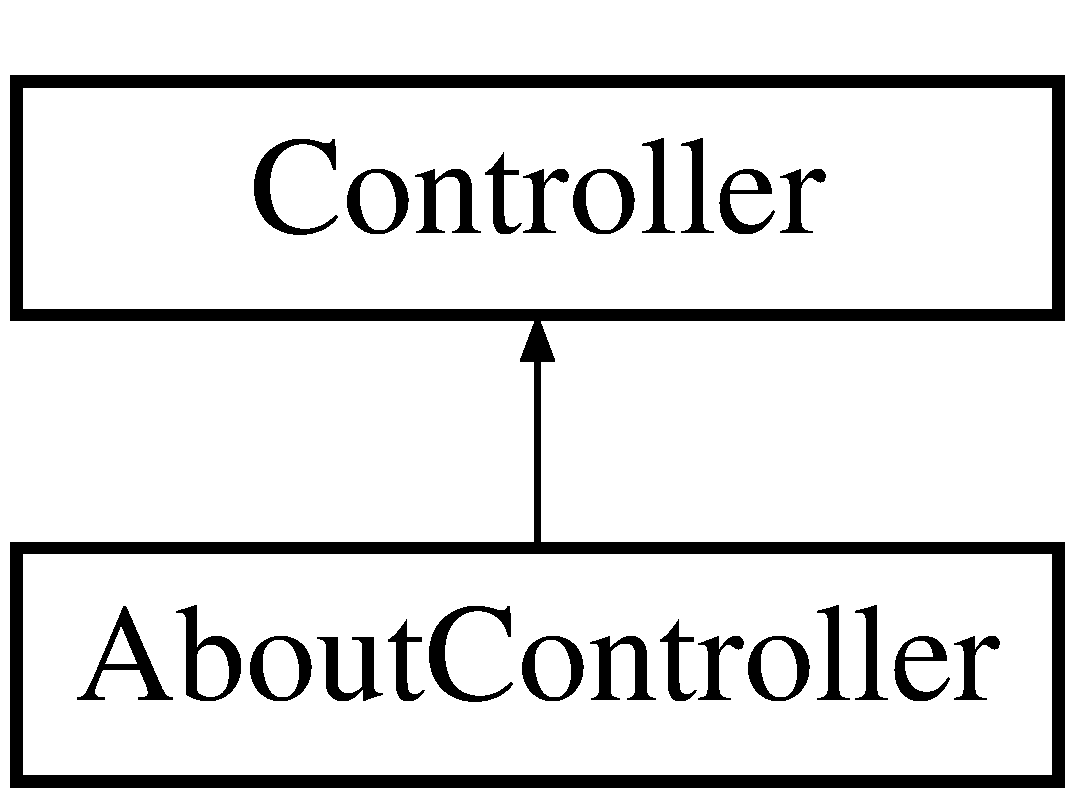
\includegraphics[height=2.000000cm]{class_about_controller}
\end{center}
\end{figure}
\subsection*{Public Member Functions}
\begin{DoxyCompactItemize}
\item 
{\bf index} (\$params=null)
\end{DoxyCompactItemize}
\subsection*{Additional Inherited Members}


\subsection{Member Function Documentation}
\index{About\-Controller@{About\-Controller}!index@{index}}
\index{index@{index}!AboutController@{About\-Controller}}
\subsubsection[{index}]{\setlength{\rightskip}{0pt plus 5cm}index (
\begin{DoxyParamCaption}
\item[{}]{\$params = {\ttfamily null}}
\end{DoxyParamCaption}
)}\label{class_about_controller_a749de566b023589025bfebbc37537d65}
Index de la page \char`\"{}à propos\char`\"{}

Met le titre de la page à 'À propos $|$ \doxyref{Diapazen}{p.}{namespace_diapazen}' Lance un render de la vue 'about'


\begin{DoxyParams}[1]{Parameters}
type & {\em \$params} & null par défaut \\
\hline
\end{DoxyParams}


The documentation for this class was generated from the following file\-:\begin{DoxyCompactItemize}
\item 
D\-:/\-Documents/\-Git\-Hub/diapazen/app/controller/About\-Controller.\-class.\-php\end{DoxyCompactItemize}

\section{Choice\-Model Class Reference}
\label{class_choice_model}\index{Choice\-Model@{Choice\-Model}}
Inheritance diagram for Choice\-Model\-:\begin{figure}[H]
\begin{center}
\leavevmode
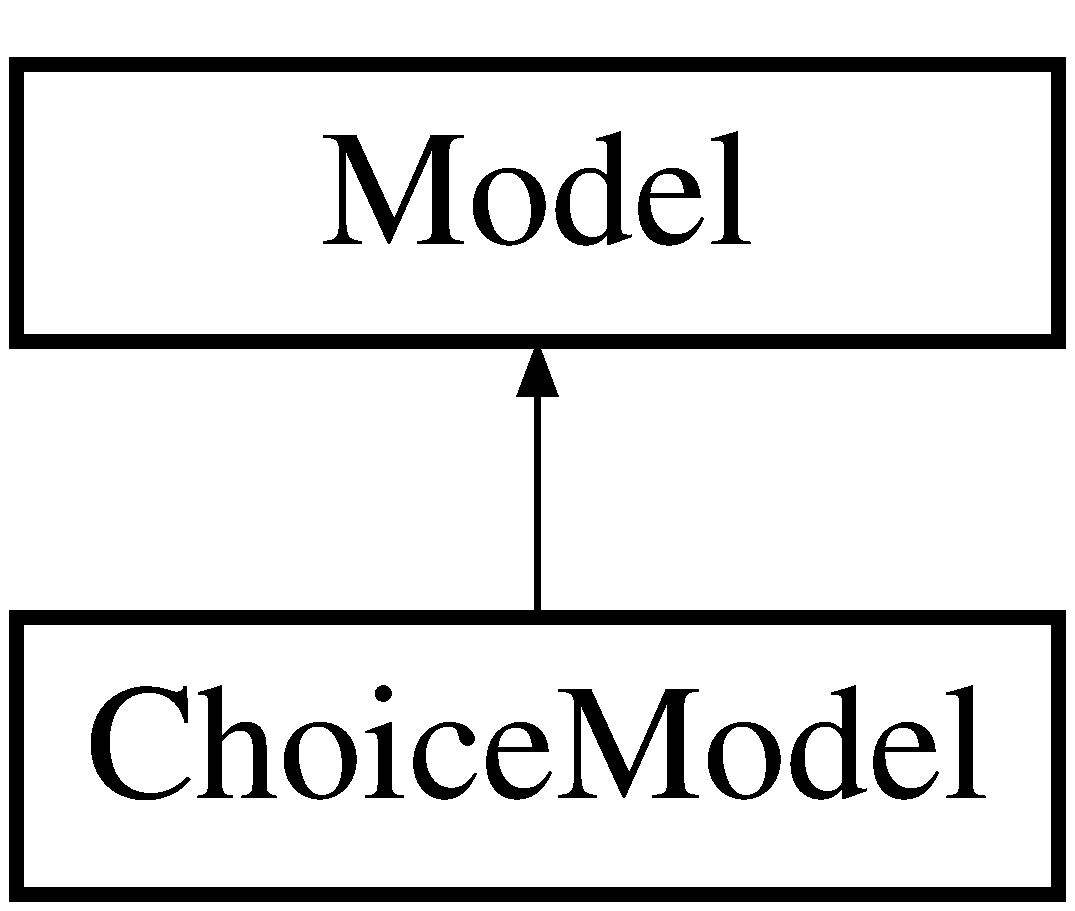
\includegraphics[height=2.000000cm]{class_choice_model}
\end{center}
\end{figure}
\subsection*{Public Member Functions}
\begin{DoxyCompactItemize}
\item 
{\bf \-\_\-\-\_\-construct} ()
\item 
{\bf add\-Choice} (\$title, \$poll\-Id)
\item 
{\bf update\-Choice} (\$title, \$id)
\item 
{\bf set\-Choice\-Title} (\$title)
\item 
{\bf get\-Choice\-Title} ()
\end{DoxyCompactItemize}
\subsection*{Additional Inherited Members}


\subsection{Constructor \& Destructor Documentation}
\index{Choice\-Model@{Choice\-Model}!\-\_\-\-\_\-construct@{\-\_\-\-\_\-construct}}
\index{\-\_\-\-\_\-construct@{\-\_\-\-\_\-construct}!ChoiceModel@{Choice\-Model}}
\subsubsection[{\-\_\-\-\_\-construct}]{\setlength{\rightskip}{0pt plus 5cm}\-\_\-\-\_\-construct (
\begin{DoxyParamCaption}
{}
\end{DoxyParamCaption}
)}\label{class_choice_model_a095c5d389db211932136b53f25f39685}
Constructeur par d�faut 

\subsection{Member Function Documentation}
\index{Choice\-Model@{Choice\-Model}!add\-Choice@{add\-Choice}}
\index{add\-Choice@{add\-Choice}!ChoiceModel@{Choice\-Model}}
\subsubsection[{add\-Choice}]{\setlength{\rightskip}{0pt plus 5cm}add\-Choice (
\begin{DoxyParamCaption}
\item[{}]{\$title, }
\item[{}]{\$poll\-Id}
\end{DoxyParamCaption}
)}\label{class_choice_model_a3014aa88191d070415381739c9bb7821}
Ajout d'un choix

Insert dans la base de donn�e 'dpz\-\_\-choices' un nouveau choix. M�thode utilis� gr�ce � la m�thode 'inser' de \doxyref{Model}{p.}{class_model}


\begin{DoxyParams}[1]{Parameters}
type & {\em \$title} & titre du choix \\
\hline
type & {\em \$poll\-Id} & id du sondage\\
\hline
\end{DoxyParams}
\begin{DoxyReturn}{Returns}
boolean true si l'ajout s'est bien ex�cut� sinon false 
\end{DoxyReturn}
\index{Choice\-Model@{Choice\-Model}!get\-Choice\-Title@{get\-Choice\-Title}}
\index{get\-Choice\-Title@{get\-Choice\-Title}!ChoiceModel@{Choice\-Model}}
\subsubsection[{get\-Choice\-Title}]{\setlength{\rightskip}{0pt plus 5cm}get\-Choice\-Title (
\begin{DoxyParamCaption}
{}
\end{DoxyParamCaption}
)}\label{class_choice_model_a7e8b7bec78fac1c4a2225604d5658ebd}
Getteur du titre du choix

\begin{DoxyReturn}{Returns}
type titre du choix 
\end{DoxyReturn}
\index{Choice\-Model@{Choice\-Model}!set\-Choice\-Title@{set\-Choice\-Title}}
\index{set\-Choice\-Title@{set\-Choice\-Title}!ChoiceModel@{Choice\-Model}}
\subsubsection[{set\-Choice\-Title}]{\setlength{\rightskip}{0pt plus 5cm}set\-Choice\-Title (
\begin{DoxyParamCaption}
\item[{}]{\$title}
\end{DoxyParamCaption}
)}\label{class_choice_model_a585b6c305e04e88c094aeab9d9e39888}
Setteur du titre du choix


\begin{DoxyParams}[1]{Parameters}
type & {\em \$title} & titre du choix \\
\hline
\end{DoxyParams}
\index{Choice\-Model@{Choice\-Model}!update\-Choice@{update\-Choice}}
\index{update\-Choice@{update\-Choice}!ChoiceModel@{Choice\-Model}}
\subsubsection[{update\-Choice}]{\setlength{\rightskip}{0pt plus 5cm}update\-Choice (
\begin{DoxyParamCaption}
\item[{}]{\$title, }
\item[{}]{\$id}
\end{DoxyParamCaption}
)}\label{class_choice_model_ad50c401b9a5705a5c307c9a17fd671a1}
Mise � Jour d'un choix

Met � jour dans la base de donn�e 'dpz\-\_\-choices' du titre et de l'id du choix. M�thode utilis� gr�ce � la m�thode 'update\-Where' de \doxyref{Model}{p.}{class_model}


\begin{DoxyParams}[1]{Parameters}
type & {\em \$title} & titre du choix \\
\hline
type & {\em \$id} & id du choix \\
\hline
\end{DoxyParams}
\begin{DoxyReturn}{Returns}
boolean true si l'ajout s'est bien ex�cut� sinon false 
\end{DoxyReturn}


The documentation for this class was generated from the following file\-:\begin{DoxyCompactItemize}
\item 
D\-:/\-Documents/\-Git\-Hub/diapazen/app/model/Choice\-Model.\-class.\-php\end{DoxyCompactItemize}

\section{Config Class Reference}
\label{class_config}\index{Config@{Config}}
\subsection*{Static Public Member Functions}
\begin{DoxyCompactItemize}
\item 
static {\bf get\-Database\-Config} (\$config\-Name= '')
\end{DoxyCompactItemize}


\subsection{Member Function Documentation}
\index{Config@{Config}!get\-Database\-Config@{get\-Database\-Config}}
\index{get\-Database\-Config@{get\-Database\-Config}!Config@{Config}}
\subsubsection[{get\-Database\-Config}]{\setlength{\rightskip}{0pt plus 5cm}static get\-Database\-Config (
\begin{DoxyParamCaption}
\item[{}]{\$config\-Name = {\ttfamily ''}}
\end{DoxyParamCaption}
)\hspace{0.3cm}{\ttfamily [static]}}\label{class_config_a42533076e390d1cf7d4b1d2e2ea3413d}
Récupère la configuration de la base de donnée voulue.


\begin{DoxyParams}[1]{Parameters}
string & {\em \$config\-Name} & Nom de la configuration à utiliser \\
\hline
\end{DoxyParams}
\begin{DoxyReturn}{Returns}
array La configuration voulue 
\end{DoxyReturn}


The documentation for this class was generated from the following file\-:\begin{DoxyCompactItemize}
\item 
D\-:/\-Documents/\-Git\-Hub/diapazen/config/Config.\-class.\-php\end{DoxyCompactItemize}

\section{Controller Class Reference}
\label{class_controller}\index{Controller@{Controller}}
Inheritance diagram for Controller\-:\begin{figure}[H]
\begin{center}
\leavevmode
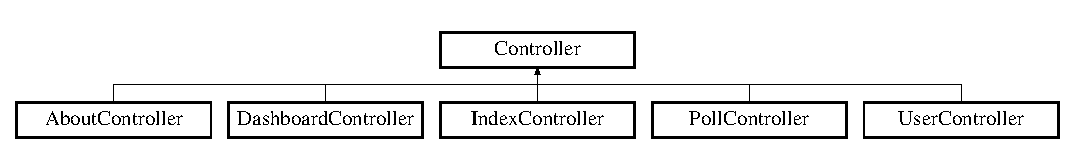
\includegraphics[height=1.623188cm]{class_controller}
\end{center}
\end{figure}
\subsection*{Public Member Functions}
\begin{DoxyCompactItemize}
\item 
{\bf \-\_\-\-\_\-construct} (\$request)
\item 
{\bf render} (\$view)
\item 
{\bf e404} ()
\item 
{\bf get\-Path} (\$filename)
\item 
{\bf get\-Header} ()
\item 
{\bf get\-Footer} ()
\item 
{\bf get\-Ariadne\-Thread} ()
\item 
{\bf get\-Home\-Url} ()
\item 
{\bf set\-User\-Connected} (\$user\-Infos)
\item 
{\bf set\-User\-Disconnected} ()
\item 
{\bf is\-User\-Connected} ()
\item 
{\bf get\-User\-Info} (\$key)
\item 
{\bf set\-User\-Info} (\$key, \$value)
\end{DoxyCompactItemize}
\subsection*{Protected Member Functions}
\begin{DoxyCompactItemize}
\item 
{\bf load\-Model} (\$model)
\item 
{\bf get\-Model} ()
\item 
{\bf set} (\$key, \$value)
\end{DoxyCompactItemize}
\subsection*{Protected Attributes}
\begin{DoxyCompactItemize}
\item 
{\bfseries \$m\-Model}\label{class_controller_a192d6493adb043f7a7f016b6070e1257}

\item 
{\bfseries \$m\-Request}\label{class_controller_a6f829f0dd59d9c64b6023f1fc9062c4a}

\item 
{\bfseries \$m\-Vars} = array()\label{class_controller_a58a15773596277a8f58eb4d1d500ed02}

\end{DoxyCompactItemize}


\subsection{Constructor \& Destructor Documentation}
\index{Controller@{Controller}!\-\_\-\-\_\-construct@{\-\_\-\-\_\-construct}}
\index{\-\_\-\-\_\-construct@{\-\_\-\-\_\-construct}!Controller@{Controller}}
\subsubsection[{\-\_\-\-\_\-construct}]{\setlength{\rightskip}{0pt plus 5cm}\-\_\-\-\_\-construct (
\begin{DoxyParamCaption}
\item[{}]{\$request}
\end{DoxyParamCaption}
)}\label{class_controller_a81bdf9b2f742c664208230ca9ad44f28}
Constructeur 
\begin{DoxyParams}{Parameters}
{\em \doxyref{Request}{p.}{class_request}} & request Requête H\-T\-T\-P \\
\hline
\end{DoxyParams}


\subsection{Member Function Documentation}
\index{Controller@{Controller}!e404@{e404}}
\index{e404@{e404}!Controller@{Controller}}
\subsubsection[{e404}]{\setlength{\rightskip}{0pt plus 5cm}e404 (
\begin{DoxyParamCaption}
{}
\end{DoxyParamCaption}
)}\label{class_controller_a2163fbc31872b3c99dbfafe45a768fbb}
Affiche l'erreur 404 \index{Controller@{Controller}!get\-Ariadne\-Thread@{get\-Ariadne\-Thread}}
\index{get\-Ariadne\-Thread@{get\-Ariadne\-Thread}!Controller@{Controller}}
\subsubsection[{get\-Ariadne\-Thread}]{\setlength{\rightskip}{0pt plus 5cm}get\-Ariadne\-Thread (
\begin{DoxyParamCaption}
{}
\end{DoxyParamCaption}
)}\label{class_controller_a71e04a4cb75e764599a305b1089945bd}
Inclut le fichier du fil d'arianne. A utiliser dans les fichiers de vue

\begin{DoxyReturn}{Returns}
void Rien 
\end{DoxyReturn}
\index{Controller@{Controller}!get\-Footer@{get\-Footer}}
\index{get\-Footer@{get\-Footer}!Controller@{Controller}}
\subsubsection[{get\-Footer}]{\setlength{\rightskip}{0pt plus 5cm}get\-Footer (
\begin{DoxyParamCaption}
{}
\end{DoxyParamCaption}
)}\label{class_controller_afd65368c3ca63e81eeefe796a85201ba}
Inclut le fichier de pied de page. A utiliser dans les fichiers de vue

\begin{DoxyReturn}{Returns}
void Rien 
\end{DoxyReturn}
\index{Controller@{Controller}!get\-Header@{get\-Header}}
\index{get\-Header@{get\-Header}!Controller@{Controller}}
\subsubsection[{get\-Header}]{\setlength{\rightskip}{0pt plus 5cm}get\-Header (
\begin{DoxyParamCaption}
{}
\end{DoxyParamCaption}
)}\label{class_controller_a614834f1605e407376028e8c82298c82}
Inclut le fichier d'entête. A utiliser dans les fichiers de vue

\begin{DoxyReturn}{Returns}
void Rien 
\end{DoxyReturn}
\index{Controller@{Controller}!get\-Home\-Url@{get\-Home\-Url}}
\index{get\-Home\-Url@{get\-Home\-Url}!Controller@{Controller}}
\subsubsection[{get\-Home\-Url}]{\setlength{\rightskip}{0pt plus 5cm}get\-Home\-Url (
\begin{DoxyParamCaption}
{}
\end{DoxyParamCaption}
)}\label{class_controller_ada8fa4fecbe408317fc25c98ab506296}
Récupère l'url de la page d'accueil

\begin{DoxyReturn}{Returns}
void Rien 
\end{DoxyReturn}
\index{Controller@{Controller}!get\-Model@{get\-Model}}
\index{get\-Model@{get\-Model}!Controller@{Controller}}
\subsubsection[{get\-Model}]{\setlength{\rightskip}{0pt plus 5cm}get\-Model (
\begin{DoxyParamCaption}
{}
\end{DoxyParamCaption}
)\hspace{0.3cm}{\ttfamily [protected]}}\label{class_controller_a0a086ca877b41192556a2de7e4a97b98}
Retourne le modèle de données \begin{DoxyReturn}{Returns}
\doxyref{Model}{p.}{class_model} model Modèle de données 
\end{DoxyReturn}
\index{Controller@{Controller}!get\-Path@{get\-Path}}
\index{get\-Path@{get\-Path}!Controller@{Controller}}
\subsubsection[{get\-Path}]{\setlength{\rightskip}{0pt plus 5cm}get\-Path (
\begin{DoxyParamCaption}
\item[{}]{\$filename}
\end{DoxyParamCaption}
)}\label{class_controller_af7b2ad7d99459b3e105ca7ba0fa14069}
Récupère le chemin d'un fichier css,js,png ...

Exemple d'utilisation\-: \$this-\/$>$get\-Path('css/style.\-css'); Donne le chemin du fichier style.\-css


\begin{DoxyParams}{Parameters}
{\em string} & filename chemin relatif du fichier \\
\hline
\end{DoxyParams}
\begin{DoxyReturn}{Returns}
string chemin complet du fichier 
\end{DoxyReturn}
\index{Controller@{Controller}!get\-User\-Info@{get\-User\-Info}}
\index{get\-User\-Info@{get\-User\-Info}!Controller@{Controller}}
\subsubsection[{get\-User\-Info}]{\setlength{\rightskip}{0pt plus 5cm}get\-User\-Info (
\begin{DoxyParamCaption}
\item[{}]{\$key}
\end{DoxyParamCaption}
)}\label{class_controller_a918b69dab8f9fe8e0cc8a7f5d530d1e4}
Récupère les informations de l'utilisateur (stocké en session)


\begin{DoxyParams}{Parameters}
{\em string} & key clé \\
\hline
\end{DoxyParams}
\begin{DoxyReturn}{Returns}
string Information voulue 
\end{DoxyReturn}
\index{Controller@{Controller}!is\-User\-Connected@{is\-User\-Connected}}
\index{is\-User\-Connected@{is\-User\-Connected}!Controller@{Controller}}
\subsubsection[{is\-User\-Connected}]{\setlength{\rightskip}{0pt plus 5cm}is\-User\-Connected (
\begin{DoxyParamCaption}
{}
\end{DoxyParamCaption}
)}\label{class_controller_aba0fa3d6e5fdb720397f057b6f98aca9}
L'utilisateur est-\/il connecté ?

\begin{DoxyReturn}{Returns}
bool Vrai si il est connecté, Faux sinon 
\end{DoxyReturn}
\index{Controller@{Controller}!load\-Model@{load\-Model}}
\index{load\-Model@{load\-Model}!Controller@{Controller}}
\subsubsection[{load\-Model}]{\setlength{\rightskip}{0pt plus 5cm}load\-Model (
\begin{DoxyParamCaption}
\item[{}]{\$model}
\end{DoxyParamCaption}
)\hspace{0.3cm}{\ttfamily [protected]}}\label{class_controller_ab25941a477cf4f0f98439627cefbca08}
Charge le modèle de données 
\begin{DoxyParams}{Parameters}
{\em \doxyref{Model}{p.}{class_model}} & model Modèle de données \\
\hline
\end{DoxyParams}
\index{Controller@{Controller}!render@{render}}
\index{render@{render}!Controller@{Controller}}
\subsubsection[{render}]{\setlength{\rightskip}{0pt plus 5cm}render (
\begin{DoxyParamCaption}
\item[{}]{\$view}
\end{DoxyParamCaption}
)}\label{class_controller_a402c6c924d6f21d17da89bc29e65956d}
Fait le rendu de la vue


\begin{DoxyParams}{Parameters}
{\em string} & filename chemin relatif du fichier \\
\hline
\end{DoxyParams}
\begin{DoxyReturn}{Returns}
void Rien 
\end{DoxyReturn}
\index{Controller@{Controller}!set@{set}}
\index{set@{set}!Controller@{Controller}}
\subsubsection[{set}]{\setlength{\rightskip}{0pt plus 5cm}set (
\begin{DoxyParamCaption}
\item[{}]{\$key, }
\item[{}]{\$value}
\end{DoxyParamCaption}
)\hspace{0.3cm}{\ttfamily [protected]}}\label{class_controller_aab787bd83f84f4215dceb35f7c305eee}
Ajoute une variable pour la vue


\begin{DoxyParams}{Parameters}
{\em string} & filename chemin relatif du fichier \\
\hline
\end{DoxyParams}
\begin{DoxyReturn}{Returns}
void Rien 
\end{DoxyReturn}
\index{Controller@{Controller}!set\-User\-Connected@{set\-User\-Connected}}
\index{set\-User\-Connected@{set\-User\-Connected}!Controller@{Controller}}
\subsubsection[{set\-User\-Connected}]{\setlength{\rightskip}{0pt plus 5cm}set\-User\-Connected (
\begin{DoxyParamCaption}
\item[{}]{\$user\-Infos}
\end{DoxyParamCaption}
)}\label{class_controller_ad81438963e946370065e5018c4d0fe49}
Connecte l'utilisateur

\begin{DoxyReturn}{Returns}
void Rien 
\end{DoxyReturn}
\index{Controller@{Controller}!set\-User\-Disconnected@{set\-User\-Disconnected}}
\index{set\-User\-Disconnected@{set\-User\-Disconnected}!Controller@{Controller}}
\subsubsection[{set\-User\-Disconnected}]{\setlength{\rightskip}{0pt plus 5cm}set\-User\-Disconnected (
\begin{DoxyParamCaption}
{}
\end{DoxyParamCaption}
)}\label{class_controller_a4709000ecaa3d4cc3d6ad2a0954d75f3}
Déconnecte l'utilisateur

\begin{DoxyReturn}{Returns}
void Rien 
\end{DoxyReturn}
\index{Controller@{Controller}!set\-User\-Info@{set\-User\-Info}}
\index{set\-User\-Info@{set\-User\-Info}!Controller@{Controller}}
\subsubsection[{set\-User\-Info}]{\setlength{\rightskip}{0pt plus 5cm}set\-User\-Info (
\begin{DoxyParamCaption}
\item[{}]{\$key, }
\item[{}]{\$value}
\end{DoxyParamCaption}
)}\label{class_controller_a3b5b4a9a7d7b387fef4c37770c604c44}
Définit les informations de l'utilisateur (stocké en session)


\begin{DoxyParams}{Parameters}
{\em string} & key clé \\
\hline
{\em string} & Information voulue \\
\hline
\end{DoxyParams}


The documentation for this class was generated from the following file\-:\begin{DoxyCompactItemize}
\item 
D\-:/\-Documents/\-Git\-Hub/diapazen/system/Controller.\-class.\-php\end{DoxyCompactItemize}

\section{Core\-Exception Class Reference}
\label{class_core_exception}\index{Core\-Exception@{Core\-Exception}}
Inheritance diagram for Core\-Exception\-:\begin{figure}[H]
\begin{center}
\leavevmode
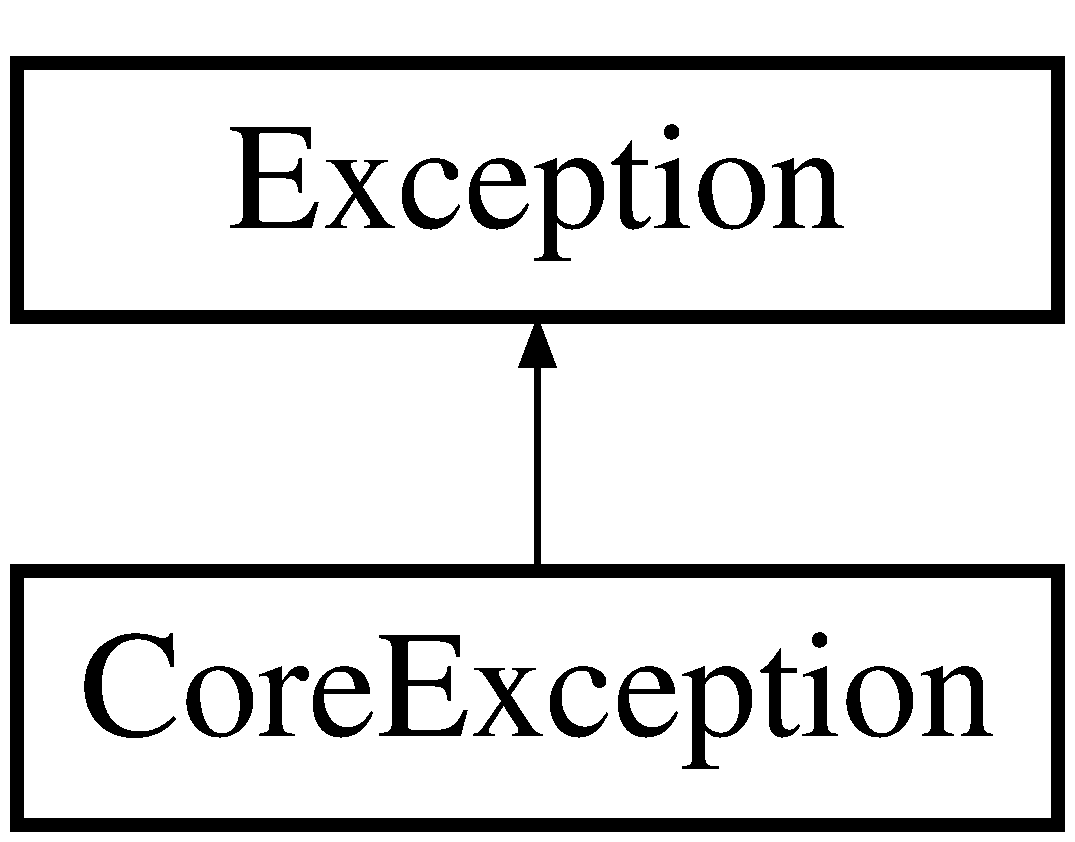
\includegraphics[height=2.000000cm]{class_core_exception}
\end{center}
\end{figure}
\subsection*{Public Member Functions}
\begin{DoxyCompactItemize}
\item 
{\bf \-\_\-\-\_\-construct} (\$e\-Message, \$e\-Code=0, \$log=false)
\item 
{\bf get\-Message\-Formate} ()
\end{DoxyCompactItemize}
\subsection*{Protected Attributes}
\begin{DoxyCompactItemize}
\item 
{\bfseries \$me\-Message}\label{class_core_exception_a06f7f5eb58544af93bc37a46f5790576}

\item 
{\bfseries \$me\-Code}\label{class_core_exception_a57d7256df9f104dda7403543b14d8290}

\item 
{\bfseries \$me\-File}\label{class_core_exception_a1dcbc5f489cc47c6608761e37746ac32}

\item 
{\bfseries \$me\-Line}\label{class_core_exception_a363869009d1f0ee3eb4bedb5ba3593d3}

\item 
{\bfseries \$me\-Date}\label{class_core_exception_a8202f62ce9b8485cf8bcdcc34637ef5d}

\end{DoxyCompactItemize}


\subsection{Constructor \& Destructor Documentation}
\index{Core\-Exception@{Core\-Exception}!\-\_\-\-\_\-construct@{\-\_\-\-\_\-construct}}
\index{\-\_\-\-\_\-construct@{\-\_\-\-\_\-construct}!CoreException@{Core\-Exception}}
\subsubsection[{\-\_\-\-\_\-construct}]{\setlength{\rightskip}{0pt plus 5cm}\-\_\-\-\_\-construct (
\begin{DoxyParamCaption}
\item[{}]{\$e\-Message, }
\item[{}]{\$e\-Code = {\ttfamily 0}, }
\item[{}]{\$log = {\ttfamily false}}
\end{DoxyParamCaption}
)}\label{class_core_exception_a0b919d549249df87cf133c4be12b6560}
Constructeur de la classe d exception

Constructeur de la classe d exception personnalisé, qui cree notre exception mais aussi utilise un systeme de log


\begin{DoxyParams}{Parameters}
{\em string} & e\-Message message de l exception \\
\hline
{\em unsigned} & int e\-Code code de l exception \\
\hline
\end{DoxyParams}


\subsection{Member Function Documentation}
\index{Core\-Exception@{Core\-Exception}!get\-Message\-Formate@{get\-Message\-Formate}}
\index{get\-Message\-Formate@{get\-Message\-Formate}!CoreException@{Core\-Exception}}
\subsubsection[{get\-Message\-Formate}]{\setlength{\rightskip}{0pt plus 5cm}get\-Message\-Formate (
\begin{DoxyParamCaption}
{}
\end{DoxyParamCaption}
)}\label{class_core_exception_a82a587d57e8d4a4d1eac58914b6cb5d1}
Formate le message

\begin{DoxyReturn}{Returns}
string message\-Formate message de l exception formaté 
\end{DoxyReturn}


The documentation for this class was generated from the following file\-:\begin{DoxyCompactItemize}
\item 
D\-:/\-Documents/\-Git\-Hub/diapazen/system/Core\-Exception.\-class.\-php\end{DoxyCompactItemize}

\section{Core\-Loader Class Reference}
\label{class_core_loader}\index{Core\-Loader@{Core\-Loader}}
\subsection*{Static Public Member Functions}
\begin{DoxyCompactItemize}
\item 
static {\bf get\-Instance} ()
\end{DoxyCompactItemize}


\subsection{Member Function Documentation}
\index{Core\-Loader@{Core\-Loader}!get\-Instance@{get\-Instance}}
\index{get\-Instance@{get\-Instance}!CoreLoader@{Core\-Loader}}
\subsubsection[{get\-Instance}]{\setlength{\rightskip}{0pt plus 5cm}static get\-Instance (
\begin{DoxyParamCaption}
{}
\end{DoxyParamCaption}
)\hspace{0.3cm}{\ttfamily [static]}}\label{class_core_loader_ac93fbec81f07e5d15f80db907e63dc10}
Récuperation d'un loader

Permet de récuperer un loader selon le design pattern singleton. 

The documentation for this class was generated from the following file\-:\begin{DoxyCompactItemize}
\item 
D\-:/\-Documents/\-Git\-Hub/diapazen/system/Core\-Loader.\-class.\-php\end{DoxyCompactItemize}

\section{Core\-Logger Class Reference}
\label{class_core_logger}\index{Core\-Logger@{Core\-Logger}}
\subsection*{Public Member Functions}
\begin{DoxyCompactItemize}
\item 
{\bf set\-Writer} (\$Obj\-Writer)
\item 
{\bf log} (\$message, \$level)
\end{DoxyCompactItemize}
\subsection*{Static Public Member Functions}
\begin{DoxyCompactItemize}
\item 
static {\bf get\-Instance} ()
\end{DoxyCompactItemize}


\subsection{Member Function Documentation}
\index{Core\-Logger@{Core\-Logger}!get\-Instance@{get\-Instance}}
\index{get\-Instance@{get\-Instance}!CoreLogger@{Core\-Logger}}
\subsubsection[{get\-Instance}]{\setlength{\rightskip}{0pt plus 5cm}static get\-Instance (
\begin{DoxyParamCaption}
{}
\end{DoxyParamCaption}
)\hspace{0.3cm}{\ttfamily [static]}}\label{class_core_logger_ac93fbec81f07e5d15f80db907e63dc10}
Récuperation d'un logger

Permet de récuperer un logger selon le design pattern singleton. \index{Core\-Logger@{Core\-Logger}!log@{log}}
\index{log@{log}!CoreLogger@{Core\-Logger}}
\subsubsection[{log}]{\setlength{\rightskip}{0pt plus 5cm}log (
\begin{DoxyParamCaption}
\item[{}]{\$message, }
\item[{}]{\$level}
\end{DoxyParamCaption}
)}\label{class_core_logger_a9eb5aa8b14114f554518dfb38450824b}
Log

Long description


\begin{DoxyParams}{Parameters}
{\em String} & message message du log \\
\hline
{\em String} & level niveau du log \\
\hline
\end{DoxyParams}
\index{Core\-Logger@{Core\-Logger}!set\-Writer@{set\-Writer}}
\index{set\-Writer@{set\-Writer}!CoreLogger@{Core\-Logger}}
\subsubsection[{set\-Writer}]{\setlength{\rightskip}{0pt plus 5cm}set\-Writer (
\begin{DoxyParamCaption}
\item[{}]{\$\-Obj\-Writer}
\end{DoxyParamCaption}
)}\label{class_core_logger_a4b6b6ce4ba59214101ce027699e155ac}
Affecte un writer

Determine quel objet writter est utiliser pour ecrire notre log


\begin{DoxyParams}{Parameters}
{\em type} & Obj\-Writer\\
\hline
\end{DoxyParams}
\begin{DoxyReturn}{Returns}
boolean affectation reussi 
\end{DoxyReturn}


The documentation for this class was generated from the following file\-:\begin{DoxyCompactItemize}
\item 
D\-:/\-Documents/\-Git\-Hub/diapazen/system/Core\-Logger.\-class.\-php\end{DoxyCompactItemize}

\section{core\-Singleton Class Reference}
\label{classcore_singleton}\index{core\-Singleton@{core\-Singleton}}
\subsection*{Static Public Member Functions}
\begin{DoxyCompactItemize}
\item 
static {\bfseries \-\_\-\-\_\-call\-Static} (\$name, array \$arguments=array())\label{classcore_singleton_a7b34b1bb7f5045d7d05e6b5bd907aabb}

\end{DoxyCompactItemize}
\subsection*{Static Public Attributes}
\begin{DoxyCompactItemize}
\item 
static {\bfseries \$namespace} = \-\_\-\-\_\-\-N\-A\-M\-E\-S\-P\-A\-C\-E\-\_\-\-\_\-\label{classcore_singleton_a3825c9b9060c2d6ef594385997cd60aa}

\end{DoxyCompactItemize}
\subsection*{Static Protected Attributes}
\begin{DoxyCompactItemize}
\item 
static {\bfseries \$\-\_\-instances}\label{classcore_singleton_a184e634b52323f577a8d345206d690a1}

\end{DoxyCompactItemize}


The documentation for this class was generated from the following file\-:\begin{DoxyCompactItemize}
\item 
D\-:/\-Documents/\-Git\-Hub/diapazen/system/Singleton.\-class.\-php.\-php\end{DoxyCompactItemize}

\section{Dashboard\-Controller Class Reference}
\label{class_dashboard_controller}\index{Dashboard\-Controller@{Dashboard\-Controller}}
Inheritance diagram for Dashboard\-Controller\-:\begin{figure}[H]
\begin{center}
\leavevmode
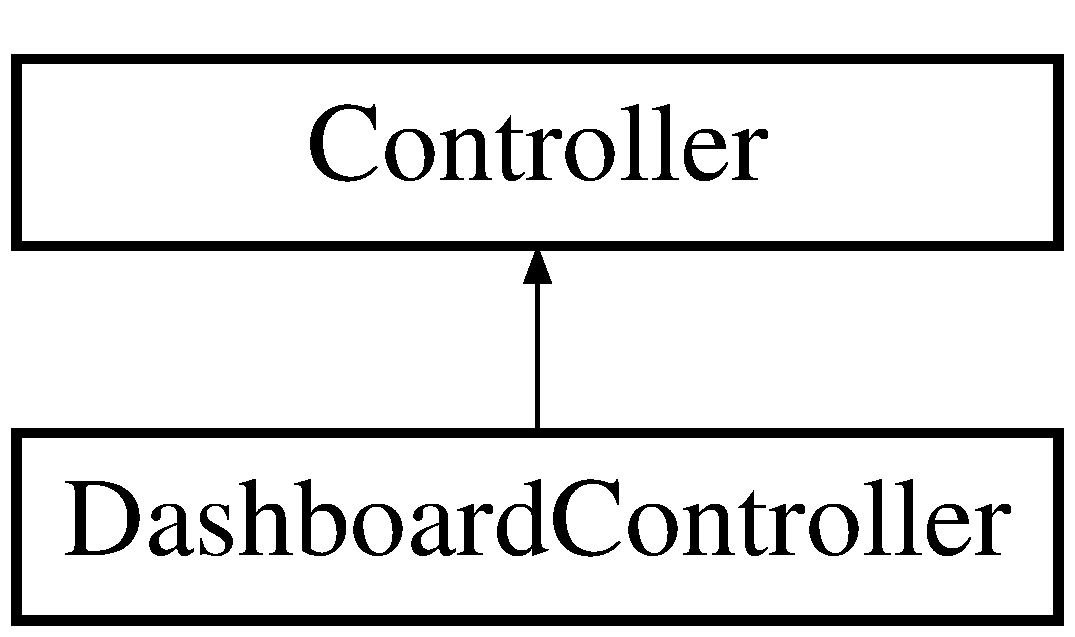
\includegraphics[height=2.000000cm]{class_dashboard_controller}
\end{center}
\end{figure}
\subsection*{Public Member Functions}
\begin{DoxyCompactItemize}
\item 
{\bf index} (\$params=null)
\end{DoxyCompactItemize}
\subsection*{Additional Inherited Members}


\subsection{Member Function Documentation}
\index{Dashboard\-Controller@{Dashboard\-Controller}!index@{index}}
\index{index@{index}!DashboardController@{Dashboard\-Controller}}
\subsubsection[{index}]{\setlength{\rightskip}{0pt plus 5cm}index (
\begin{DoxyParamCaption}
\item[{}]{\$params = {\ttfamily null}}
\end{DoxyParamCaption}
)}\label{class_dashboard_controller_a749de566b023589025bfebbc37537d65}
Index du Dashboard

Récupère le model 'poll' Gère \-:
\begin{DoxyItemize}
\item Met le titre de la page à 'Tableau de bord $|$ \doxyref{Diapazen}{p.}{namespace_diapazen}'.
\item La fermeture de sondage
\item Met à jour les sondages expirés dans la B\-D\-D
\item Lance le render de la vue 'dashboard' (si l'utilisateur est connecté)
\item Retourne à la page d'accueil (si l'utilisateur n'est aps connecté)
\end{DoxyItemize}


\begin{DoxyParams}[1]{Parameters}
type & {\em \$params} & null par défaut \\
\hline
\end{DoxyParams}


The documentation for this class was generated from the following file\-:\begin{DoxyCompactItemize}
\item 
D\-:/\-Documents/\-Git\-Hub/diapazen/app/controller/Dashboard\-Controller.\-class.\-php\end{DoxyCompactItemize}

\section{Downloader\-File\-Util Class Reference}
\label{class_downloader_file_util}\index{Downloader\-File\-Util@{Downloader\-File\-Util}}
\subsection*{Public Member Functions}
\begin{DoxyCompactItemize}
\item 
{\bf \-\_\-\-\_\-construct} (\$filename, \$filepath= '', \$newfilename= '')
\item 
{\bf force\-Download} ()
\end{DoxyCompactItemize}
\subsection*{Static Public Member Functions}
\begin{DoxyCompactItemize}
\item 
static {\bf clean\-Path} (\$path)
\item 
static {\bf get\-Extension} (\$file)
\end{DoxyCompactItemize}


\subsection{Constructor \& Destructor Documentation}
\index{Downloader\-File\-Util@{Downloader\-File\-Util}!\-\_\-\-\_\-construct@{\-\_\-\-\_\-construct}}
\index{\-\_\-\-\_\-construct@{\-\_\-\-\_\-construct}!DownloaderFileUtil@{Downloader\-File\-Util}}
\subsubsection[{\-\_\-\-\_\-construct}]{\setlength{\rightskip}{0pt plus 5cm}\-\_\-\-\_\-construct (
\begin{DoxyParamCaption}
\item[{}]{\$filename, }
\item[{}]{\$filepath = {\ttfamily ''}, }
\item[{}]{\$newfilename = {\ttfamily ''}}
\end{DoxyParamCaption}
)}\label{class_downloader_file_util_a64fddf6c6ab12a72fe6287b63105d297}
Constructeur du downloader

Permet de choisir les informations utile pour le telechargement


\begin{DoxyParams}{Parameters}
{\em Sting} & filename nom du fichier a télécharger \\
\hline
{\em Sting} & filepath lien vers le fichier \\
\hline
{\em Sting} & newfilename nom du fichier pour l'utilisateur \\
\hline
\end{DoxyParams}


\subsection{Member Function Documentation}
\index{Downloader\-File\-Util@{Downloader\-File\-Util}!clean\-Path@{clean\-Path}}
\index{clean\-Path@{clean\-Path}!DownloaderFileUtil@{Downloader\-File\-Util}}
\subsubsection[{clean\-Path}]{\setlength{\rightskip}{0pt plus 5cm}static clean\-Path (
\begin{DoxyParamCaption}
\item[{}]{\$path}
\end{DoxyParamCaption}
)\hspace{0.3cm}{\ttfamily [static]}}\label{class_downloader_file_util_ab97c806c355ce59b5a2c425444ddfa0b}
clean\-Path

Rend le chemin vers le fichier correct


\begin{DoxyParams}{Parameters}
{\em string} & path chemin \\
\hline
\end{DoxyParams}
\begin{DoxyReturn}{Returns}
string path chemin 
\end{DoxyReturn}
\index{Downloader\-File\-Util@{Downloader\-File\-Util}!force\-Download@{force\-Download}}
\index{force\-Download@{force\-Download}!DownloaderFileUtil@{Downloader\-File\-Util}}
\subsubsection[{force\-Download}]{\setlength{\rightskip}{0pt plus 5cm}force\-Download (
\begin{DoxyParamCaption}
{}
\end{DoxyParamCaption}
)}\label{class_downloader_file_util_a31cf5274dbb0c7b89d01a13a17c38bae}
Lance le telechargement

Il est forcé, cad qu'un fichier pdf ne s'ouvrira pas mais devra etre telecharge

\begin{DoxyReturn}{Returns}
boolean resultat du telechargement 
\end{DoxyReturn}
\index{Downloader\-File\-Util@{Downloader\-File\-Util}!get\-Extension@{get\-Extension}}
\index{get\-Extension@{get\-Extension}!DownloaderFileUtil@{Downloader\-File\-Util}}
\subsubsection[{get\-Extension}]{\setlength{\rightskip}{0pt plus 5cm}static get\-Extension (
\begin{DoxyParamCaption}
\item[{}]{\$file}
\end{DoxyParamCaption}
)\hspace{0.3cm}{\ttfamily [static]}}\label{class_downloader_file_util_af86d98bc73b99d35a82728f16fd19151}
Renvoie l'extension du fichier

Long description


\begin{DoxyParams}{Parameters}
{\em String} & nom fichier \\
\hline
\end{DoxyParams}
\begin{DoxyReturn}{Returns}
string extension 
\end{DoxyReturn}


The documentation for this class was generated from the following file\-:\begin{DoxyCompactItemize}
\item 
D\-:/\-Documents/\-Git\-Hub/diapazen/util/Downloader\-File\-Util.\-class.\-php\end{DoxyCompactItemize}

\section{Index\-Controller Class Reference}
\label{class_index_controller}\index{Index\-Controller@{Index\-Controller}}
Inheritance diagram for Index\-Controller\-:\begin{figure}[H]
\begin{center}
\leavevmode
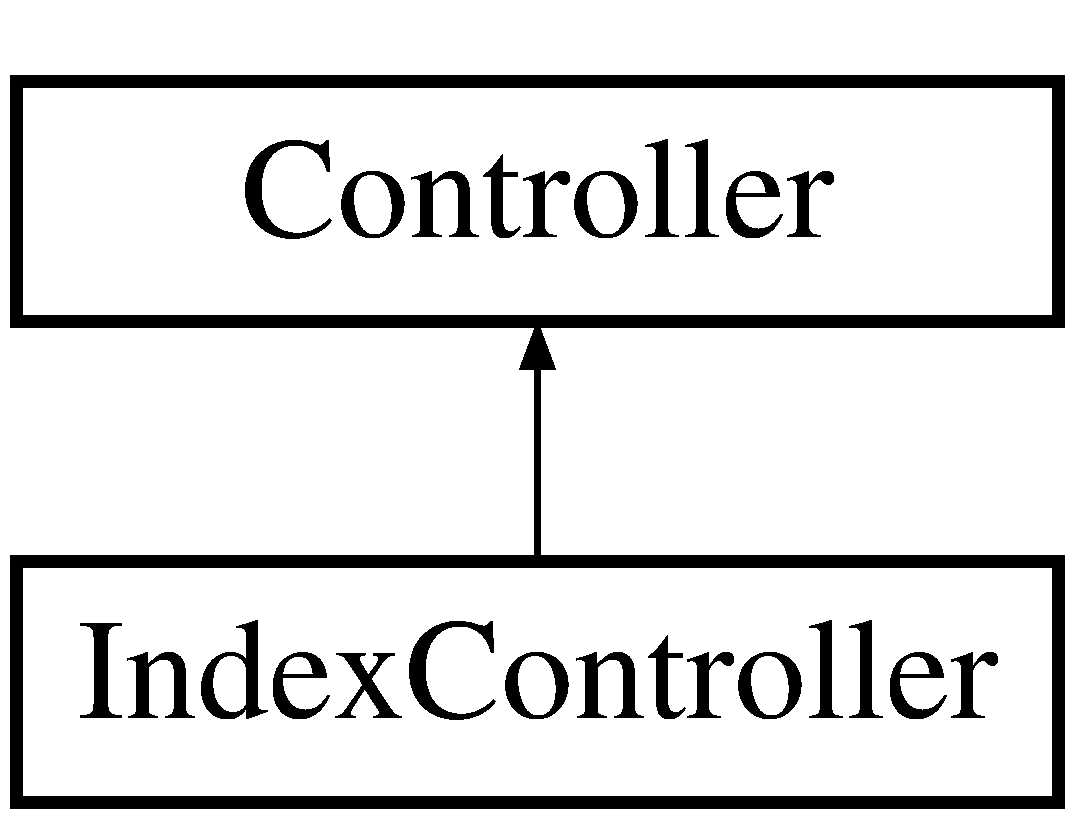
\includegraphics[height=2.000000cm]{class_index_controller}
\end{center}
\end{figure}
\subsection*{Public Member Functions}
\begin{DoxyCompactItemize}
\item 
{\bf index} (\$params=null)
\end{DoxyCompactItemize}
\subsection*{Additional Inherited Members}


\subsection{Member Function Documentation}
\index{Index\-Controller@{Index\-Controller}!index@{index}}
\index{index@{index}!IndexController@{Index\-Controller}}
\subsubsection[{index}]{\setlength{\rightskip}{0pt plus 5cm}index (
\begin{DoxyParamCaption}
\item[{}]{\$params = {\ttfamily null}}
\end{DoxyParamCaption}
)}\label{class_index_controller_a749de566b023589025bfebbc37537d65}
On set la variable à afficher sur dans la vue et on teste si l'utilisateur est conn�cter. Si tel est le cas alors on redirige vers le dashboard, sino on se rend sur la page home. 
\begin{DoxyParams}[1]{Parameters}
type & {\em \$params} & \\
\hline
\end{DoxyParams}


The documentation for this class was generated from the following file\-:\begin{DoxyCompactItemize}
\item 
D\-:/\-Documents/\-Git\-Hub/diapazen/app/controller/Index\-Controller.\-class.\-php\end{DoxyCompactItemize}

\section{I\-Writer Interface Reference}
\label{interface_i_writer}\index{I\-Writer@{I\-Writer}}
Inheritance diagram for I\-Writer\-:\begin{figure}[H]
\begin{center}
\leavevmode
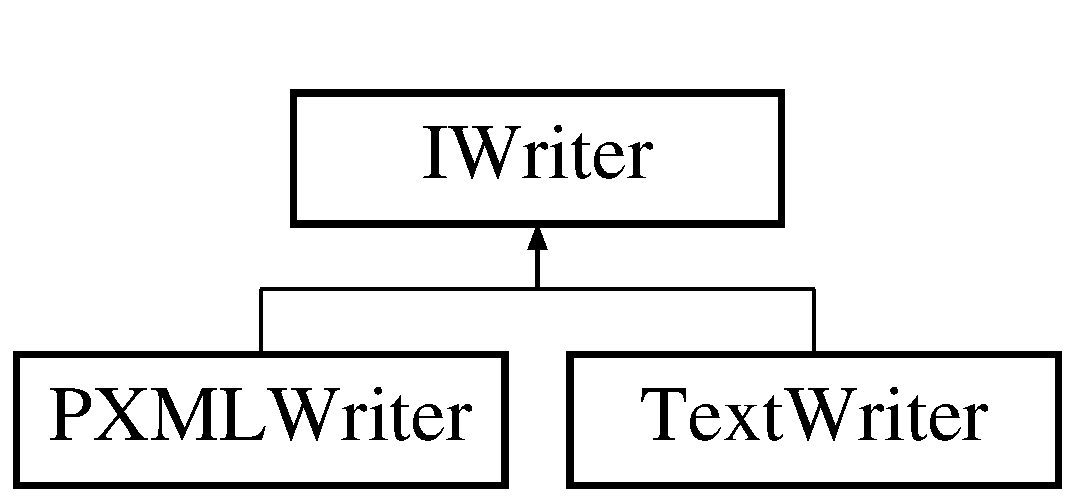
\includegraphics[height=2.000000cm]{interface_i_writer}
\end{center}
\end{figure}
\subsection*{Public Member Functions}
\begin{DoxyCompactItemize}
\item 
{\bf write} (\$message, \$level)
\end{DoxyCompactItemize}


\subsection{Member Function Documentation}
\index{I\-Writer@{I\-Writer}!write@{write}}
\index{write@{write}!IWriter@{I\-Writer}}
\subsubsection[{write}]{\setlength{\rightskip}{0pt plus 5cm}write (
\begin{DoxyParamCaption}
\item[{}]{\$message, }
\item[{}]{\$level}
\end{DoxyParamCaption}
)}\label{interface_i_writer_aecf647bb93e520f455d1145622b5db41}
write

Ajout d'un log


\begin{DoxyParams}{Parameters}
{\em string} & message log \\
\hline
{\em string} & level \\
\hline
\end{DoxyParams}


Implemented in {\bf Text\-Writer} \doxyref{}{p.}{class_text_writer_aecf647bb93e520f455d1145622b5db41}, and {\bf P\-X\-M\-L\-Writer} \doxyref{}{p.}{class_p_x_m_l_writer_aecf647bb93e520f455d1145622b5db41}.



The documentation for this interface was generated from the following file\-:\begin{DoxyCompactItemize}
\item 
D\-:/\-Documents/\-Git\-Hub/diapazen/system/\-L\-O\-G/I\-Writer.\-php\end{DoxyCompactItemize}

\section{Mail\-Util Class Reference}
\label{class_mail_util}\index{Mail\-Util@{Mail\-Util}}
\subsection*{Public Member Functions}
\begin{DoxyCompactItemize}
\item 
{\bf Mail\-Util} ()
\item 
{\bf send\-Mail} (\$mail\-To, \$subject, \$message)
\item 
{\bf send\-Mail\-With\-C\-C} (\$mails\-To, \$subjet, \$message)
\end{DoxyCompactItemize}
\subsection*{Protected Attributes}
\begin{DoxyCompactItemize}
\item 
{\bfseries \$mail\-From}\label{class_mail_util_a74d2bb596f6dd93248139a3c83b7000d}

\item 
{\bfseries \$name\-Mail\-From}\label{class_mail_util_aba7134dd951dd0e268449e124e264ccd}

\item 
{\bfseries \$pwd\-From}\label{class_mail_util_a40f8f3343b1d3e4b2a0f8608a76009f3}

\item 
{\bfseries \$config\-S\-M\-T\-P}\label{class_mail_util_ac69f81c310ffbe6815c58891082b22d1}

\end{DoxyCompactItemize}


\subsection{Member Function Documentation}
\index{Mail\-Util@{Mail\-Util}!Mail\-Util@{Mail\-Util}}
\index{Mail\-Util@{Mail\-Util}!MailUtil@{Mail\-Util}}
\subsubsection[{Mail\-Util}]{\setlength{\rightskip}{0pt plus 5cm}{\bf Mail\-Util} (
\begin{DoxyParamCaption}
{}
\end{DoxyParamCaption}
)}\label{class_mail_util_a46d3fa7fb5aaeba9ddeeea4165cf6dca}
Constructeur de \doxyref{Mail\-Util}{p.}{class_mail_util} \index{Mail\-Util@{Mail\-Util}!send\-Mail@{send\-Mail}}
\index{send\-Mail@{send\-Mail}!MailUtil@{Mail\-Util}}
\subsubsection[{send\-Mail}]{\setlength{\rightskip}{0pt plus 5cm}send\-Mail (
\begin{DoxyParamCaption}
\item[{}]{\$mail\-To, }
\item[{}]{\$subject, }
\item[{}]{\$message}
\end{DoxyParamCaption}
)}\label{class_mail_util_ae4692c91ee89d712a1b1918e56f4d46a}
Fonction permettant d'envoyer un mail

Cette méthode permet d'envoyer un mail depuis \$mail\-From à \$mail\-To


\begin{DoxyParams}[1]{Parameters}
string & {\em \$mail\-To} & mail de destination \\
\hline
string & {\em \$subject} & sujet du mail \\
\hline
string & {\em \$message} & message du mail \\
\hline
\end{DoxyParams}
\index{Mail\-Util@{Mail\-Util}!send\-Mail\-With\-C\-C@{send\-Mail\-With\-C\-C}}
\index{send\-Mail\-With\-C\-C@{send\-Mail\-With\-C\-C}!MailUtil@{Mail\-Util}}
\subsubsection[{send\-Mail\-With\-C\-C}]{\setlength{\rightskip}{0pt plus 5cm}send\-Mail\-With\-C\-C (
\begin{DoxyParamCaption}
\item[{}]{\$mails\-To, }
\item[{}]{\$subjet, }
\item[{}]{\$message}
\end{DoxyParamCaption}
)}\label{class_mail_util_ad6efaac390e560e95185d4e73a6ad850}
Fonction permettant d'envoyer un mail à plusieurs personne en copie carbone

Cette méthode permet d'envoyer un mail depuis \$mail\-From à \$mail\-To


\begin{DoxyParams}[1]{Parameters}
string & {\em \$mail\-To} & tableau des mails de destination \\
\hline
string & {\em \$subject} & sujet du mail \\
\hline
string & {\em \$message} & message du mail \\
\hline
\end{DoxyParams}


The documentation for this class was generated from the following file\-:\begin{DoxyCompactItemize}
\item 
D\-:/\-Documents/\-Git\-Hub/diapazen/util/Mail\-Util.\-class.\-php\end{DoxyCompactItemize}

\section{Message Class Reference}
\label{class_message}\index{Message@{Message}}
\subsection*{Public Member Functions}
\begin{DoxyCompactItemize}
\item 
{\bf get\-Message} ()
\item 
{\bf set\-Message} (\$name)
\item 
{\bf set\-Params} (\$params)
\end{DoxyCompactItemize}


\subsection{Member Function Documentation}
\index{Message@{Message}!get\-Message@{get\-Message}}
\index{get\-Message@{get\-Message}!Message@{Message}}
\subsubsection[{get\-Message}]{\setlength{\rightskip}{0pt plus 5cm}get\-Message (
\begin{DoxyParamCaption}
{}
\end{DoxyParamCaption}
)}\label{class_message_a0b0e611236742aac18ba1936d03ba89a}
Récupère le message à envoyer

\begin{DoxyReturn}{Returns}
string message à envoyer 
\end{DoxyReturn}
\index{Message@{Message}!set\-Message@{set\-Message}}
\index{set\-Message@{set\-Message}!Message@{Message}}
\subsubsection[{set\-Message}]{\setlength{\rightskip}{0pt plus 5cm}set\-Message (
\begin{DoxyParamCaption}
\item[{}]{\$name}
\end{DoxyParamCaption}
)}\label{class_message_aeaa3b32ef5d6eb86fdacbbefe383f750}
Récupère le message à envoyer

On utilise un switch sur '\$name' afin de savoir quel message récupérer


\begin{DoxyParams}{Parameters}
{\em name} & nom permettant de savoir quel message choisir \\
\hline
\end{DoxyParams}
\index{Message@{Message}!set\-Params@{set\-Params}}
\index{set\-Params@{set\-Params}!Message@{Message}}
\subsubsection[{set\-Params}]{\setlength{\rightskip}{0pt plus 5cm}set\-Params (
\begin{DoxyParamCaption}
\item[{}]{\$params}
\end{DoxyParamCaption}
)}\label{class_message_a99452a2ee9dfa3243a205c61d8f728cc}
Set les paramêtres des messages (ex \-: mot de passe)

Set les paramêtres des messages grâce à la fonction vsprintf Rajoute une ligne à la fin de tous les messages


\begin{DoxyParams}{Parameters}
{\em params} & tableau des paramêtres du message \\
\hline
\end{DoxyParams}


The documentation for this class was generated from the following file\-:\begin{DoxyCompactItemize}
\item 
D\-:/\-Documents/\-Git\-Hub/diapazen/util/Message.\-class.\-php\end{DoxyCompactItemize}

\section{Model Class Reference}
\label{class_model}\index{Model@{Model}}
Inheritance diagram for Model\-:\begin{figure}[H]
\begin{center}
\leavevmode
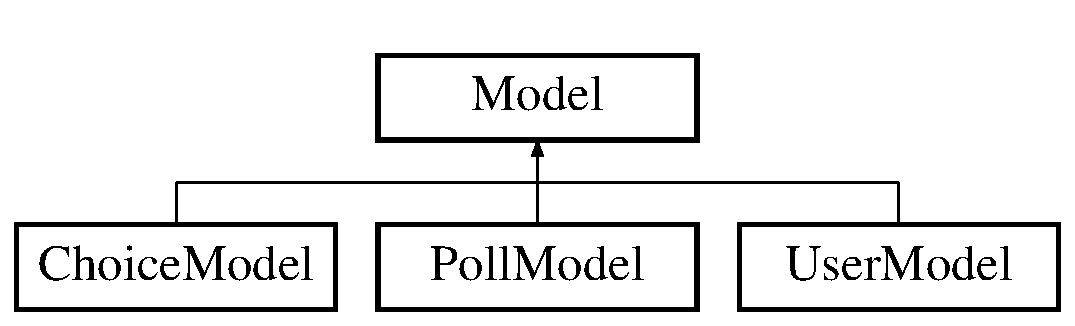
\includegraphics[height=2.000000cm]{class_model}
\end{center}
\end{figure}
\subsection*{Public Member Functions}
\begin{DoxyCompactItemize}
\item 
{\bf \-\_\-\-\_\-construct} ()
\item 
{\bf get\-P\-D\-O} ()
\item 
{\bf select} (\$fields, \$table, \$fetch\-Mode= 'both')
\item 
{\bf select\-Where} (\$fields, \$table, \$conditions, \$fetch\-Mode= 'both')
\item 
{\bf select\-Where\-Order\-By} (\$fields, \$table, \$conditions, \$orderby, \$fetch\-Mode= 'both')
\item 
{\bf insert} (\$values, \$table)
\item 
{\bf update\-Where} (\$values, \$conditions, \$table)
\item 
{\bf delete\-From} (\$conditions, \$table)
\end{DoxyCompactItemize}
\subsection*{Static Protected Attributes}
\begin{DoxyCompactItemize}
\item 
static {\bfseries \$m\-P\-D\-O}\label{class_model_a9c654cd1eac60f691cf2b4dbdfc0c4bd}

\end{DoxyCompactItemize}


\subsection{Constructor \& Destructor Documentation}
\index{Model@{Model}!\-\_\-\-\_\-construct@{\-\_\-\-\_\-construct}}
\index{\-\_\-\-\_\-construct@{\-\_\-\-\_\-construct}!Model@{Model}}
\subsubsection[{\-\_\-\-\_\-construct}]{\setlength{\rightskip}{0pt plus 5cm}\-\_\-\-\_\-construct (
\begin{DoxyParamCaption}
{}
\end{DoxyParamCaption}
)}\label{class_model_a095c5d389db211932136b53f25f39685}
Constructeur 

\subsection{Member Function Documentation}
\index{Model@{Model}!delete\-From@{delete\-From}}
\index{delete\-From@{delete\-From}!Model@{Model}}
\subsubsection[{delete\-From}]{\setlength{\rightskip}{0pt plus 5cm}delete\-From (
\begin{DoxyParamCaption}
\item[{}]{\$conditions, }
\item[{}]{\$table}
\end{DoxyParamCaption}
)}\label{class_model_af425d27609307a8678fbd649083bd94f}
Supprime un enregistrement de la table

Permet de réaliser une requête Delete sur la table '\$table' avec comme paramêtre '\$conditions'


\begin{DoxyParams}[1]{Parameters}
array & {\em \$conditions} & Un tableau A\-S\-S\-O\-C\-I\-A\-T\-I\-F des conditions \\
\hline
string & {\em \$table} & Table de la base de données\\
\hline
\end{DoxyParams}
\begin{DoxyReturn}{Returns}
Vrai si réussite sinon Faux 
\end{DoxyReturn}
\index{Model@{Model}!get\-P\-D\-O@{get\-P\-D\-O}}
\index{get\-P\-D\-O@{get\-P\-D\-O}!Model@{Model}}
\subsubsection[{get\-P\-D\-O}]{\setlength{\rightskip}{0pt plus 5cm}get\-P\-D\-O (
\begin{DoxyParamCaption}
{}
\end{DoxyParamCaption}
)}\label{class_model_af708fa20ff0c04a5a9bd8badd63e632c}
Récupère l'instance de P\-D\-O

\begin{DoxyReturn}{Returns}
Instance de P\-D\-O 
\end{DoxyReturn}
\index{Model@{Model}!insert@{insert}}
\index{insert@{insert}!Model@{Model}}
\subsubsection[{insert}]{\setlength{\rightskip}{0pt plus 5cm}insert (
\begin{DoxyParamCaption}
\item[{}]{\$values, }
\item[{}]{\$table}
\end{DoxyParamCaption}
)}\label{class_model_a8c4aa25cad6375a8a41f4d822aad70de}
Insère des données dans la base de données


\begin{DoxyParams}[1]{Parameters}
array & {\em \$values} & Tableau A\-S\-S\-O\-C\-I\-A\-T\-I\-F des valeurs à insérer \\
\hline
string & {\em \$table} & Table de la base de données\\
\hline
\end{DoxyParams}
\begin{DoxyReturn}{Returns}
Vrai si réussite sinon Faux 
\end{DoxyReturn}
\index{Model@{Model}!select@{select}}
\index{select@{select}!Model@{Model}}
\subsubsection[{select}]{\setlength{\rightskip}{0pt plus 5cm}select (
\begin{DoxyParamCaption}
\item[{}]{\$fields, }
\item[{}]{\$table, }
\item[{}]{\$fetch\-Mode = {\ttfamily 'both'}}
\end{DoxyParamCaption}
)}\label{class_model_a4a144616f9727cd503fb5fb117ea9e9a}
Récupère des informations d'une table ou d'une vue de la base de données.

Permet de réaliser une requête Select simple sur la table '\$table' et qui retourne les paramêtres '\$fields' On peut choisir le type fetch de retour \-: assoc ou num (par défaut both)


\begin{DoxyParams}[1]{Parameters}
array | string & {\em \$fields} & Champs de la table \\
\hline
string & {\em \$table} & Table de la base de données \\
\hline
type & {\em \$fetch\-Mode} & Permet de choisir quel 'fetch' utiliser par défaut 'both'\\
\hline
\end{DoxyParams}
\begin{DoxyReturn}{Returns}
Un tableau de résultats 
\end{DoxyReturn}
\index{Model@{Model}!select\-Where@{select\-Where}}
\index{select\-Where@{select\-Where}!Model@{Model}}
\subsubsection[{select\-Where}]{\setlength{\rightskip}{0pt plus 5cm}select\-Where (
\begin{DoxyParamCaption}
\item[{}]{\$fields, }
\item[{}]{\$table, }
\item[{}]{\$conditions, }
\item[{}]{\$fetch\-Mode = {\ttfamily 'both'}}
\end{DoxyParamCaption}
)}\label{class_model_ad3544d723ab065f4acd12e52c28336da}
Récupère des informations d'une table ou d'une vue de la base de données.

Permet de réaliser une requête Select sur la table '\$table' avec comme paramêtre '\$conditions' et qui retourne les paramêtres '\$fields' On peut choisir le type fetch de retour \-: assoc ou num (par défaut both)


\begin{DoxyParams}[1]{Parameters}
array | string & {\em \$fields} & Champs de la table \\
\hline
string & {\em \$table} & Table de la base de données \\
\hline
array & {\em \$conditions} & Un tableau A\-S\-S\-O\-C\-I\-A\-T\-I\-F des conditions \\
\hline
type & {\em \$fetch\-Mode} & Permet de choisir quel 'fetch' utiliser par défaut 'both'\\
\hline
\end{DoxyParams}
\begin{DoxyReturn}{Returns}
Un tableau de résultats 
\end{DoxyReturn}
\index{Model@{Model}!select\-Where\-Order\-By@{select\-Where\-Order\-By}}
\index{select\-Where\-Order\-By@{select\-Where\-Order\-By}!Model@{Model}}
\subsubsection[{select\-Where\-Order\-By}]{\setlength{\rightskip}{0pt plus 5cm}select\-Where\-Order\-By (
\begin{DoxyParamCaption}
\item[{}]{\$fields, }
\item[{}]{\$table, }
\item[{}]{\$conditions, }
\item[{}]{\$orderby, }
\item[{}]{\$fetch\-Mode = {\ttfamily 'both'}}
\end{DoxyParamCaption}
)}\label{class_model_a36ca044fc8dd4808f6c6206d2cfc4d62}
Récupère des informations d'une table ou d'une vue de la base de données.

Permet de réaliser une requête Select sur la table '\$table' avec comme paramêtre '\$conditions' et les ordonnant avec 'orderby' et qui retourne les paramêtres '\$fields' On peut choisir le type fetch de retour \-: assoc ou num (par défaut both)


\begin{DoxyParams}[1]{Parameters}
array | string & {\em \$fields} & Champs de la table \\
\hline
string & {\em \$table} & Table de la base de données \\
\hline
array & {\em \$conditions} & Un tableau A\-S\-S\-O\-C\-I\-A\-T\-I\-F des conditions \\
\hline
array & {\em \$orderby} & Un tableau ex\-: array('nom desc', 'prenom asc') \\
\hline
type & {\em \$fetch\-Mode} & Permet de choisir quel 'fetch' utiliser par défaut 'both'\\
\hline
\end{DoxyParams}
\begin{DoxyReturn}{Returns}
Un tableau de résultats 
\end{DoxyReturn}
\index{Model@{Model}!update\-Where@{update\-Where}}
\index{update\-Where@{update\-Where}!Model@{Model}}
\subsubsection[{update\-Where}]{\setlength{\rightskip}{0pt plus 5cm}update\-Where (
\begin{DoxyParamCaption}
\item[{}]{\$values, }
\item[{}]{\$conditions, }
\item[{}]{\$table}
\end{DoxyParamCaption}
)}\label{class_model_aeac063e0a8b8048310967c496cb7d561}
Met à jour un enregistrement de la table

Permet de réaliser une requête Update sur la table '\$table' avec comme paramêtre '\$conditions' et qui met à jour avec '\$values'


\begin{DoxyParams}[1]{Parameters}
array & {\em \$values} & Un tableau A\-S\-S\-O\-C\-I\-A\-T\-I\-F des valeurs \\
\hline
array & {\em \$conditions} & Un tableau A\-S\-S\-O\-C\-I\-A\-T\-I\-F des conditions \\
\hline
string & {\em \$table} & Table de la base de données\\
\hline
\end{DoxyParams}
\begin{DoxyReturn}{Returns}
Vrai si réussite sinon Faux 
\end{DoxyReturn}


The documentation for this class was generated from the following file\-:\begin{DoxyCompactItemize}
\item 
D\-:/\-Documents/\-Git\-Hub/diapazen/system/Model.\-class.\-php\end{DoxyCompactItemize}

\section{Number\-Util Class Reference}
\label{class_number_util}\index{Number\-Util@{Number\-Util}}
\subsection*{Static Public Member Functions}
\begin{DoxyCompactItemize}
\item 
static {\bf get\-Pourcentage} (\$number, \$total)
\item 
static {\bf get\-Number\-With\-Percentage} (\$number, \$percent)
\end{DoxyCompactItemize}


\subsection{Member Function Documentation}
\index{Number\-Util@{Number\-Util}!get\-Number\-With\-Percentage@{get\-Number\-With\-Percentage}}
\index{get\-Number\-With\-Percentage@{get\-Number\-With\-Percentage}!NumberUtil@{Number\-Util}}
\subsubsection[{get\-Number\-With\-Percentage}]{\setlength{\rightskip}{0pt plus 5cm}static get\-Number\-With\-Percentage (
\begin{DoxyParamCaption}
\item[{}]{\$number, }
\item[{}]{\$percent}
\end{DoxyParamCaption}
)\hspace{0.3cm}{\ttfamily [static]}}\label{class_number_util_af89b340bcdf29694ceb39868d7e7c959}
Donne le nombre apres application d'un pourcentage


\begin{DoxyParams}[1]{Parameters}
int & {\em \$number} & nombre d'element de base \\
\hline
int & {\em \$percent} & le pourcentage a appliquer \\
\hline
\end{DoxyParams}
\begin{DoxyReturn}{Returns}
int le nouveau nombre 
\end{DoxyReturn}
\index{Number\-Util@{Number\-Util}!get\-Pourcentage@{get\-Pourcentage}}
\index{get\-Pourcentage@{get\-Pourcentage}!NumberUtil@{Number\-Util}}
\subsubsection[{get\-Pourcentage}]{\setlength{\rightskip}{0pt plus 5cm}static get\-Pourcentage (
\begin{DoxyParamCaption}
\item[{}]{\$number, }
\item[{}]{\$total}
\end{DoxyParamCaption}
)\hspace{0.3cm}{\ttfamily [static]}}\label{class_number_util_a6454e7cb412078d9d139ab0643233fe6}
Donne le pourcentage de valeur avec arrondi


\begin{DoxyParams}[1]{Parameters}
int & {\em \$number} & nombre d'element \\
\hline
int & {\em \$total} & nombre d'element total \\
\hline
\end{DoxyParams}
\begin{DoxyReturn}{Returns}
int le pourcentage 
\end{DoxyReturn}


The documentation for this class was generated from the following file\-:\begin{DoxyCompactItemize}
\item 
D\-:/\-Documents/\-Git\-Hub/diapazen/util/Number\-Util.\-class.\-php\end{DoxyCompactItemize}

\section{Poll\-Controller Class Reference}
\label{class_poll_controller}\index{Poll\-Controller@{Poll\-Controller}}
Inheritance diagram for Poll\-Controller\-:\begin{figure}[H]
\begin{center}
\leavevmode
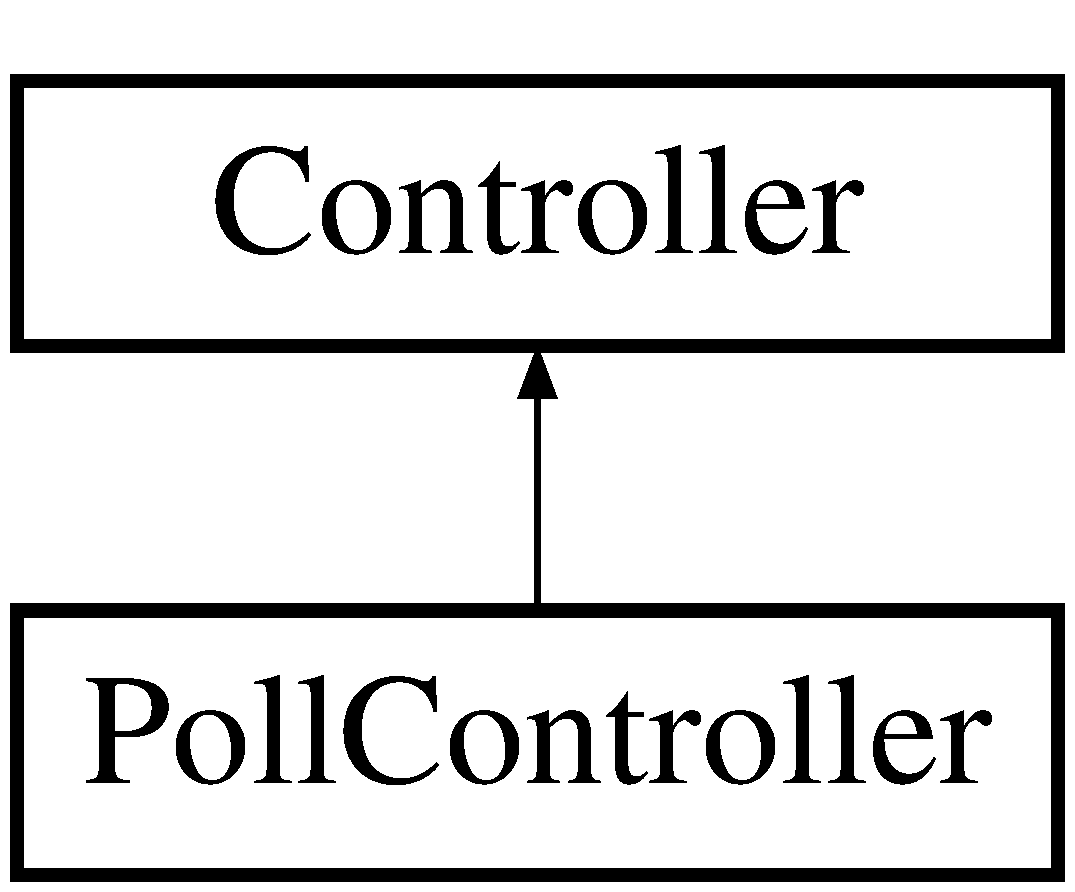
\includegraphics[height=2.000000cm]{class_poll_controller}
\end{center}
\end{figure}
\subsection*{Public Member Functions}
\begin{DoxyCompactItemize}
\item 
{\bf index} (\$params=null)
\item 
{\bf create} (\$params=null)
\item 
{\bf connect} (\$params=null)
\item 
{\bf share} (\$params=null)
\item 
{\bf sent} (\$params=null)
\item 
{\bf view} (\$params=null)
\end{DoxyCompactItemize}
\subsection*{Additional Inherited Members}


\subsection{Member Function Documentation}
\index{Poll\-Controller@{Poll\-Controller}!connect@{connect}}
\index{connect@{connect}!PollController@{Poll\-Controller}}
\subsubsection[{connect}]{\setlength{\rightskip}{0pt plus 5cm}connect (
\begin{DoxyParamCaption}
\item[{}]{\$params = {\ttfamily null}}
\end{DoxyParamCaption}
)}\label{class_poll_controller_aef0c1d8cc930dc55039b74f6d1a4bbb3}
Page connec lors de la création d'un sondage

Gère \-:
\begin{DoxyItemize}
\item Met le titre de la page à 'Création d\textbackslash{}'un sondage $|$ \doxyref{Diapazen}{p.}{namespace_diapazen}'.
\item Renvoi à la partie create si on y a pas été
\item Envoi directement l'utilisateur à la partie 'partage' si il est déjà connecté
\item Si on est déjà inscrit on tente de se connecter
\item Si on n'est pas inscrit, on inscrit l'utilisateur et on lui envoi un mail avec son mot de passe
\item Gère si des erreurs sont survenues
\end{DoxyItemize}


\begin{DoxyParams}[1]{Parameters}
type & {\em \$params} & null par défaut \\
\hline
\end{DoxyParams}
\index{Poll\-Controller@{Poll\-Controller}!create@{create}}
\index{create@{create}!PollController@{Poll\-Controller}}
\subsubsection[{create}]{\setlength{\rightskip}{0pt plus 5cm}create (
\begin{DoxyParamCaption}
\item[{}]{\$params = {\ttfamily null}}
\end{DoxyParamCaption}
)}\label{class_poll_controller_ad4a15717b6326aeddf9e36a4e578fc62}
Création d'un sondage

Gère \-:
\begin{DoxyItemize}
\item Lance le render de la vue 'poll\-Creation'
\item Met le titre de la page à 'Création d\textbackslash{}'un sondage $|$ \doxyref{Diapazen}{p.}{namespace_diapazen}'.
\item Récupère les renseignements donnés si on fait 'précédent'
\end{DoxyItemize}


\begin{DoxyParams}[1]{Parameters}
type & {\em \$params} & null par défaut \\
\hline
\end{DoxyParams}
\index{Poll\-Controller@{Poll\-Controller}!index@{index}}
\index{index@{index}!PollController@{Poll\-Controller}}
\subsubsection[{index}]{\setlength{\rightskip}{0pt plus 5cm}index (
\begin{DoxyParamCaption}
\item[{}]{\$params = {\ttfamily null}}
\end{DoxyParamCaption}
)}\label{class_poll_controller_a749de566b023589025bfebbc37537d65}
Index des sondages

Lance la méthode 'create' de \doxyref{Poll\-Controller}{p.}{class_poll_controller}


\begin{DoxyParams}[1]{Parameters}
type & {\em \$params} & null par défaut \\
\hline
\end{DoxyParams}
\index{Poll\-Controller@{Poll\-Controller}!sent@{sent}}
\index{sent@{sent}!PollController@{Poll\-Controller}}
\subsubsection[{sent}]{\setlength{\rightskip}{0pt plus 5cm}sent (
\begin{DoxyParamCaption}
\item[{}]{\$params = {\ttfamily null}}
\end{DoxyParamCaption}
)}\label{class_poll_controller_a62467d03c837586c4708d1b21d0120b7}
Partage d'un sondage

Gère \-:
\begin{DoxyItemize}
\item Met le titre de la page à 'Création d\textbackslash{}'un sondage $|$ \doxyref{Diapazen}{p.}{namespace_diapazen}'.
\item Renvoi à la page d'accueil si nous ne venons pas créer un sondage
\item Envois des mails de partage au mails spécifiés
\item Lance le render de la vue 'share\-Mail'
\item Gère si des erreurs sont survenues
\end{DoxyItemize}


\begin{DoxyParams}[1]{Parameters}
type & {\em \$params} & null par défaut \\
\hline
\end{DoxyParams}
\index{Poll\-Controller@{Poll\-Controller}!share@{share}}
\index{share@{share}!PollController@{Poll\-Controller}}
\subsubsection[{share}]{\setlength{\rightskip}{0pt plus 5cm}share (
\begin{DoxyParamCaption}
\item[{}]{\$params = {\ttfamily null}}
\end{DoxyParamCaption}
)}\label{class_poll_controller_adc75f0e1d90a818ec6f956f0bea0506f}
Partage d'un sondage

Gère \-:
\begin{DoxyItemize}
\item Met le titre de la page à 'Création d\textbackslash{}'un sondage $|$ \doxyref{Diapazen}{p.}{namespace_diapazen}'.
\item Renvoi à la partie create si on y a pas été
\item Ajoute le sondage dans la base de donnée
\item Ajoute les choix dans la base de donnée
\item Lance le render de la vue 'poll\-Share'
\item Gère si des erreurs sont survenues
\end{DoxyItemize}


\begin{DoxyParams}[1]{Parameters}
type & {\em \$params} & null par défaut \\
\hline
\end{DoxyParams}
\index{Poll\-Controller@{Poll\-Controller}!view@{view}}
\index{view@{view}!PollController@{Poll\-Controller}}
\subsubsection[{view}]{\setlength{\rightskip}{0pt plus 5cm}view (
\begin{DoxyParamCaption}
\item[{}]{\$params = {\ttfamily null}}
\end{DoxyParamCaption}
)}\label{class_poll_controller_af05c3382fc723fd84e5d49c18af43913}
Visualisation d'un sondage

Gère \-:
\begin{DoxyItemize}
\item Met le titre de la page à 'Création d\textbackslash{}'un sondage $|$ \doxyref{Diapazen}{p.}{namespace_diapazen}'.
\item Renvoi à la page d'accueil si l'url du sondage n'est pas specifiée
\item Renvoi un 404 si le sondage n'a pas été trouvé
\item Empêche le revote grâce à la fonction 'rafraichir la page'
\item L'ajout de vote dans le sondage
\item Trie les choix en fonction des résultats pour un sondage fermé
\item Affiche qui a voté quoi
\item Lance le render de la vue 'poll\-View'
\item Gère si des erreurs sont survenues
\end{DoxyItemize}


\begin{DoxyParams}[1]{Parameters}
type & {\em \$params} & null par défaut \\
\hline
\end{DoxyParams}


The documentation for this class was generated from the following file\-:\begin{DoxyCompactItemize}
\item 
D\-:/\-Documents/\-Git\-Hub/diapazen/app/controller/Poll\-Controller.\-class.\-php\end{DoxyCompactItemize}

\section{Poll\-Model Class Reference}
\label{class_poll_model}\index{Poll\-Model@{Poll\-Model}}
Inheritance diagram for Poll\-Model\-:\begin{figure}[H]
\begin{center}
\leavevmode
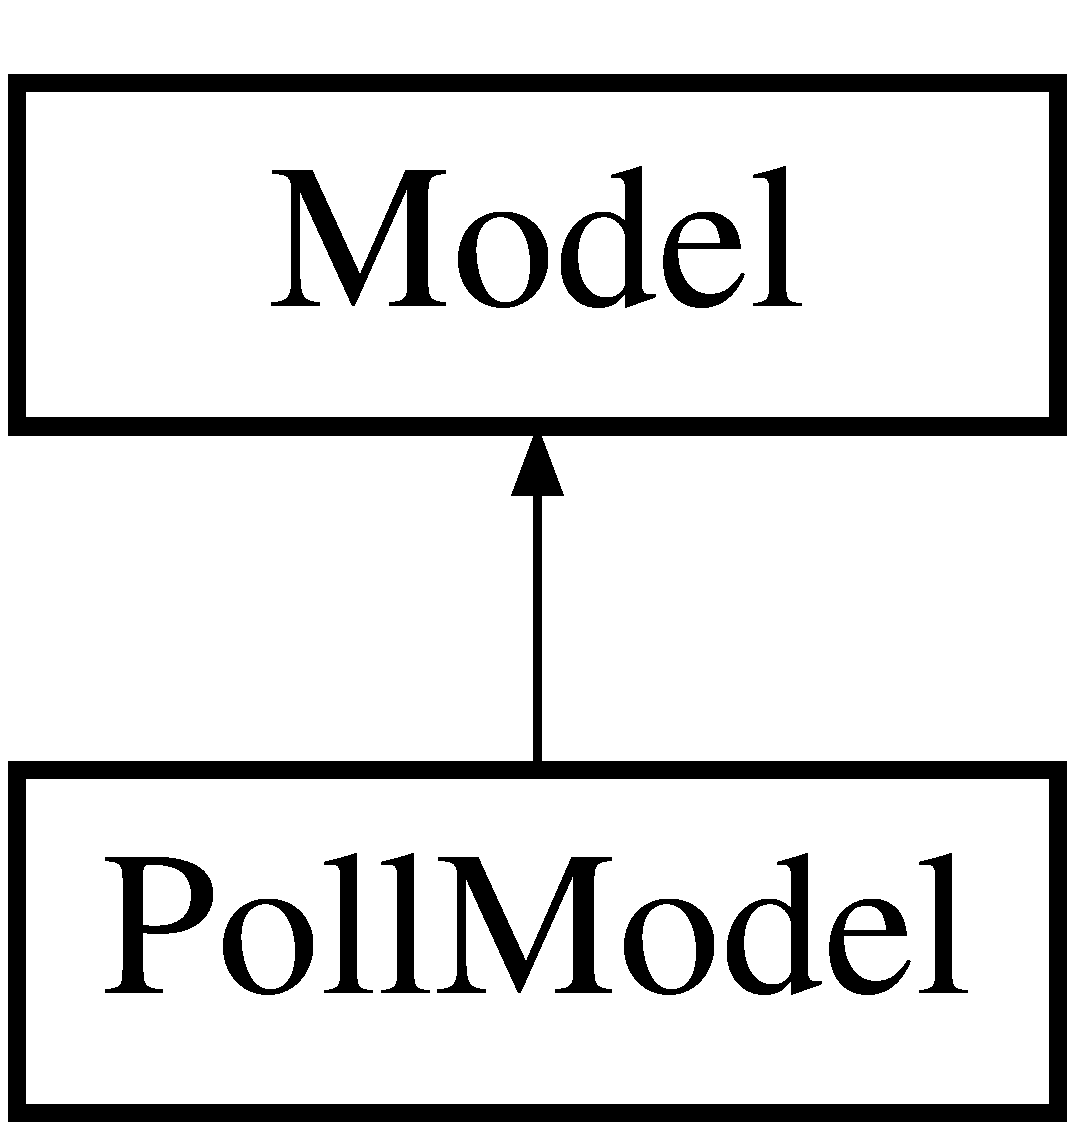
\includegraphics[height=2.000000cm]{class_poll_model}
\end{center}
\end{figure}
\subsection*{Public Member Functions}
\begin{DoxyCompactItemize}
\item 
{\bf \-\_\-\-\_\-construct} ()
\item 
{\bf view\-Poll} (\$poll\-Url)
\item 
{\bf view\-All\-Polls} (\$user\-Id)
\item 
{\bf add\-Poll} (\$user\-Id, \$poll\-Title, \$poll\-Description, \$poll\-\_\-expiration\-\_\-date)
\item 
{\bf vote\-Poll} (\$choice\-Id, \$value)
\item 
{\bf update\-Poll} (\$poll\-Id)
\item 
{\bf share\-Poll} (\$textearea\-Content)
\item 
{\bf set\-Poll\-Title} (\$poll\-Title)
\item 
{\bf set\-Poll\-Id} (\$poll\-Id)
\item 
{\bf set\-Poll\-Description} (\$poll\-Description)
\item 
{\bf set\-Poll\-Expiration\-Date} (\$poll\-\_\-expiration\-\_\-date)
\item 
{\bf set\-Poll\-Url} (\$poll\-Url)
\item 
{\bf get\-Poll\-Id} ()
\item 
{\bf get\-Poll\-Title} ()
\item 
{\bf get\-Poll\-Description} ()
\item 
{\bf get\-Poll\-Expiration\-Date} ()
\item 
{\bf get\-Poll\-Url} ()
\end{DoxyCompactItemize}
\subsection*{Additional Inherited Members}


\subsection{Constructor \& Destructor Documentation}
\index{Poll\-Model@{Poll\-Model}!\-\_\-\-\_\-construct@{\-\_\-\-\_\-construct}}
\index{\-\_\-\-\_\-construct@{\-\_\-\-\_\-construct}!PollModel@{Poll\-Model}}
\subsubsection[{\-\_\-\-\_\-construct}]{\setlength{\rightskip}{0pt plus 5cm}\-\_\-\-\_\-construct (
\begin{DoxyParamCaption}
{}
\end{DoxyParamCaption}
)}\label{class_poll_model_a095c5d389db211932136b53f25f39685}
Constructeur par d�faut 

\subsection{Member Function Documentation}
\index{Poll\-Model@{Poll\-Model}!add\-Poll@{add\-Poll}}
\index{add\-Poll@{add\-Poll}!PollModel@{Poll\-Model}}
\subsubsection[{add\-Poll}]{\setlength{\rightskip}{0pt plus 5cm}add\-Poll (
\begin{DoxyParamCaption}
\item[{}]{\$user\-Id, }
\item[{}]{\$poll\-Title, }
\item[{}]{\$poll\-Description, }
\item[{}]{\$poll\-\_\-expiration\-\_\-date}
\end{DoxyParamCaption}
)}\label{class_poll_model_af3934538e9ecfaab4c57c99eb3c27b41}
Ajout d'un sondage On commence par affecter les valeurs des propri�t�s de l�objet et on ajoute la ligne correspondante � la base de donn�es. 
\begin{DoxyParams}[1]{Parameters}
type & {\em \$user\-Id} & id de l'utilisateur \\
\hline
type & {\em \$poll\-Title} & titre du sondage \\
\hline
type & {\em \$poll\-Description} & description du sondage \\
\hline
type & {\em \$poll\-\_\-expiration\-\_\-date} & date d'expiration du sondage \\
\hline
\end{DoxyParams}
\begin{DoxyReturn}{Returns}
boolean true si l'ajout s'est bien ex�cut� sinon false 
\end{DoxyReturn}
\index{Poll\-Model@{Poll\-Model}!get\-Poll\-Description@{get\-Poll\-Description}}
\index{get\-Poll\-Description@{get\-Poll\-Description}!PollModel@{Poll\-Model}}
\subsubsection[{get\-Poll\-Description}]{\setlength{\rightskip}{0pt plus 5cm}get\-Poll\-Description (
\begin{DoxyParamCaption}
{}
\end{DoxyParamCaption}
)}\label{class_poll_model_a2a9c8903e596a9545465e5de17db0dfc}
Getteur de la description du sondage \index{Poll\-Model@{Poll\-Model}!get\-Poll\-Expiration\-Date@{get\-Poll\-Expiration\-Date}}
\index{get\-Poll\-Expiration\-Date@{get\-Poll\-Expiration\-Date}!PollModel@{Poll\-Model}}
\subsubsection[{get\-Poll\-Expiration\-Date}]{\setlength{\rightskip}{0pt plus 5cm}get\-Poll\-Expiration\-Date (
\begin{DoxyParamCaption}
{}
\end{DoxyParamCaption}
)}\label{class_poll_model_ac1e26034a3ac51c188cd1d903747bf08}
Getteur de la date d'expiration du sondage \index{Poll\-Model@{Poll\-Model}!get\-Poll\-Id@{get\-Poll\-Id}}
\index{get\-Poll\-Id@{get\-Poll\-Id}!PollModel@{Poll\-Model}}
\subsubsection[{get\-Poll\-Id}]{\setlength{\rightskip}{0pt plus 5cm}get\-Poll\-Id (
\begin{DoxyParamCaption}
{}
\end{DoxyParamCaption}
)}\label{class_poll_model_a55f7df314c542c220c7d19bc6bfe6921}
Getteur du titre du sondage \index{Poll\-Model@{Poll\-Model}!get\-Poll\-Title@{get\-Poll\-Title}}
\index{get\-Poll\-Title@{get\-Poll\-Title}!PollModel@{Poll\-Model}}
\subsubsection[{get\-Poll\-Title}]{\setlength{\rightskip}{0pt plus 5cm}get\-Poll\-Title (
\begin{DoxyParamCaption}
{}
\end{DoxyParamCaption}
)}\label{class_poll_model_ac53f9f9366ccd0ee4c493f8d9585641c}
Getteur de l'id du sondage \index{Poll\-Model@{Poll\-Model}!get\-Poll\-Url@{get\-Poll\-Url}}
\index{get\-Poll\-Url@{get\-Poll\-Url}!PollModel@{Poll\-Model}}
\subsubsection[{get\-Poll\-Url}]{\setlength{\rightskip}{0pt plus 5cm}get\-Poll\-Url (
\begin{DoxyParamCaption}
{}
\end{DoxyParamCaption}
)}\label{class_poll_model_a59162fd7493193e799f6d85318904f3d}
Getteur de l'url du sondage \index{Poll\-Model@{Poll\-Model}!set\-Poll\-Description@{set\-Poll\-Description}}
\index{set\-Poll\-Description@{set\-Poll\-Description}!PollModel@{Poll\-Model}}
\subsubsection[{set\-Poll\-Description}]{\setlength{\rightskip}{0pt plus 5cm}set\-Poll\-Description (
\begin{DoxyParamCaption}
\item[{}]{\$poll\-Description}
\end{DoxyParamCaption}
)}\label{class_poll_model_a23a8113e19599e2b1783baf00680e7c5}
Setteur de la description du sondage 
\begin{DoxyParams}[1]{Parameters}
type & {\em \$poll\-Description} & description du sondage \\
\hline
\end{DoxyParams}
\index{Poll\-Model@{Poll\-Model}!set\-Poll\-Expiration\-Date@{set\-Poll\-Expiration\-Date}}
\index{set\-Poll\-Expiration\-Date@{set\-Poll\-Expiration\-Date}!PollModel@{Poll\-Model}}
\subsubsection[{set\-Poll\-Expiration\-Date}]{\setlength{\rightskip}{0pt plus 5cm}set\-Poll\-Expiration\-Date (
\begin{DoxyParamCaption}
\item[{}]{\$poll\-\_\-expiration\-\_\-date}
\end{DoxyParamCaption}
)}\label{class_poll_model_a1cea7eb81f3cc7b83135712f1870f6ac}
Setteur de la date d'expiration du sondage 
\begin{DoxyParams}[1]{Parameters}
type & {\em \$poll\-\_\-expiration\-\_\-date} & date d'expiration du sondage \\
\hline
\end{DoxyParams}
\index{Poll\-Model@{Poll\-Model}!set\-Poll\-Id@{set\-Poll\-Id}}
\index{set\-Poll\-Id@{set\-Poll\-Id}!PollModel@{Poll\-Model}}
\subsubsection[{set\-Poll\-Id}]{\setlength{\rightskip}{0pt plus 5cm}set\-Poll\-Id (
\begin{DoxyParamCaption}
\item[{}]{\$poll\-Id}
\end{DoxyParamCaption}
)}\label{class_poll_model_a2fafeb8f9432d4d6f293c2662e2e3ce4}
Setteur de l'id du sondage 
\begin{DoxyParams}[1]{Parameters}
type & {\em \$poll\-Id} & Id du sondage \\
\hline
\end{DoxyParams}
\index{Poll\-Model@{Poll\-Model}!set\-Poll\-Title@{set\-Poll\-Title}}
\index{set\-Poll\-Title@{set\-Poll\-Title}!PollModel@{Poll\-Model}}
\subsubsection[{set\-Poll\-Title}]{\setlength{\rightskip}{0pt plus 5cm}set\-Poll\-Title (
\begin{DoxyParamCaption}
\item[{}]{\$poll\-Title}
\end{DoxyParamCaption}
)}\label{class_poll_model_a4ef3e29c3777e4813e34a426d4d4e5e5}
Setteur du titre du sondage 
\begin{DoxyParams}[1]{Parameters}
type & {\em \$poll\-Title} & titre du sondage \\
\hline
\end{DoxyParams}
\index{Poll\-Model@{Poll\-Model}!set\-Poll\-Url@{set\-Poll\-Url}}
\index{set\-Poll\-Url@{set\-Poll\-Url}!PollModel@{Poll\-Model}}
\subsubsection[{set\-Poll\-Url}]{\setlength{\rightskip}{0pt plus 5cm}set\-Poll\-Url (
\begin{DoxyParamCaption}
\item[{}]{\$poll\-Url}
\end{DoxyParamCaption}
)}\label{class_poll_model_a9fb57052af60b04cc3f9a5f6c63826b3}
Setteur de l'url du sondage 
\begin{DoxyParams}[1]{Parameters}
type & {\em \$poll\-Url} & url du sondage \\
\hline
\end{DoxyParams}
\index{Poll\-Model@{Poll\-Model}!share\-Poll@{share\-Poll}}
\index{share\-Poll@{share\-Poll}!PollModel@{Poll\-Model}}
\subsubsection[{share\-Poll}]{\setlength{\rightskip}{0pt plus 5cm}share\-Poll (
\begin{DoxyParamCaption}
\item[{}]{\$textearea\-Content}
\end{DoxyParamCaption}
)}\label{class_poll_model_a947a4723935496599a5c9f16dd923545}
R�cup�re le contenu du textarea et parse les emails au moyen d'une regexp. Elle retourne un tableau avec les email si le parsage est r�ussi et null sinon. 
\begin{DoxyParams}{Parameters}
{\em \$textearea\-Content} & \\
\hline
\end{DoxyParams}
\begin{DoxyReturn}{Returns}
Tableau avec les emails valides auquels les mails ont �t� envoy� 
\end{DoxyReturn}
\index{Poll\-Model@{Poll\-Model}!update\-Poll@{update\-Poll}}
\index{update\-Poll@{update\-Poll}!PollModel@{Poll\-Model}}
\subsubsection[{update\-Poll}]{\setlength{\rightskip}{0pt plus 5cm}update\-Poll (
\begin{DoxyParamCaption}
\item[{}]{\$poll\-Id}
\end{DoxyParamCaption}
)}\label{class_poll_model_a67c4aa7fb79831e0e6401e72974671d9}
Mise � jour de la table Sondage clos le sondage en mettant � 0 dans la colonne open de la table du sondage. \begin{DoxyReturn}{Returns}
boolean true si la mise � jour s'est bien ex�cut� sinon false 
\end{DoxyReturn}
\index{Poll\-Model@{Poll\-Model}!view\-All\-Polls@{view\-All\-Polls}}
\index{view\-All\-Polls@{view\-All\-Polls}!PollModel@{Poll\-Model}}
\subsubsection[{view\-All\-Polls}]{\setlength{\rightskip}{0pt plus 5cm}view\-All\-Polls (
\begin{DoxyParamCaption}
\item[{}]{\$user\-Id}
\end{DoxyParamCaption}
)}\label{class_poll_model_a3aa12da9f991255d673ee280b6b4608c}
Affichage de la liste des sondages cr�� par l�utilisateur en prenant en param�tre l�\-Id de l�utilisateur avec une requ�te select sur la vue dpz\-\_\-view\-\_\-users\-\_\-join\-\_\-polls. 
\begin{DoxyParams}[1]{Parameters}
type & {\em \$poll\-Url} & url du sondage \\
\hline
\end{DoxyParams}
\begin{DoxyReturn}{Returns}
array contenu du sondage 
\end{DoxyReturn}
\index{Poll\-Model@{Poll\-Model}!view\-Poll@{view\-Poll}}
\index{view\-Poll@{view\-Poll}!PollModel@{Poll\-Model}}
\subsubsection[{view\-Poll}]{\setlength{\rightskip}{0pt plus 5cm}view\-Poll (
\begin{DoxyParamCaption}
\item[{}]{\$poll\-Url}
\end{DoxyParamCaption}
)}\label{class_poll_model_a59ebd496c5314a98f881b3017ac5e831}
Affichage d'un sondage en r�cup�rant les informations stock�es dans la base de donn�es au moyen d�une requ�te sql Select sur la vue dpz\-\_\-view\-\_\-users\-\_\-join\-\_\-polls. On traite le r�sultat obtenu en r�cup�rant les informations de chaque choix du sondage ainsi que les informations de chaque r�sultat des choix du sondage. Les r�sultats obtenus sont ensuite transf�r�s dans un tableau et on calcule le pourcentage de chaque choix du sondage. Le tableau est donc compl�t� avec ces m�mes pourcentages. 
\begin{DoxyParams}[1]{Parameters}
type & {\em \$poll\-Url} & url du sondage \\
\hline
\end{DoxyParams}
\begin{DoxyReturn}{Returns}
array contenu du sondage 
\end{DoxyReturn}
\index{Poll\-Model@{Poll\-Model}!vote\-Poll@{vote\-Poll}}
\index{vote\-Poll@{vote\-Poll}!PollModel@{Poll\-Model}}
\subsubsection[{vote\-Poll}]{\setlength{\rightskip}{0pt plus 5cm}vote\-Poll (
\begin{DoxyParamCaption}
\item[{}]{\$choice\-Id, }
\item[{}]{\$value}
\end{DoxyParamCaption}
)}\label{class_poll_model_a25cacb3dabfcb04e5d45b50c7fc74a8f}
Vote d'un sondage pour le choix du sondage gr�ce � l�\-Id du choix et la valeur du votant. On ins�re cette ligne dans la base de donn�es, dans la table dpz\-\_\-results. 
\begin{DoxyParams}[1]{Parameters}
int & {\em \$choice\-Id} & L'id du choix \\
\hline
string & {\em \$poll\-Title} & valeur � ins�rer \\
\hline
\end{DoxyParams}
\begin{DoxyReturn}{Returns}
boolean true si l'ajout s'est bien ex�cut� sinon false 
\end{DoxyReturn}


The documentation for this class was generated from the following file\-:\begin{DoxyCompactItemize}
\item 
D\-:/\-Documents/\-Git\-Hub/diapazen/app/model/Poll\-Model.\-class.\-php\end{DoxyCompactItemize}

\section{P\-X\-M\-L\-Writer Class Reference}
\label{class_p_x_m_l_writer}\index{P\-X\-M\-L\-Writer@{P\-X\-M\-L\-Writer}}
Inheritance diagram for P\-X\-M\-L\-Writer\-:\begin{figure}[H]
\begin{center}
\leavevmode
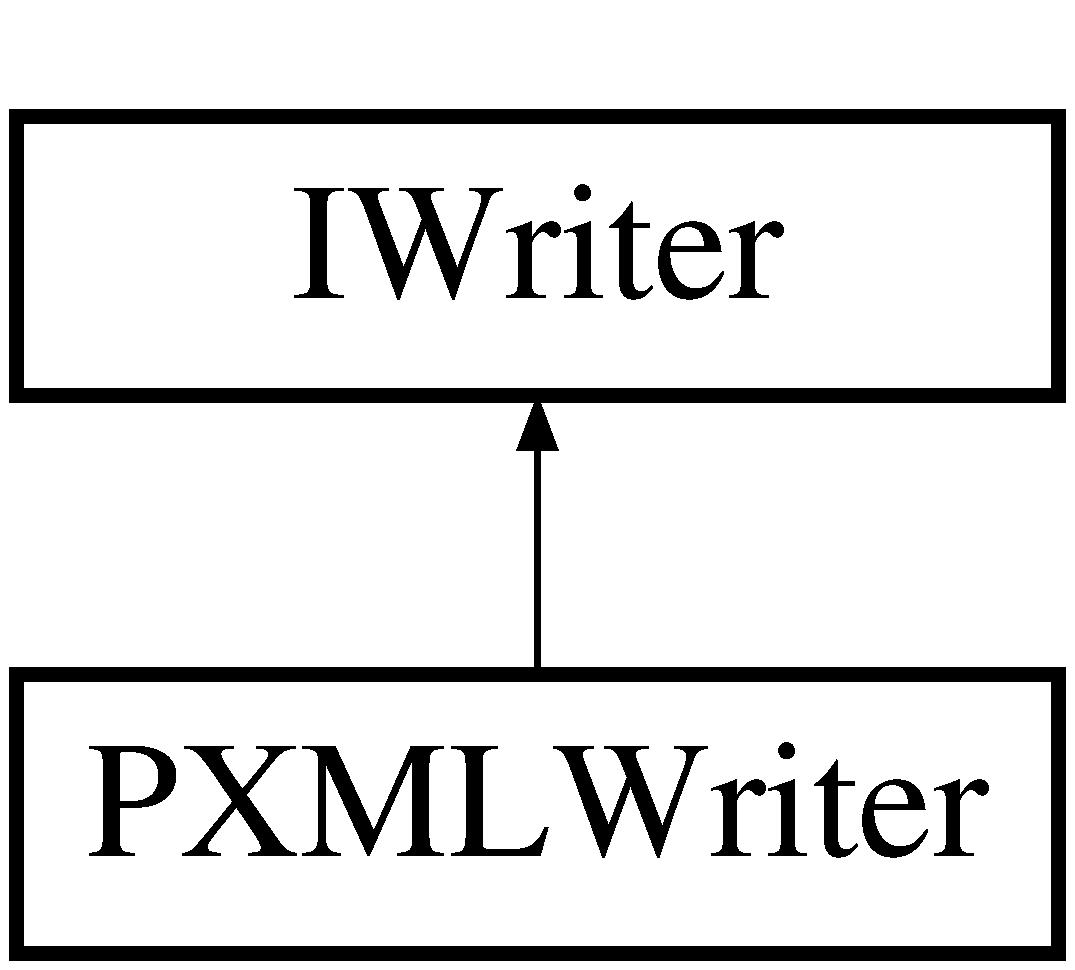
\includegraphics[height=2.000000cm]{class_p_x_m_l_writer}
\end{center}
\end{figure}
\subsection*{Public Member Functions}
\begin{DoxyCompactItemize}
\item 
{\bf \-\_\-\-\_\-construct} (\$file=\char`\"{}\char`\"{})
\item 
{\bf write} (\$message, \$level)
\end{DoxyCompactItemize}


\subsection{Constructor \& Destructor Documentation}
\index{P\-X\-M\-L\-Writer@{P\-X\-M\-L\-Writer}!\-\_\-\-\_\-construct@{\-\_\-\-\_\-construct}}
\index{\-\_\-\-\_\-construct@{\-\_\-\-\_\-construct}!PXMLWriter@{P\-X\-M\-L\-Writer}}
\subsubsection[{\-\_\-\-\_\-construct}]{\setlength{\rightskip}{0pt plus 5cm}\-\_\-\-\_\-construct (
\begin{DoxyParamCaption}
\item[{}]{\$file = {\ttfamily \char`\"{}\char`\"{}}}
\end{DoxyParamCaption}
)}\label{class_p_x_m_l_writer_a9265d0ed1be06516b2bb4a450e5ff180}
Constructeur

Constructeur du writer texten defini le fichier du log


\begin{DoxyParams}{Parameters}
{\em string} & file url du fichier de log text \\
\hline
\end{DoxyParams}


\subsection{Member Function Documentation}
\index{P\-X\-M\-L\-Writer@{P\-X\-M\-L\-Writer}!write@{write}}
\index{write@{write}!PXMLWriter@{P\-X\-M\-L\-Writer}}
\subsubsection[{write}]{\setlength{\rightskip}{0pt plus 5cm}write (
\begin{DoxyParamCaption}
\item[{}]{\$message, }
\item[{}]{\$level}
\end{DoxyParamCaption}
)}\label{class_p_x_m_l_writer_aecf647bb93e520f455d1145622b5db41}
write

Ajout d'un log implemente l'interface I\-W\-R\-I\-T\-E\-R


\begin{DoxyParams}{Parameters}
{\em string} & message log \\
\hline
\end{DoxyParams}


Implements {\bf I\-Writer} \doxyref{}{p.}{interface_i_writer_aecf647bb93e520f455d1145622b5db41}.



The documentation for this class was generated from the following file\-:\begin{DoxyCompactItemize}
\item 
D\-:/\-Documents/\-Git\-Hub/diapazen/system/\-L\-O\-G/P\-X\-M\-L\-Writer.\-class.\-php\end{DoxyCompactItemize}

\section{Request Class Reference}
\label{class_request}\index{Request@{Request}}
\subsection*{Public Member Functions}
\begin{DoxyCompactItemize}
\item 
{\bf \-\_\-\-\_\-construct} ()
\item 
{\bf get\-Controller} ()
\item 
{\bf get\-Action} ()
\item 
{\bf get\-Params} ()
\end{DoxyCompactItemize}


\subsection{Constructor \& Destructor Documentation}
\index{Request@{Request}!\-\_\-\-\_\-construct@{\-\_\-\-\_\-construct}}
\index{\-\_\-\-\_\-construct@{\-\_\-\-\_\-construct}!Request@{Request}}
\subsubsection[{\-\_\-\-\_\-construct}]{\setlength{\rightskip}{0pt plus 5cm}\-\_\-\-\_\-construct (
\begin{DoxyParamCaption}
{}
\end{DoxyParamCaption}
)}\label{class_request_a095c5d389db211932136b53f25f39685}
Constructeur 

\subsection{Member Function Documentation}
\index{Request@{Request}!get\-Action@{get\-Action}}
\index{get\-Action@{get\-Action}!Request@{Request}}
\subsubsection[{get\-Action}]{\setlength{\rightskip}{0pt plus 5cm}get\-Action (
\begin{DoxyParamCaption}
{}
\end{DoxyParamCaption}
)}\label{class_request_a189a4abe5faf11f4320d5d3f1d3d1715}
Récupère l'action

\begin{DoxyReturn}{Returns}
string Nom de l'action 
\end{DoxyReturn}
\index{Request@{Request}!get\-Controller@{get\-Controller}}
\index{get\-Controller@{get\-Controller}!Request@{Request}}
\subsubsection[{get\-Controller}]{\setlength{\rightskip}{0pt plus 5cm}get\-Controller (
\begin{DoxyParamCaption}
{}
\end{DoxyParamCaption}
)}\label{class_request_aa8b89e0bad51878addc1300cd3e95b5c}
Récupère le nom du controller

\begin{DoxyReturn}{Returns}
string Nom du controller 
\end{DoxyReturn}
\index{Request@{Request}!get\-Params@{get\-Params}}
\index{get\-Params@{get\-Params}!Request@{Request}}
\subsubsection[{get\-Params}]{\setlength{\rightskip}{0pt plus 5cm}get\-Params (
\begin{DoxyParamCaption}
{}
\end{DoxyParamCaption}
)}\label{class_request_ae32cd7c32721b02d676bb63b4b1366db}
Récupère les paramètres

\begin{DoxyReturn}{Returns}
array Nom des paramètres 
\end{DoxyReturn}


The documentation for this class was generated from the following file\-:\begin{DoxyCompactItemize}
\item 
D\-:/\-Documents/\-Git\-Hub/diapazen/system/Request.\-class.\-php\end{DoxyCompactItemize}

\section{Router Class Reference}
\label{class_router}\index{Router@{Router}}
\subsection*{Public Member Functions}
\begin{DoxyCompactItemize}
\item 
{\bf \-\_\-\-\_\-construct} ()
\end{DoxyCompactItemize}


\subsection{Constructor \& Destructor Documentation}
\index{Router@{Router}!\-\_\-\-\_\-construct@{\-\_\-\-\_\-construct}}
\index{\-\_\-\-\_\-construct@{\-\_\-\-\_\-construct}!Router@{Router}}
\subsubsection[{\-\_\-\-\_\-construct}]{\setlength{\rightskip}{0pt plus 5cm}\-\_\-\-\_\-construct (
\begin{DoxyParamCaption}
{}
\end{DoxyParamCaption}
)}\label{class_router_a095c5d389db211932136b53f25f39685}
Constructeur

Récupère le nom du controller et instancie en conséquence le controller désiré Appelle de l'action spécifié par l'url au controller Si il y a un problème on lève une exception 

The documentation for this class was generated from the following file\-:\begin{DoxyCompactItemize}
\item 
D\-:/\-Documents/\-Git\-Hub/diapazen/system/Router.\-class.\-php\end{DoxyCompactItemize}

\section{Test\-Form Class Reference}
\label{class_test_form}\index{Test\-Form@{Test\-Form}}
\subsection*{Static Public Member Functions}
\begin{DoxyCompactItemize}
\item 
static {\bf test\-Regexp} (\$regexp, \$string)
\end{DoxyCompactItemize}


\subsection{Member Function Documentation}
\index{Test\-Form@{Test\-Form}!test\-Regexp@{test\-Regexp}}
\index{test\-Regexp@{test\-Regexp}!TestForm@{Test\-Form}}
\subsubsection[{test\-Regexp}]{\setlength{\rightskip}{0pt plus 5cm}static test\-Regexp (
\begin{DoxyParamCaption}
\item[{}]{\$regexp, }
\item[{}]{\$string}
\end{DoxyParamCaption}
)\hspace{0.3cm}{\ttfamily [static]}}\label{class_test_form_aa7564e07da25006f8b901e9b2370b6d0}
Fonction qui test les une string par regexp

\begin{DoxyReturn}{Returns}
boolean 
\end{DoxyReturn}


The documentation for this class was generated from the following file\-:\begin{DoxyCompactItemize}
\item 
D\-:/\-Documents/\-Git\-Hub/diapazen/util/Test\-Form.\-class.\-php\end{DoxyCompactItemize}

\section{Text\-Writer Class Reference}
\label{class_text_writer}\index{Text\-Writer@{Text\-Writer}}
Inheritance diagram for Text\-Writer\-:\begin{figure}[H]
\begin{center}
\leavevmode
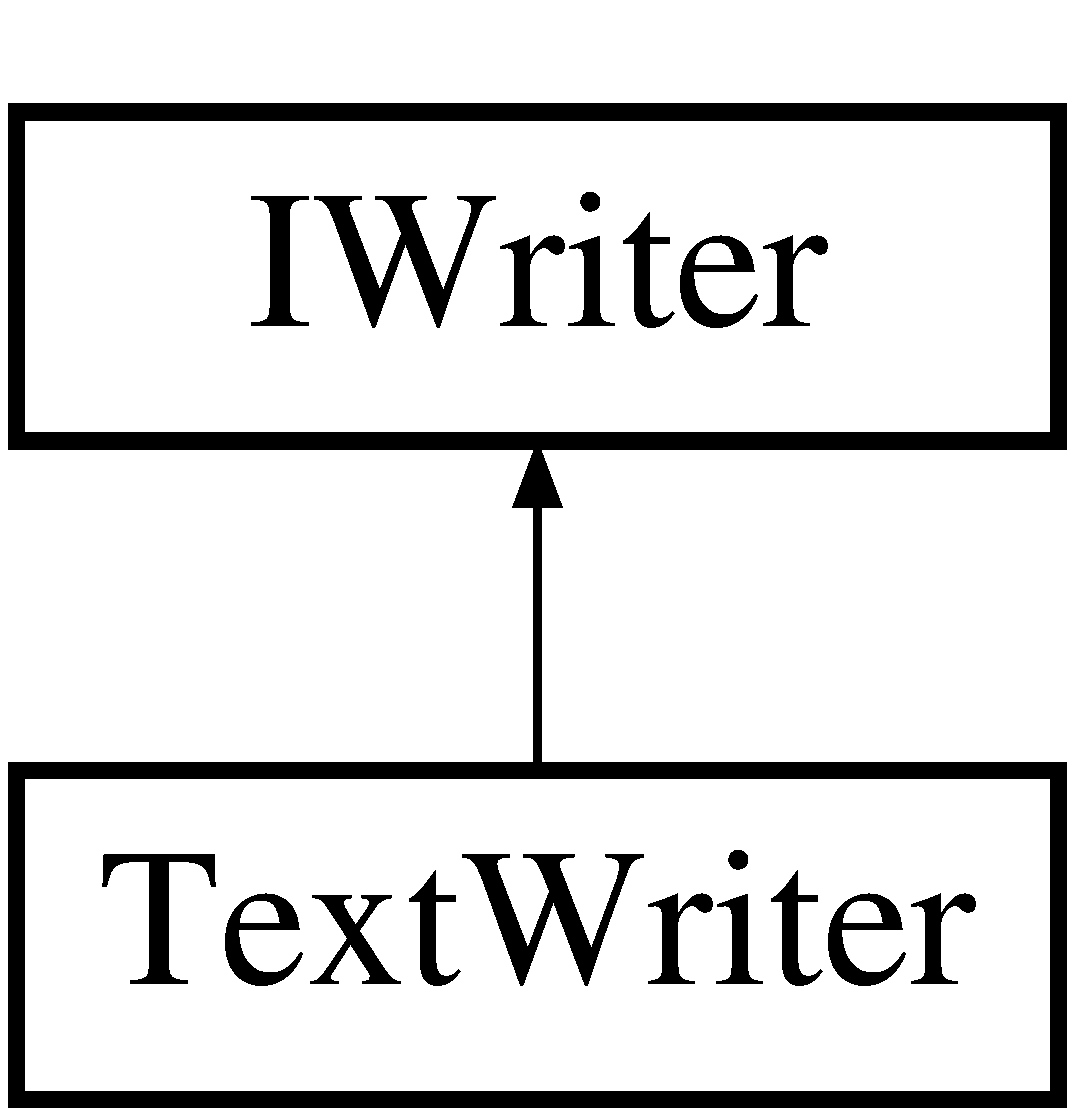
\includegraphics[height=2.000000cm]{class_text_writer}
\end{center}
\end{figure}
\subsection*{Public Member Functions}
\begin{DoxyCompactItemize}
\item 
{\bf \-\_\-\-\_\-construct} (\$file=\char`\"{}\char`\"{})
\item 
{\bf write} (\$message, \$level)
\end{DoxyCompactItemize}


\subsection{Constructor \& Destructor Documentation}
\index{Text\-Writer@{Text\-Writer}!\-\_\-\-\_\-construct@{\-\_\-\-\_\-construct}}
\index{\-\_\-\-\_\-construct@{\-\_\-\-\_\-construct}!TextWriter@{Text\-Writer}}
\subsubsection[{\-\_\-\-\_\-construct}]{\setlength{\rightskip}{0pt plus 5cm}\-\_\-\-\_\-construct (
\begin{DoxyParamCaption}
\item[{}]{\$file = {\ttfamily \char`\"{}\char`\"{}}}
\end{DoxyParamCaption}
)}\label{class_text_writer_a9265d0ed1be06516b2bb4a450e5ff180}
Constructeur

Constructeur du writer texten defini le fichier du log


\begin{DoxyParams}{Parameters}
{\em string} & file url du fichier de log text \\
\hline
\end{DoxyParams}


\subsection{Member Function Documentation}
\index{Text\-Writer@{Text\-Writer}!write@{write}}
\index{write@{write}!TextWriter@{Text\-Writer}}
\subsubsection[{write}]{\setlength{\rightskip}{0pt plus 5cm}write (
\begin{DoxyParamCaption}
\item[{}]{\$message, }
\item[{}]{\$level}
\end{DoxyParamCaption}
)}\label{class_text_writer_aecf647bb93e520f455d1145622b5db41}
write

Ajout d'un log implemente l'interface I\-W\-R\-I\-T\-E\-R


\begin{DoxyParams}{Parameters}
{\em string} & message log \\
\hline
\end{DoxyParams}


Implements {\bf I\-Writer} \doxyref{}{p.}{interface_i_writer_aecf647bb93e520f455d1145622b5db41}.



The documentation for this class was generated from the following file\-:\begin{DoxyCompactItemize}
\item 
D\-:/\-Documents/\-Git\-Hub/diapazen/system/\-L\-O\-G/Text\-Writer.\-class.\-php\end{DoxyCompactItemize}

\section{User\-Controller Class Reference}
\label{class_user_controller}\index{User\-Controller@{User\-Controller}}
Inheritance diagram for User\-Controller\-:\begin{figure}[H]
\begin{center}
\leavevmode
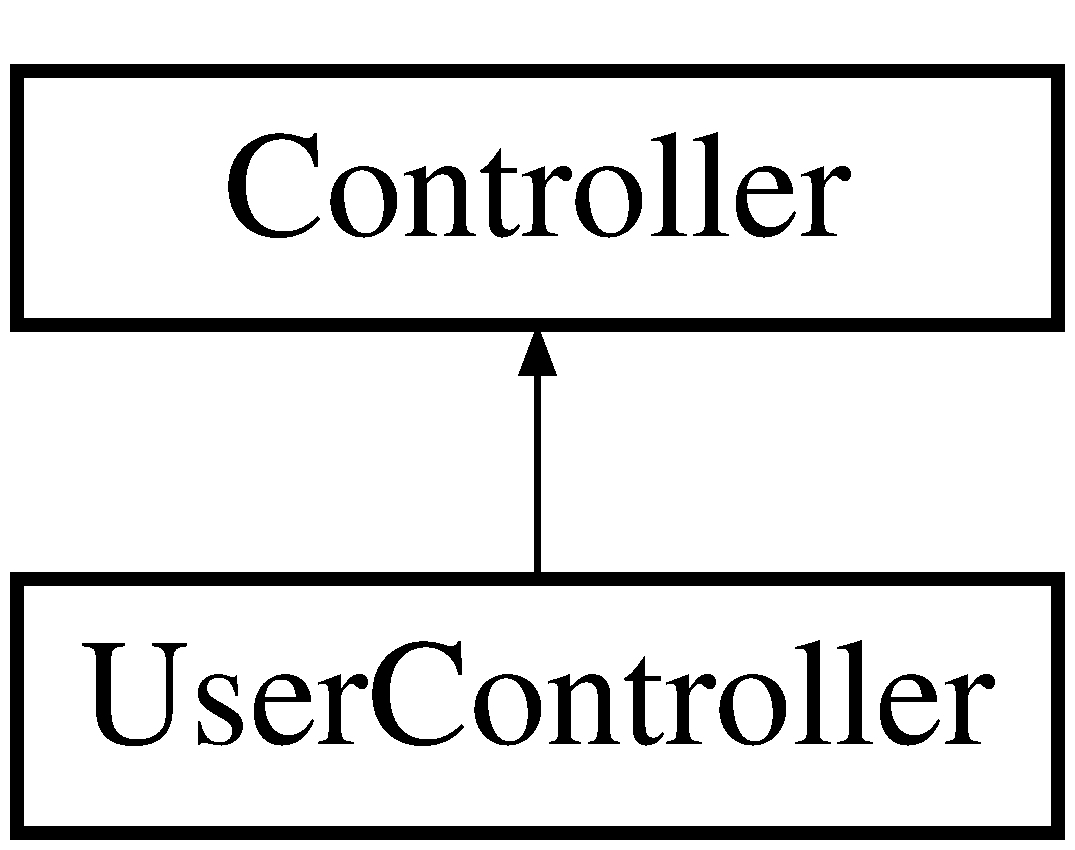
\includegraphics[height=2.000000cm]{class_user_controller}
\end{center}
\end{figure}
\subsection*{Public Member Functions}
\begin{DoxyCompactItemize}
\item 
{\bf index} (\$params=null)
\item 
{\bf login} (\$params=null)
\item 
{\bf profile} (\$params=null)
\item 
{\bf forgot} (\$params=null)
\item 
{\bf logout} (\$params=null)
\end{DoxyCompactItemize}
\subsection*{Additional Inherited Members}


\subsection{Member Function Documentation}
\index{User\-Controller@{User\-Controller}!forgot@{forgot}}
\index{forgot@{forgot}!UserController@{User\-Controller}}
\subsubsection[{forgot}]{\setlength{\rightskip}{0pt plus 5cm}forgot (
\begin{DoxyParamCaption}
\item[{}]{\$params = {\ttfamily null}}
\end{DoxyParamCaption}
)}\label{class_user_controller_a77de54d6af94e12fa48395a5f7639417}
Mot de passe oublié on verifie que l'utilisateur est d�connecter, si ce n'est pas le cas alors on redirige vers la page home. Si il est d�connecter on le dirige vers la page du mot de passe oubli�. Si l'email est pr�sent diff�rent de vide et est pr�sent dans la base de donn�es, alors on cr�er un nouveau mot de passe et on l'affecte comme nouveau mot de passe de l'utilisateur. On le lui envoi par mail et on lui notifit la pr�sence de ce mail. url\-: diapazen.\-com/user/forgot \index{User\-Controller@{User\-Controller}!index@{index}}
\index{index@{index}!UserController@{User\-Controller}}
\subsubsection[{index}]{\setlength{\rightskip}{0pt plus 5cm}index (
\begin{DoxyParamCaption}
\item[{}]{\$params = {\ttfamily null}}
\end{DoxyParamCaption}
)}\label{class_user_controller_a749de566b023589025bfebbc37537d65}
Action par défaut m�ne a la page home. url\-: diapazen.\-com/user \index{User\-Controller@{User\-Controller}!login@{login}}
\index{login@{login}!UserController@{User\-Controller}}
\subsubsection[{login}]{\setlength{\rightskip}{0pt plus 5cm}login (
\begin{DoxyParamCaption}
\item[{}]{\$params = {\ttfamily null}}
\end{DoxyParamCaption}
)}\label{class_user_controller_a9956e2e490942a4ee673a077aaf55138}
Connection à l'application On charge le mod�le de l'utilisateur, et si l'utlisateur est d�j� connecter alors on le dirige vers la page home. Sinon on v�rifie le mail et le mot de passe dans la base de donn�es et on connecte l'utilisateur et on l'envoie vers le dashboard. Si le mot de passe ou le mail est erron� alors on cr�er la variable info\-Login et on affiche le formulaire de connection. url\-: diapazen.\-com/user/login \index{User\-Controller@{User\-Controller}!logout@{logout}}
\index{logout@{logout}!UserController@{User\-Controller}}
\subsubsection[{logout}]{\setlength{\rightskip}{0pt plus 5cm}logout (
\begin{DoxyParamCaption}
\item[{}]{\$params = {\ttfamily null}}
\end{DoxyParamCaption}
)}\label{class_user_controller_a5606eef2ce2955733c1823a2e199a392}
Déconnexion de l'application Deconnect l'utilisateur et le renvoi sur la page home url\-: diapazen.\-com/user/logout \index{User\-Controller@{User\-Controller}!profile@{profile}}
\index{profile@{profile}!UserController@{User\-Controller}}
\subsubsection[{profile}]{\setlength{\rightskip}{0pt plus 5cm}profile (
\begin{DoxyParamCaption}
\item[{}]{\$params = {\ttfamily null}}
\end{DoxyParamCaption}
)}\label{class_user_controller_acc2e0b5ce375a9d6638f31a4a765f65f}
Modification des information personnelles on dirige l'utilisateur vers la page de profil, en affichant ses donn�es on v�rifie qu'il est connecter. Si tel est le cas on charge le model\-User et si l'utilisateur veut modifier ses donn�es on le fait gr�ce � ce model et on teste le mot de passe de confirmation. Si le mot de passe est erron� on ne modifie rien par contre si c'est le bon mot de passe on met alors � jour la base de donn�es, on met � jour la session et on informe l'utilisateur de la r�ussite. Si l'utilisateur veut modifier son mot de passe alors on teste le mot de passe de confirmation. Si le mot de passe est erron� on ne modifie rien par contre si c'est le bon mot de passe on met alors � jour la base de donn�es. Pour afficher les donn�es de l'utilisateur, on r�cup�re l'id de l'utilisateur, on prend les informations de la base de donn�es et on les affiche dans la vue. Si l'utilisateur est d�connecter il est dirig� vers la page home. url\-: diapazen.\-com/user/profile 

The documentation for this class was generated from the following file\-:\begin{DoxyCompactItemize}
\item 
D\-:/\-Documents/\-Git\-Hub/diapazen/app/controller/User\-Controller.\-class.\-php\end{DoxyCompactItemize}

\section{User\-Model Class Reference}
\label{class_user_model}\index{User\-Model@{User\-Model}}
Inheritance diagram for User\-Model\-:\begin{figure}[H]
\begin{center}
\leavevmode
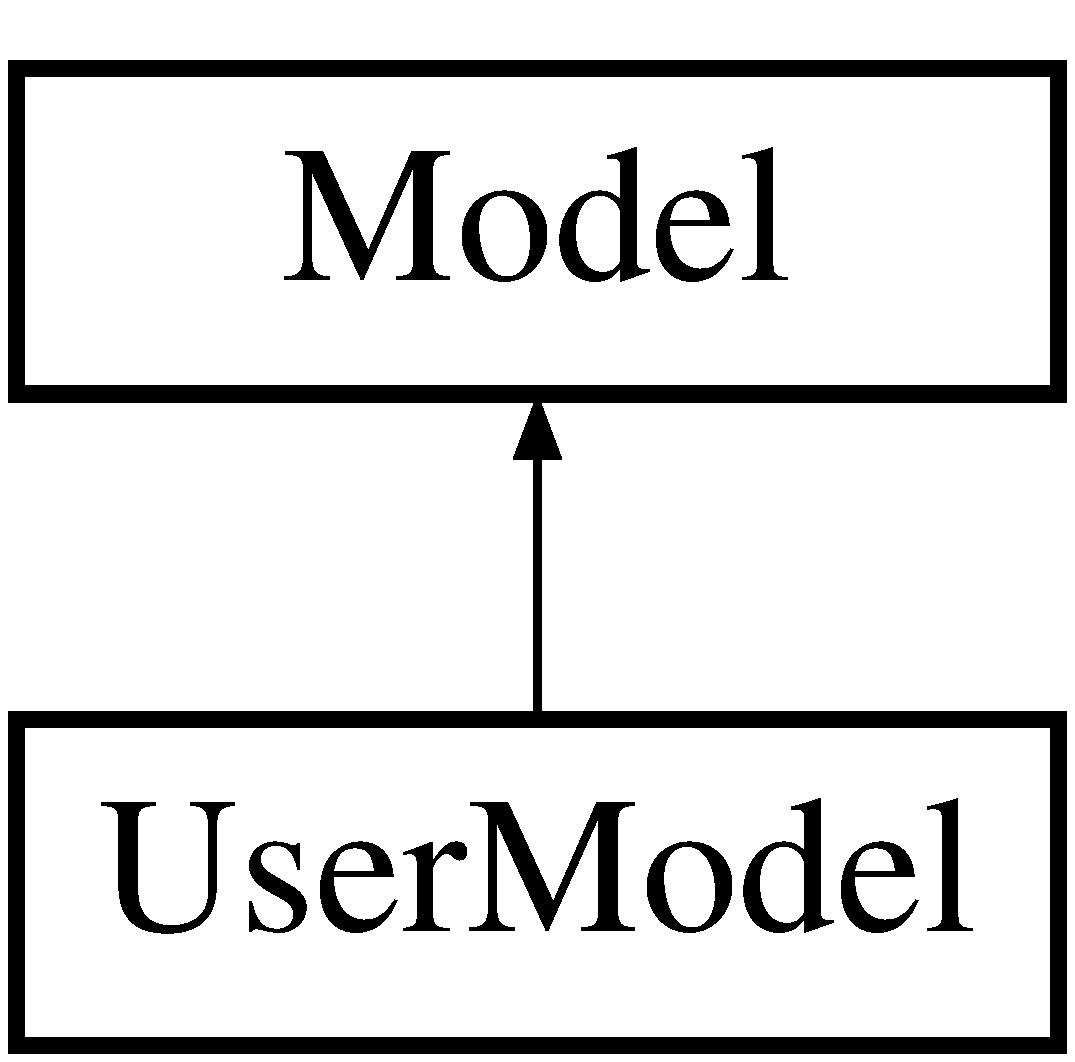
\includegraphics[height=2.000000cm]{class_user_model}
\end{center}
\end{figure}
\subsection*{Public Member Functions}
\begin{DoxyCompactItemize}
\item 
{\bf \-\_\-\-\_\-construct} ()
\item 
{\bf connection\-To\-App} (\$email, \$password, \$login\-\_\-ip=null)
\item 
{\bf update\-Connection\-Data} (\$id, \$login\-\_\-ip=null)
\item 
{\bf data\-Provider} (\$id)
\item 
{\bf registration} (\$firstname, \$lastname, \$email, \$password)
\item 
{\bf change\-User} (\$id, \$first\-Name, \$last\-Name, \$email)
\item 
{\bf change\-Password} (\$email, \$password)
\item 
{\bf check\-Password} (\$id, \$password)
\item 
{\bf generator\-Psw} (\$size=8)
\item 
{\bf is\-Email\-Registred} (\$email)
\end{DoxyCompactItemize}
\subsection*{Additional Inherited Members}


\subsection{Constructor \& Destructor Documentation}
\index{User\-Model@{User\-Model}!\-\_\-\-\_\-construct@{\-\_\-\-\_\-construct}}
\index{\-\_\-\-\_\-construct@{\-\_\-\-\_\-construct}!UserModel@{User\-Model}}
\subsubsection[{\-\_\-\-\_\-construct}]{\setlength{\rightskip}{0pt plus 5cm}\-\_\-\-\_\-construct (
\begin{DoxyParamCaption}
{}
\end{DoxyParamCaption}
)}\label{class_user_model_a095c5d389db211932136b53f25f39685}
Constructeur 

\subsection{Member Function Documentation}
\index{User\-Model@{User\-Model}!change\-Password@{change\-Password}}
\index{change\-Password@{change\-Password}!UserModel@{User\-Model}}
\subsubsection[{change\-Password}]{\setlength{\rightskip}{0pt plus 5cm}change\-Password (
\begin{DoxyParamCaption}
\item[{}]{\$email, }
\item[{}]{\$password}
\end{DoxyParamCaption}
)}\label{class_user_model_a9f4ee3e375718f0df726f3793d37e867}
Modification du mot de passe de l'utilisateur

On fait l’update du mot de passe à partir de l’email de l’utilisateur. On le hash avec Blow\-Fish (md5 et sha1 étant unsecure).


\begin{DoxyParams}[1]{Parameters}
type & {\em \$email} & email de l'utilisateur \\
\hline
type & {\em \$password} & mot de passe renseigné par l'utilisateur\\
\hline
\end{DoxyParams}
\begin{DoxyReturn}{Returns}
boolean si la modification s'est bien passé 
\end{DoxyReturn}
\index{User\-Model@{User\-Model}!change\-User@{change\-User}}
\index{change\-User@{change\-User}!UserModel@{User\-Model}}
\subsubsection[{change\-User}]{\setlength{\rightskip}{0pt plus 5cm}change\-User (
\begin{DoxyParamCaption}
\item[{}]{\$id, }
\item[{}]{\$first\-Name, }
\item[{}]{\$last\-Name, }
\item[{}]{\$email}
\end{DoxyParamCaption}
)}\label{class_user_model_a5fb6b82c3f854bf04f1c34f6e05abcf2}
Modification du profil de l'utilisateur

On fait l’update des informations à partir de l’id de l’utilisateur. Puis si l’update s’est bien passé on retourne true.


\begin{DoxyParams}[1]{Parameters}
type & {\em \$id} & id de l'utilisateur \\
\hline
 & {\em firstname} & prénom renseigné par l'utilisateur \\
\hline
 & {\em lastname} & nom de famille renseigné par l'utilisateur \\
\hline
 & {\em email} & email renseigné par l'utilisateur\\
\hline
\end{DoxyParams}
\begin{DoxyReturn}{Returns}
boolean true si la modification s'est bien passé 
\end{DoxyReturn}
\index{User\-Model@{User\-Model}!check\-Password@{check\-Password}}
\index{check\-Password@{check\-Password}!UserModel@{User\-Model}}
\subsubsection[{check\-Password}]{\setlength{\rightskip}{0pt plus 5cm}check\-Password (
\begin{DoxyParamCaption}
\item[{}]{\$id, }
\item[{}]{\$password}
\end{DoxyParamCaption}
)}\label{class_user_model_a123d0a14f688b884a7f75d918914eb52}
Vérification du mot de passe de l'utilisateur

On fait un Select pour récupérer le mot de passe de la base de donnée et on le test avec celui passé en paramètre.


\begin{DoxyParams}[1]{Parameters}
type & {\em \$id} & id de l'utilisateur \\
\hline
type & {\em \$password} & mot de passe renseigné par l'utilisateur\\
\hline
\end{DoxyParams}
\begin{DoxyReturn}{Returns}
boolean si la vérification s'est bien passé 
\end{DoxyReturn}
\index{User\-Model@{User\-Model}!connection\-To\-App@{connection\-To\-App}}
\index{connection\-To\-App@{connection\-To\-App}!UserModel@{User\-Model}}
\subsubsection[{connection\-To\-App}]{\setlength{\rightskip}{0pt plus 5cm}connection\-To\-App (
\begin{DoxyParamCaption}
\item[{}]{\$email, }
\item[{}]{\$password, }
\item[{}]{\$login\-\_\-ip = {\ttfamily null}}
\end{DoxyParamCaption}
)}\label{class_user_model_a60058296e40a7521958d12f4e6004cae}
Connexion de l'utilisateur

On test tout d’abords si l’email et le password sont bien renseignés, puis avec une requête Select on récupère les infos en faisant un Where sur le password. Puis si on a un résultat et que le password passé en paramètre correspond à celui de la base de donnée, on met à jour la dernière connection grâce à update\-Connection\-Date et on renvoie un tableau avec toutes les données.


\begin{DoxyParams}{Parameters}
{\em email} & email renseigné par l'utilisateur \\
\hline
{\em password} & mot de passe renseigné par l'utilisateur \\
\hline
{\em login\-\_\-ip} & ip de l'utilisateur\\
\hline
\end{DoxyParams}
\begin{DoxyReturn}{Returns}
array tableau avec toutes les infos si tout s’est bien passé et false sinon 
\end{DoxyReturn}
\index{User\-Model@{User\-Model}!data\-Provider@{data\-Provider}}
\index{data\-Provider@{data\-Provider}!UserModel@{User\-Model}}
\subsubsection[{data\-Provider}]{\setlength{\rightskip}{0pt plus 5cm}data\-Provider (
\begin{DoxyParamCaption}
\item[{}]{\$id}
\end{DoxyParamCaption}
)}\label{class_user_model_a905e84211fd8e818addac5810e08f045}
Récupération des données de l'utilisateur (sauf mot de passe)

On test d’abord si l’id renseigné est bon puis si c’est le cas avec une requête Select on récupère les infos en faisant un Where sur l’id. Si il y a un résultat on le renvoi sous forme de tableau.


\begin{DoxyParams}{Parameters}
{\em id} & id de l'utilisateur\\
\hline
\end{DoxyParams}
\begin{DoxyReturn}{Returns}
array un tableau avec toutes les infos si tout s’est bien passé et false sinon 
\end{DoxyReturn}
\index{User\-Model@{User\-Model}!generator\-Psw@{generator\-Psw}}
\index{generator\-Psw@{generator\-Psw}!UserModel@{User\-Model}}
\subsubsection[{generator\-Psw}]{\setlength{\rightskip}{0pt plus 5cm}generator\-Psw (
\begin{DoxyParamCaption}
\item[{}]{\$size = {\ttfamily 8}}
\end{DoxyParamCaption}
)}\label{class_user_model_a1fd2f70ce94b6cef6338d56c7cca7424}
Fonction qui génère un mot de passe aléatoire

On choisit aléatoirement un élément dans une liste de caractère autant de fois que spécifié en paramètre.


\begin{DoxyParams}[1]{Parameters}
int & {\em \$size} & taille du mot de passe(8 par defaut)\\
\hline
\end{DoxyParams}
\begin{DoxyReturn}{Returns}
retourne le mot de passe 
\end{DoxyReturn}
\index{User\-Model@{User\-Model}!is\-Email\-Registred@{is\-Email\-Registred}}
\index{is\-Email\-Registred@{is\-Email\-Registred}!UserModel@{User\-Model}}
\subsubsection[{is\-Email\-Registred}]{\setlength{\rightskip}{0pt plus 5cm}is\-Email\-Registred (
\begin{DoxyParamCaption}
\item[{}]{\$email}
\end{DoxyParamCaption}
)}\label{class_user_model_aa269ca9ad63f3b78bbdaafc35cc25d35}
Vérification si email contenu dans bdd

On fait un Select sur la table ‘dpz\-\_\-view\-\_\-users’ avec en clause Where le password passé en paramètre. Puis on test si il y a un résultat.


\begin{DoxyParams}[1]{Parameters}
type & {\em \$email} & email à vérifier \\
\hline
\end{DoxyParams}
\begin{DoxyReturn}{Returns}
boolean true si l'email est présent 
\end{DoxyReturn}
\index{User\-Model@{User\-Model}!registration@{registration}}
\index{registration@{registration}!UserModel@{User\-Model}}
\subsubsection[{registration}]{\setlength{\rightskip}{0pt plus 5cm}registration (
\begin{DoxyParamCaption}
\item[{}]{\$firstname, }
\item[{}]{\$lastname, }
\item[{}]{\$email, }
\item[{}]{\$password}
\end{DoxyParamCaption}
)}\label{class_user_model_a7da627674fce6ba1b9e7fd3ad4726124}
Enregistrement d'un nouvel utilisateur

On test d’abords si les paramètres puis si ils sont bien renseignés. Ensuite on test si l’utilisateur n’est pas déjà enregistré on fait l’insertion des données dans la table dpz\-\_\-users. On hash le mot de passe avec Blow\-Fish (md5 et sha1 étant unsecure).


\begin{DoxyParams}{Parameters}
{\em firstname} & prénom renseigné par l'utilisateur \\
\hline
{\em lastname} & nom de famille renseigné par l'utilisateur \\
\hline
{\em email} & email renseigné par l'utilisateur \\
\hline
{\em password} & mot de passe renseigné par l'utilisateur\\
\hline
\end{DoxyParams}
\begin{DoxyReturn}{Returns}
bool true si l'enregistrement s'est bien passé 
\end{DoxyReturn}
\index{User\-Model@{User\-Model}!update\-Connection\-Data@{update\-Connection\-Data}}
\index{update\-Connection\-Data@{update\-Connection\-Data}!UserModel@{User\-Model}}
\subsubsection[{update\-Connection\-Data}]{\setlength{\rightskip}{0pt plus 5cm}update\-Connection\-Data (
\begin{DoxyParamCaption}
\item[{}]{\$id, }
\item[{}]{\$login\-\_\-ip = {\ttfamily null}}
\end{DoxyParamCaption}
)}\label{class_user_model_a6df621beb2f7d7f0226657d8fa2d20a4}
Mise à jour des données de connexion de l'utilisateur (adresse ip et date de derniere connexion)

On test d’abord si l’id renseigné est bon , puis si c’est le cas on update d’abords la date de dernière connexion dans la table ‘dpz\-\_\-users’ avec une clause Where sur l’id. Puis on met à jour de la même manière l’ip.


\begin{DoxyParams}{Parameters}
{\em login\-\_\-ip} & ip de l'utilisateur\\
\hline
\end{DoxyParams}
\begin{DoxyReturn}{Returns}
bool true si la mise à jour s'est bien passé 
\end{DoxyReturn}


The documentation for this class was generated from the following file\-:\begin{DoxyCompactItemize}
\item 
D\-:/\-Documents/\-Git\-Hub/diapazen/app/model/User\-Model.\-class.\-php\end{DoxyCompactItemize}

\section{Xml\-Util Class Reference}
\label{class_xml_util}\index{Xml\-Util@{Xml\-Util}}
\subsection*{Public Member Functions}
\begin{DoxyCompactItemize}
\item 
{\bf \-\_\-\-\_\-construct} (\$file\-U\-R\-L)
\item 
{\bf add\-Node} (\$name, \$value=\char`\"{}\char`\"{}, \$attributes=null)
\item 
{\bf save\-Xml} ()
\end{DoxyCompactItemize}
\subsection*{Protected Attributes}
\begin{DoxyCompactItemize}
\item 
{\bfseries \$m\-X\-M\-L\-File} =null\label{class_xml_util_a153b0b2191fa00cd23cbf6b13a8172a1}

\item 
{\bfseries \$m\-File\-Name}\label{class_xml_util_a479215ef47678325b453fe80db5cf275}

\end{DoxyCompactItemize}


\subsection{Constructor \& Destructor Documentation}
\index{Xml\-Util@{Xml\-Util}!\-\_\-\-\_\-construct@{\-\_\-\-\_\-construct}}
\index{\-\_\-\-\_\-construct@{\-\_\-\-\_\-construct}!XmlUtil@{Xml\-Util}}
\subsubsection[{\-\_\-\-\_\-construct}]{\setlength{\rightskip}{0pt plus 5cm}\-\_\-\-\_\-construct (
\begin{DoxyParamCaption}
\item[{}]{\$file\-U\-R\-L}
\end{DoxyParamCaption}
)}\label{class_xml_util_a0dcc0033e3a77fe2eb826e2af7684d7f}
Constructeur de gestionnaire xml

Permet de recuperer un fichier xml ou le creer selon un modele pour travailler sur le fichier.


\begin{DoxyParams}{Parameters}
{\em string} & file\-U\-R\-L lien vers le fichier \\
\hline
\end{DoxyParams}


\subsection{Member Function Documentation}
\index{Xml\-Util@{Xml\-Util}!add\-Node@{add\-Node}}
\index{add\-Node@{add\-Node}!XmlUtil@{Xml\-Util}}
\subsubsection[{add\-Node}]{\setlength{\rightskip}{0pt plus 5cm}add\-Node (
\begin{DoxyParamCaption}
\item[{}]{\$name, }
\item[{}]{\$value = {\ttfamily \char`\"{}\char`\"{}}, }
\item[{}]{\$attributes = {\ttfamily null}}
\end{DoxyParamCaption}
)}\label{class_xml_util_a4218d99e8f12761e0200ac5b7af7b243}
Ajout d'un noeud dans le root


\begin{DoxyParams}{Parameters}
{\em string} & name nom du noeud \\
\hline
{\em string} & value contenu du noeud (defaut vide) \\
\hline
{\em array} & attributes tableau dattribut (key --$>$ value) \\
\hline
\end{DoxyParams}
\begin{DoxyReturn}{Returns}
simple\-X\-M\-L\-Element noed ajouté 
\end{DoxyReturn}
\index{Xml\-Util@{Xml\-Util}!save\-Xml@{save\-Xml}}
\index{save\-Xml@{save\-Xml}!XmlUtil@{Xml\-Util}}
\subsubsection[{save\-Xml}]{\setlength{\rightskip}{0pt plus 5cm}save\-Xml (
\begin{DoxyParamCaption}
{}
\end{DoxyParamCaption}
)}\label{class_xml_util_a16949d826b2a3614b30a2940013116b1}
Enregistre le xml


\begin{DoxyParams}{Parameters}
{\em string} & name nom du fichier \\
\hline
\end{DoxyParams}


The documentation for this class was generated from the following file\-:\begin{DoxyCompactItemize}
\item 
D\-:/\-Documents/\-Git\-Hub/diapazen/util/Xml\-Util.\-class.\-php\end{DoxyCompactItemize}

%--- End generated contents ---

% Index
\newpage
\phantomsection
\addcontentsline{toc}{part}{Index}
\printindex

\end{document}
